\documentclass{cmspaper}
\usepackage{graphicx}
\usepackage{amsmath}
\usepackage{amssymb}
\usepackage{subfigure}
\usepackage{multirow}
\usepackage[pdfborder=0 0 0,
            colorlinks,
            urlcolor = blue,
            linkcolor = black,
            citecolor = black,
            menucolor = black,]
           {hyperref}
%% \usepackage[colorlinks]{hyperref}
%% \usepackage{url}
\usepackage[toc,page]{appendix}
\usepackage{varioref}
\renewcommand{\appendixname}{Appendix}
%% \renewcommand{\appendixtocname}{List of appendices}

%-------------------------------------------------------------------------------
% private environments
%-------------------------------------------------------------------------------

\newcommand{\customChapter}[1]{\chapter{\boldmath #1 \unboldmath}}
\newcommand{\customSection}[1]{\section{\boldmath #1 \unboldmath}}
\newcommand{\customSubsection}[1]{\boldmath\subsection{#1}\unboldmath}
\newcommand{\customSubsubsection}[1]{\boldmath\subsubsection{#1}\unboldmath}

%-------------------------------------------------------------------------------
% technical reference definitions
%-------------------------------------------------------------------------------

\newcommand{\AppendixRef}[1]{Appendix~\ref{#1}}
\newcommand{\EquationRef}[1]{Equation~(\ref{#1})}
\newcommand{\FigureRef}[1]{Figure~\ref{#1}}
\newcommand{\ReferenceRef}[1]{Reference~\cite{#1}}
\newcommand{\SectionRef}[1]{Section~\ref{#1}}
\newcommand{\TableRef}[1]{Table~\ref{#1}}

%-------------------------------------------------------------------------------
% unit definitions
%-------------------------------------------------------------------------------

\newcommand{\fs}{\ensuremath{\mathrm{fs}}}
\newcommand{\ps}{\ensuremath{\mathrm{ps}}}
\newcommand{\ns}{\ensuremath{\mathrm{ns}}}
\newcommand{\ips}{\ensuremath{\mathrm{ps^{-1}}}}
\newcommand{\um}{\ensuremath{\mathrm{\mu m}}}
\newcommand{\mm}{\ensuremath{\mathrm{mm}}}
\newcommand{\cm}{\ensuremath{\mathrm{cm}}}
\renewcommand{\deg}{\ensuremath{^\mathrm{o}}}
\newcommand{\ifb}{\ensuremath{\mathrm{fb^{-1}}}}
\newcommand{\ipb}{\ensuremath{\mathrm{pb^{-1}}}}
\newcommand{\inb}{\ensuremath{\mathrm{nb^{-1}}}}
\newcommand{\iub}{\ensuremath{\mathrm{\mu b^{-1}}}}
\newcommand{\fb}{\ensuremath{\mathrm{fb}}}
\newcommand{\pb}{\ensuremath{\mathrm{pb}}}
\newcommand{\nb}{\ensuremath{\mathrm{nb}}}
\newcommand{\ub}{\ensuremath{\mathrm{\mu b}}}
\newcommand{\eV}{\ensuremath{\mathrm{e\kern -0.1em V}}}
\newcommand{\keV}{\ensuremath{\mathrm{ke\kern -0.1em V}}}
\newcommand{\MeV}{\ensuremath{\mathrm{Me\kern -0.1em V}}}
\newcommand{\GeV}{\ensuremath{\mathrm{Ge\kern -0.1em V}}}
\newcommand{\TeV}{\ensuremath{\mathrm{Te\kern -0.1em V}}}
\newcommand{\eVc}{\ensuremath{\mathrm{e\kern -0.1em V/}c}}
\newcommand{\keVc}{\ensuremath{\mathrm{ke\kern -0.1em V/}c}}
\newcommand{\MeVc}{\ensuremath{\mathrm{Me\kern -0.1em V/}c}}
\newcommand{\GeVc}{\ensuremath{\mathrm{Ge\kern -0.1em V/}c}}
\newcommand{\TeVc}{\ensuremath{\mathrm{Te\kern -0.1em V/}c}}
\newcommand{\eVcc}{\ensuremath{\mathrm{e\kern -0.1em V/}c^2}}
\newcommand{\keVcc}{\ensuremath{\mathrm{ke\kern -0.1em V/}c^2}}
\newcommand{\MeVcc}{\ensuremath{\mathrm{Me\kern -0.1em V/}c^2}}
\newcommand{\GeVcc}{\ensuremath{\mathrm{Ge\kern -0.1em V/}c^2}}
\newcommand{\TeVcc}{\ensuremath{\mathrm{Te\kern -0.1em V/}c^2}}
\newcommand{\Tesla}{\ensuremath{\mathrm{T}}}

\newcommand{\kB}{\ensuremath{\mathrm{kBytes}}}
\newcommand{\MB}{\ensuremath{\mathrm{MBytes}}}
\newcommand{\GB}{\ensuremath{\mathrm{GBytes}}}
\newcommand{\PB}{\ensuremath{\mathrm{PBytes}}}
\newcommand{\TB}{\ensuremath{\mathrm{TBytes}}}
\newcommand{\kBs}{\ensuremath{\mathrm{kBytes/s}}}
\newcommand{\MBs}{\ensuremath{\mathrm{MBytes/s}}}

\newcommand{\Hz}{\ensuremath{\mathrm{Hz}}}
\newcommand{\kHz}{\ensuremath{\mathrm{kHz}}}
\newcommand{\MHz}{\ensuremath{\mathrm{MHz}}}
\newcommand{\GHz}{\ensuremath{\mathrm{GHz}}}

\newcommand{\icmSQs}{\ensuremath{\mathrm{cm^{-2}s^{-1}}}}

%-------------------------------------------------------------------------------
% reconstruction variable definitions
%-------------------------------------------------------------------------------

\newcommand{\SQS}{\ensuremath{\sqrt{s}}}
\newcommand{\ILUM}{\ensuremath{{\cal L}}}
\newcommand{\TZ}{\ensuremath{t_0}}
\newcommand{\PHISIX}{\ensuremath{\mathrm{\phi_6}}}
\newcommand{\PHIZERO}{\ensuremath{\mathrm{\phi_0}}}
\newcommand{\DPHI}{\ensuremath{\mathrm{\Delta \phi}}}
\newcommand{\ETA}{\ensuremath{\mathrm{\eta}}}
\newcommand{\DZERO}{\ensuremath{\mathrm{d_0}}}
\newcommand{\DZEB}{\ensuremath{\mathrm{d_B}}}
\newcommand{\PT}{\ensuremath{p_{T}}}
\newcommand{\Y}{\ensuremath{\mathrm{y}}}
\newcommand{\BDCUTS}{\ensuremath{\mathrm{\PT(\BD)>6\,\GeV;~|\Y| < 1}}}
\newcommand{\XSBD}{\ensuremath{\mathrm{\sigma_\BD}}}
\newcommand{\XSTOT}{\ensuremath{\mathrm{\sigma_{total}}}}

\newcommand{\Br}{\ensuremath{{\cal B}}}

%-------------------------------------------------------------------------------
% CKM matrix related
%-------------------------------------------------------------------------------

\newcommand{\LAM}{\ensuremath{\mathrm{\lambda}}}
\newcommand{\RHO}{\ensuremath{\mathrm{\rho}}}
%\newcommand{\ETA}{\ensuremath{\mathrm{\eta}}}

\newcommand{\VCKM}{\ensuremath{\mathrm{V}}}
\newcommand{\VCKMd}{\ensuremath{\mathrm{V^\dagger}}}

\newcommand{\VUD}{\ensuremath{\mathrm{V_{ud}}}}
\newcommand{\VUS}{\ensuremath{\mathrm{V_{us}}}}
\newcommand{\VUB}{\ensuremath{\mathrm{V_{ub}}}}
\newcommand{\VCD}{\ensuremath{\mathrm{V_{cd}}}}
\newcommand{\VCB}{\ensuremath{\mathrm{V_{cb}}}}
\newcommand{\VCS}{\ensuremath{\mathrm{V_{cs}}}}
\newcommand{\VTB}{\ensuremath{\mathrm{V_{tb}}}}
\newcommand{\VTD}{\ensuremath{\mathrm{V_{td}}}}
\newcommand{\VTS}{\ensuremath{\mathrm{V_{ts}}}}

\newcommand{\VUDs}{\ensuremath{\mathrm{V^*_{ud}}}}
\newcommand{\VUBs}{\ensuremath{\mathrm{V^*_{ub}}}}
\newcommand{\VCDs}{\ensuremath{\mathrm{V^*_{cd}}}}
\newcommand{\VCBs}{\ensuremath{\mathrm{V^*_{cb}}}}
\newcommand{\VCSs}{\ensuremath{\mathrm{V^*_{cs}}}}
\newcommand{\VTBs}{\ensuremath{\mathrm{V^*_{tb}}}}
\newcommand{\VTDs}{\ensuremath{\mathrm{V^*_{td}}}}
\newcommand{\VTSs}{\ensuremath{\mathrm{V^*_{ts}}}}

%-------------------------------------------------------------------------------
% physics parameter definitions
%-------------------------------------------------------------------------------

\newcommand{\EPS}{\ensuremath{\varepsilon}}
\newcommand{\DIL}{\ensuremath{\rm D}}
\newcommand{\EPSDSQ}{\ensuremath{\rm \varepsilon D^2}}

\newcommand{\SINTA}{\ensuremath{\sin 2 \alpha}}
\newcommand{\SINTB}{\ensuremath{\sin 2 \beta}}

\newcommand{\PHIDNP}{\ensuremath{\mathrm{\phi^d_{NP}}}}
\newcommand{\PHISNP}{\ensuremath{\mathrm{\phi^s_{NP}}}}

\newcommand{\FU}{\ensuremath{\mathrm{f_u}}}
\newcommand{\FD}{\ensuremath{\mathrm{f_d}}}
\newcommand{\FS}{\ensuremath{\mathrm{f_s}}}
\newcommand{\FLB}{\ensuremath{\mathrm{f_{\Lambda_B}}}}
\newcommand{\EPSB}{\ensuremath{\varepsilon_\mathrm{b}}}

\newcommand{\GBS}{\ensuremath{\Gamma_s}}
\newcommand{\DGBS}{\ensuremath{\Delta \Gamma_s}}
\newcommand{\MBS}{\ensuremath{m_\BS}}
\newcommand{\DMS}{\ensuremath{\Delta m_s}}
\newcommand{\XS}{\ensuremath{x_s}}

\newcommand{\GBD}{\ensuremath{\Gamma_\mathrm{d}}}
\newcommand{\DGBD}{\ensuremath{\Delta \Gamma_\mathrm{d}}}
\newcommand{\DG}{\ensuremath{\Delta\Gamma}}
\newcommand{\DGG}{\ensuremath{\Delta\Gamma/\Gamma}}
\newcommand{\DGGS}{\ensuremath{\Delta\Gamma_s/\Gamma_s}}
\newcommand{\MBD}{\ensuremath{m_d}}
\newcommand{\DMD}{\ensuremath{\Delta m_d}}
\newcommand{\XD}{\ensuremath{x_d}}

\newcommand{\MT}{\ensuremath{m_t}}

%-------------------------------------------------------------------------------
% particle definitions
%-------------------------------------------------------------------------------

% single particles - bosons
\newcommand{\GAM}{\ensuremath{\gamma}}
\newcommand{\Z}{\ensuremath{Z}}
\newcommand{\W}{\ensuremath{W}}
\newcommand{\WP}{\ensuremath{W^+}}
\newcommand{\WM}{\ensuremath{W^-}}
\newcommand{\WPM}{\ensuremath{W^\pm}}
\newcommand{\WMP}{\ensuremath{W^\mp}}
\newcommand{\Higgs}{\ensuremath{H}}

% single particles - leptons
\newcommand{\EL}{\ensuremath{e}}
\newcommand{\ELP}{\ensuremath{e^+}}
\newcommand{\ELM}{\ensuremath{e^-}}
\newcommand{\MU}{\ensuremath{\mu}}
\newcommand{\MUP}{\ensuremath{\mu^+}}
\newcommand{\MUM}{\ensuremath{\mu^-}}
\newcommand{\TAU}{\ensuremath{\tau}}
\newcommand{\TAUP}{\ensuremath{\tau^+}}
\newcommand{\TAUM}{\ensuremath{\tau^-}}
\newcommand{\LP}{\ensuremath{\ell^{+}}}
\newcommand{\LM}{\ensuremath{\ell^{-}}}
\newcommand{\NL}{\ensuremath{\nu_{\ell}}}
\newcommand{\NLB}{\ensuremath{\overline{\nu}_{\ell}}}

% single particles - quarks
\newcommand{\up}{\ensuremath{u}}
\newcommand{\down}{\ensuremath{d}}
\newcommand{\strange}{\ensuremath{s}}
\newcommand{\charm}{\ensuremath{c}}
\newcommand{\bottom}{\ensuremath{b}}
\newcommand{\topquark}{\ensuremath{t}}
\newcommand{\ubar}{\ensuremath{\bar{u}}}
\newcommand{\dbar}{\ensuremath{\bar{d}}}
\newcommand{\sbar}{\ensuremath{\bar{s}}}
\newcommand{\cbar}{\ensuremath{\bar{c}}}
\newcommand{\bbar}{\ensuremath{\bar{b}}}
\newcommand{\tbar}{\ensuremath{\bar{t}}}




% single particles - B hadrons
\newcommand{\B}{\ensuremath{B}}
\newcommand{\BU}{\ensuremath{\mathrm{B_u}}}
\newcommand{\BUP}{\ensuremath{\mathrm{B^+}}}
\newcommand{\BUM}{\ensuremath{\mathrm{B^-}}}
\newcommand{\BD}{\ensuremath{\mathrm{B^0}}}
\newcommand{\BDB}{\ensuremath{\mathrm{\overline{B^0}}}}
\newcommand{\BS}{\ensuremath{\mathrm{B_s}}}
\newcommand{\BSB}{\ensuremath{\mathrm{\overline{B}_s}}}
\newcommand{\BC}{\ensuremath{\mathrm{B_c}}}
\newcommand{\BCP}{\ensuremath{\mathrm{B_c^+}}}
\newcommand{\BCM}{\ensuremath{\mathrm{B_c^-}}}
\newcommand{\LB}{\ensuremath{\mathrm{\Lambda_b}}}
\newcommand{\LBB}{\ensuremath{\mathrm{\overline{\Lambda}_b}}}

% single particles - charmed hadrons
\newcommand{\D}{\ensuremath{D}}
\newcommand{\DZ}{\ensuremath{\mathrm{D^0}}}
\newcommand{\DZB}{\ensuremath{\mathrm{\overline{D}^0}}}
\newcommand{\DP}{\ensuremath{\mathrm{D^+}}}
\newcommand{\DM}{\ensuremath{\mathrm{D^-}}}
\newcommand{\DS}{\ensuremath{\mathrm{D_s}}}
\newcommand{\DSP}{\ensuremath{\mathrm{D^+_s}}}
\newcommand{\DSM}{\ensuremath{\mathrm{D^-_s}}}
\newcommand{\DSPM}{\ensuremath{\mathrm{D^\pm_s}}}
\newcommand{\DSMP}{\ensuremath{\mathrm{D^\mp_s}}}
\newcommand{\DSS}{\ensuremath{\mathrm{D^*_s}}}
\newcommand{\DSSP}{\ensuremath{\mathrm{D^{*\,+}_s}}}
\newcommand{\DSSM}{\ensuremath{\mathrm{D^{*\,-}_s}}}
\newcommand{\DSSPM}{\ensuremath{\mathrm{D^{*\,\pm}_s}}}
\newcommand{\DSSMP}{\ensuremath{\mathrm{D^{*\,\mp}_s}}}
\newcommand{\LC}{\ensuremath{\mathrm{\Lambda_c}}}
\newcommand{\LCP}{\ensuremath{\mathrm{\Lambda_c^+}}}
\newcommand{\LCM}{\ensuremath{\mathrm{\Lambda_c^-}}}
\newcommand{\SCZ}{\ensuremath{\mathrm{\Sigma_c^0}}}
\newcommand{\SCP}{\ensuremath{\mathrm{\Sigma_c^+}}}
\newcommand{\SCPP}{\ensuremath{\mathrm{\Sigma_c^{++}}}}

% single particles - quarkonia
\newcommand{\UPSI}{\ensuremath{\Upsilon}}
\newcommand{\JPSI}{\ensuremath{\mathrm{J/\psi}}}
\newcommand{\PHI}{\ensuremath{\phi}}

% single particles - kaons
\newcommand{\K}{\ensuremath{K}}
\newcommand{\KP}{\ensuremath{\mathrm{K^+}}}
\newcommand{\KM}{\ensuremath{\mathrm{K^-}}}
\newcommand{\KPM}{\ensuremath{\mathrm{K^\pm}}}
\newcommand{\KMP}{\ensuremath{\mathrm{K^\mp}}}
\newcommand{\KZ}{\ensuremath{\mathrm{K^0}}}
\newcommand{\KZB}{\ensuremath{\mathrm{\overline{K}^0}}}
\newcommand{\KS}{\ensuremath{\mathrm{K^*}}}
\newcommand{\KSZ}{\ensuremath{\mathrm{K^{*\,0}}}}
\newcommand{\KZS}{\ensuremath{\mathrm{K^0_S}}}
\newcommand{\KZL}{\ensuremath{\mathrm{K^0_L}}}
\newcommand{\LS}{\ensuremath{\mathrm{\Lambda}}}
\newcommand{\SSZ}{\ensuremath{\mathrm{\Sigma^0}}}
\newcommand{\SSP}{\ensuremath{\mathrm{\Sigma^{+}}}}
\newcommand{\SSM}{\ensuremath{\mathrm{\Sigma^{-}}}}

% single particles - pions
\newcommand{\PI}{\ensuremath{\pi}}
\newcommand{\PIZ}{\ensuremath{\pi^0}}
\newcommand{\PIP}{\ensuremath{\pi^+}}
\newcommand{\PIM}{\ensuremath{\pi^-}}

% single particles - protons
\newcommand{\PR}{\ensuremath{p}}
\newcommand{\PRB}{\ensuremath{\overline{p}}}

% particle pairs
\newcommand{\EE}{\ensuremath{e^+e^-}}
\newcommand{\PPBAR}{\ensuremath{p\overline{p}}}
\newcommand{\BBBAR}{\ensuremath{b\overline{b}}}
\newcommand{\CCBAR}{\ensuremath{c\overline{c}}}
\newcommand{\ZZ}{\ensuremath{ZZ}}
\newcommand{\WW}   {\ensuremath{\WP\WM}}
\newcommand{\TTBAR}{\ensuremath{t \bar{t}}}

% more complicated particle combination
\newcommand{\WPlusJets}{\ensuremath{W\mathrm{+Jets}}}
\newcommand{\WPlusGamma}{\ensuremath{W\mathrm{+}\gamma}}
\newcommand{\Wb}{\ensuremath{Wb}}
\newcommand{\Wc}{\ensuremath{Wc}}
\newcommand{\Wbb}{\ensuremath{Wbb}}
\newcommand{\Wcc}{\ensuremath{Wcc}}

%-------------------------------------------------------------------------------
% particle decay chain definitions
%-------------------------------------------------------------------------------

% helper
\renewcommand{\to}{\ensuremath{\rightarrow}}

% Higgs decays
\newcommand{\HiggsToWW}   {\ensuremath{\Higgs \to \WP\WM}}
\newcommand{\HiggsToZZ}   {\ensuremath{\Higgs \to \ZZ}}
\newcommand{\HiggsToZZToFourL} {\ensuremath{\Higgs \to \ZZ \to \LP\LM\LP\LM}}
\newcommand{\ZToTauTau}   {\ensuremath{\Z \to \TAUP\TAUM}}
\newcommand{\ZToEE}       {\ensuremath{\Z \to \Ep\Em}}
\newcommand{\ZToMuMu}     {\ensuremath{\Z \to \Mup\Mum}}
\newcommand{\ZToEEGamma}       {\ensuremath{\Z \to \Ep\Em\gamma}}
\newcommand{\ZToLL}       {\ensuremath{\Z \to \LP\LM}}
\newcommand{\HiggsToGammaGamma} {\ensuremath{\Higgs \to \gamma\gamma}}


% Lambda_b hadronic decays
\newcommand{\LBPRDZPI}   {\ensuremath{\LB \to \PR \DZ \PIP}}
\newcommand{\LBLCDS}     {\ensuremath{\LB \to \LCP \DSM}}
\newcommand{\LBLCDSS}    {\ensuremath{\LB \to \LCP \DSSM}}
\newcommand{\LBLCDSPIPI} {\ensuremath{\LB \to \LCP \DSM \PIP \PIM}}
\newcommand{\LBLCDSSPIPI}{\ensuremath{\LB \to \LCP \DSSM \PIP \PIM}}
\newcommand{\LBPRDS}     {\ensuremath{\LB \to \PR \DSM}}
\newcommand{\LBPRDSS}    {\ensuremath{\LB \to \PR \DSSM}}
\newcommand{\LBPRDSPIPI} {\ensuremath{\LB \to \PR \DSM \PIP \PIM}}
\newcommand{\LBPRDSSPIPI}{\ensuremath{\LB \to \PR \DSSM \PIP \PIM}}
\newcommand{\LBLCPI}     {\ensuremath{\LB \to \LCP \PIM}}
\newcommand{\LBLCPIPIPI} {\ensuremath{\LB \to \LCP \PIM \PIP \PIM}}
\newcommand{\LBSCZPIPI}  {\ensuremath{\LB \to \SCZ \PIM \PIP}}
\newcommand{\LBSCPPPIPI} {\ensuremath{\LB \to \SCPP \PIM \PIM}}
\newcommand{\LBPRPI}     {\ensuremath{\LB \to \PR \PIM}}
\newcommand{\LBPRPIPIPI} {\ensuremath{\LB \to \PR \PIM \PIP \PIM}}
\newcommand{\LBPRK}      {\ensuremath{\LB \to \PR \KM}}

% Lambda_c hadronic decays
\newcommand{\LCPRKPI}   {\ensuremath{\LCP \to \PR \KM \PIP}}
\newcommand{\LCLSPIPIPI}{\ensuremath{\LCP \to \LS \PIP \PIM \PIP}}
\newcommand{\LCLSPI}    {\ensuremath{\LCP \to \LS \PIP}}

% Sigma_c hadronic decays
\newcommand{\SCZLCPI}   {\ensuremath{\SCZ \to \LCP \PIM}}
\newcommand{\SCPPLCPI}  {\ensuremath{\SCPP \to \LCP \PIP}}

% Bs hadronic decays
\newcommand{\BSDSPI}   {\ensuremath{\BS \to \DSM \PIP}}
\newcommand{\BSDSSPI}  {\ensuremath{\BS \to \DSSM \PIP}}
\newcommand{\BSDSTPI}  {\ensuremath{\BS \to \DSM \PIP \PIP \PIM}}
\newcommand{\BSDSSTPI} {\ensuremath{\BS \to \DSSM \PIP \PIP \PIM}}
\newcommand{\BSDSDS}   {\ensuremath{\BS \to \DSM \DSP}}
\newcommand{\BSDSSDS}  {\ensuremath{\BS \to \DSSPM \DSMP}}
\newcommand{\BSDSSDSS} {\ensuremath{\BS \to \DSSM \DSSP}}
\newcommand{\BSDSKPHI} {\ensuremath{\BS \to \DSPM \KMP \PHI }}
\newcommand{\BSDSSKPHI}{\ensuremath{\BS \to \DSSPM \KMP \PHI }}
\newcommand{\BSKK}     {\ensuremath{\BS \to \KM \KP}}
\newcommand{\BSKPI}    {\ensuremath{\BS \to \KM \PIP}}

% Bs leptonic decays
\newcommand{\BSJPSIPHI}{\ensuremath{\BS \to \JPSI \PHI}}
\newcommand{\BSNLDSX}  {\ensuremath{\BS \to \NL \LP \DSM X}}

% Bd hadronic decays
\newcommand{\BDPIPI}   {\ensuremath{\BD \to \PIM \PIP}}
\newcommand{\BDPIK}    {\ensuremath{\BD \to \PIM \KP}}
\newcommand{\BDJPSIKS} {\ensuremath{\BD \to \JPSI \KZS}}

% Ds* decays
\newcommand{\DSSDSGP}  {\ensuremath{\DSS \to \DS \gamma,\PIZ}}

% Ds decays
\newcommand{\DSPHIPI}  {\ensuremath{\DSM \to \PHI \PIM}}
\newcommand{\DSKSK}    {\ensuremath{\DSM \to \KSZ \KM}}
\newcommand{\DSPIPIPI} {\ensuremath{\DSM \to \PIM \PIP \PIM}}
\newcommand{\DSKZSK}   {\ensuremath{\DSM \to \KZS \KM}}
\newcommand{\DSTPI}    {\ensuremath{\DSM \to \PIM \PIM \PIP}}
\newcommand{\DSKKZSPIPI}{\ensuremath{\DSM \to \KP \KZS \PIM \PIM}}
\newcommand{\DSPHITPI} {\ensuremath{\DSM \to \PHI \PIM \PIM \PIP}}
\newcommand{\DSKPIPI}  {\ensuremath{\DSM \to \KM \PIM \PIP}}
\newcommand{\DSNLLPHIX}{\ensuremath{\DSM \to \NLB \LP \PHI   X}}
\newcommand{\DSALL}    {\ensuremath{\DSM \to \rm all \,\, above }}

% D decays
\newcommand{\DZKPI}    {\ensuremath{\DZ \to \KM \PIP}}
\newcommand{\DZKPIPIPI}{\ensuremath{\DZ \to \KM \PIP \PIM \PIP}}

% Lambda_c hadronic decays
\newcommand{\LSPRPI}   {\ensuremath{\LS \to \PR \PIM}}

% Phi decays
\newcommand{\PHIKK}    {\ensuremath{\PHI \to \KM \KP}}

% K* decays
\newcommand{\KSKPI}    {\ensuremath{\KSZ \to \KP \PIM}}

% Kshort decays
\newcommand{\KZSPIPI}  {\ensuremath{\KZS \to \KP \PIM}}


\newcommand{\CLs}{\ensuremath{CL_\mathrm{s}}}
\newcommand{\CLb}{\ensuremath{CL_\mathrm{b}}}
\newcommand{\CLsb}{\ensuremath{CL_\mathrm{s+b}}}

\newcommand{\grad}{\ensuremath{^{\circ}}}
%
% Special user made math symbols
%
\newcommand{\lsim}{\raisebox{-1.5mm}{$\:\stackrel{\textstyle{<}}{\textstyle{\sim}}\:$}}
\newcommand{\gsim}{\raisebox{-1.5mm}{$\:\stackrel{\textstyle{>}}{\textstyle{\sim}}\:$}}

% particles

\newcommand{\pipm}{\ensuremath{\pi^{\pm}}}
\newcommand{\pizero}{\ensuremath{\pi^{0}}}
\newcommand{\Kpm}{\ensuremath{K^{\pm}}}
\newcommand{\Hi}{\ensuremath{H}}
\newcommand{\Wjets}{\ensuremath{W+\mathrm{jets}}}
\newcommand{\Zjets}{\ensuremath{Z+\mathrm{jets}}}
\newcommand{\Wt}{\ensuremath{\mathrm{Wt}}}
\newcommand{\Wstar}{\ensuremath{W^{*}}}
\newcommand{\Wparenthesisstar}{\ensuremath{W^{(*)}}}
\newcommand{\Zstar}{\ensuremath{Z^{*}}}
\newcommand{\WZ}{\ensuremath{\W\Z}}
\newcommand{\E}{\ensuremath{\mathrm{e}}}
\newcommand{\Ep}{\ensuremath{\mathrm{e}^{+}}}
\newcommand{\Em}{\ensuremath{\mathrm{e}^{-}}}
\newcommand{\Epm}{\ensuremath{\mathrm{e}^{\pm}}}
\newcommand{\Emp}{\ensuremath{\mathrm{e}^{\mp}}}
\newcommand{\Mu}{\ensuremath{\mu}}
\newcommand{\Mup}{\ensuremath{\mu^{+}}}
\newcommand{\Mum}{\ensuremath{\mu^{-}}}
\newcommand{\Mupm}{\ensuremath{\mu^{\pm}}}
\newcommand{\Mump}{\ensuremath{\mu^{\mp}}}
\newcommand{\Tau}{\ensuremath{\tau}}
\newcommand{\Taup}{\ensuremath{\tau^{+}}}
\newcommand{\Taum}{\ensuremath{\tau^{-}}}
\newcommand{\Taupm}{\ensuremath{\tau^{\pm}}}
\newcommand{\Taump}{\ensuremath{\tau^{\mp}}}
\newcommand{\Nu}{\ensuremath{\nu}}
\newcommand{\Nubar}{\ensuremath{\bar{\nu}}}
\newcommand{\Lep}{\ensuremath{\ell}}
\newcommand{\Lepp}{\ensuremath{\ell^{+}}}
\newcommand{\Lepm}{\ensuremath{\ell^{-}}}
\newcommand{\Lprime}{\ensuremath{\Lep^{\prime}}}
\newcommand{\Prot}{\ensuremath{p}}
\newcommand{\Pbar}{\ensuremath{\bar{p}}}
\newcommand{\PP}{\Prot\Prot}
\newcommand{\PPbar}{\Prot\Pbar}
\newcommand{\ttbar}{\ensuremath{t\bar{t}}}
\newcommand{\qq}{\ensuremath{\mathrm{q}\mathrm{q}}}
\newcommand{\bbbar}{\ensuremath{\mathrm{b}\bar{\mathrm{b}}}}
\newcommand{\Wtb}{\ensuremath{\W\mathrm{t}\mathrm{b}}}
\newcommand{\Top}{\ensuremath{\mathrm{t}}}
\newcommand{\Bot}{\ensuremath{\mathrm{b}}}
\newcommand{\Atop}{\ensuremath{\bar{\mathrm{t}}}}
\newcommand{\Abot}{\ensuremath{\bar{\mathrm{b}}}}
% arrow
\newcommand{\To}{\ensuremath{\rightarrow}}

% masses
\newcommand{\mHi}{\ensuremath{m_{\mathrm{Higgs}}}}
\newcommand{\mW}{\ensuremath{m_{\mathrm{W}}}}
\newcommand{\mZ}{\ensuremath{m_{\mathrm{Z}}}}
\newcommand{\mll}{\ensuremath{m_{\Lep\Lep}}}


% kinematics
\newcommand{\pt}{\ensuremath{p_\mathrm{T}}}
\newcommand{\ptHat}{\ensuremath{\hat{p_\mathrm{T}}}}
\newcommand{\ptveto}{\ensuremath{\pt^\mathrm{veto}}}
\newcommand{\ptl}{\ensuremath{p_\perp^{\Lep}}}
\newcommand{\ptlmax}{\ensuremath{p_{\mathrm{T}}^{\Lep,\mathrm{max}}}}
\newcommand{\ptlmin}{\ensuremath{p_{\mathrm{T}}^{\Lep,\mathrm{min}}}}
\newcommand{\met}{\ensuremath{\Et^{\mathrm{miss}}}}
\newcommand{\delphill}{\ensuremath{\Delta\phi_{\Lep\Lep}}}
\newcommand{\deletall}{\ensuremath{\Delta\eta_{\Lep\Lep}}}
\newcommand{\delphimetl}{\ensuremath{\Delta\phi_{\met\Lep}}}
\newcommand{\deltaRll}{\ensuremath{\Delta\mathrm{R}_{\Lep\Lep}}}
\newcommand{\delphimetdilep}{\ensuremath{\Delta\phi_{\met,\Lep\Lep}}}
\newcommand{\delphimetLeadingJet}{\ensuremath{\Delta\phi_{\met,\mathrm{leading\ jet}}}}
\newcommand{\Et}{\ensuremath{E_\mathrm{T}}}
\newcommand{\delR}{\ensuremath{\Delta R}}
\newcommand{\Eta}{\ensuremath{\eta}}
\newcommand{\mT}{\ensuremath{m_{T}^{\ell\ell \met}}}


%efficiencies
\newcommand{\effsig}{\ensuremath{\varepsilon_{\mathrm{bkg}}^{\mathrm{S}}}}
\newcommand{\effnorm}{\ensuremath{\varepsilon_{\mathrm{bkg}}^{\mathrm{N}}}}
\newcommand{\Nsig}{\ensuremath{N_{\mathrm{bkg}}^{\mathrm{S}}}}
\newcommand{\Nnorm}{\ensuremath{N_{\mathrm{bkg}}^{\mathrm{N}}}}
\newcommand{\epsilonFake}{\ensuremath{\varepsilon_{\mathrm{fake}}}}

% processes
\newcommand{\dyee}{\ensuremath{Z/\gamma^*\to ee}}
\newcommand{\dymm}{\ensuremath{Z/\gamma^*\to\mu\mu}}
\newcommand{\dytt}{\ensuremath{Z/\gamma^*\to\tau\tau}}
\newcommand{\dyll}{\ensuremath{Z/\gamma^*\to\ell\ell}}
\newcommand{\dy}{\ensuremath{Z/\gamma^*}}
\newcommand{\zee}{\ensuremath{Z\to ee}}
\newcommand{\zmm}{\ensuremath{Z\to\mu\mu}}
\newcommand{\ztt}{\ensuremath{Z\to\tau\tau}}
%\newcommand{\ttbar}{\ensuremath{t\bar{t}}}
\newcommand{\ppww}{\ensuremath{pp \to W^+W^-}}
\newcommand{\wwll}{\ensuremath{WW\to \ell^+\ell^-}}
\newcommand{\wwlnln}{\ensuremath{W^+W^-\to \ell^+\nu \ell^-\bar{\nu}}}
\newcommand{\ww}{\ensuremath{WW}}
\newcommand{\wwpm}{\ensuremath{W^+W^-}}
\newcommand{\hww}{\ensuremath{H\to W^+W^-}}
\newcommand{\wz}{\ensuremath{WZ}}
\newcommand{\zz}{\ensuremath{ZZ}}
\newcommand{\wgamma}{\ensuremath{W\gamma}}
\newcommand{\wjets}{\ensuremath{W+}jets} 
\newcommand{\tw}{\ensuremath{tW}} 
\newcommand{\singletopt}{\ensuremath{t} ($t$-chan)} 
\newcommand{\singletops}{\ensuremath{t} ($s$-chan)} 
\newcommand{\z}{\ensuremath{\mathrm{Z}}}
\newcommand{\routin}{\ensuremath{R_{out/in}}}

%other 
\def\fixme{({\bf FixMe})}
\newcommand{\ee}{\ensuremath{ee}}
\newcommand{\emu}{\ensuremath{e\mu}}
\def\mm{\ensuremath{\mu\mu}}

% integrated luminosity
\newcommand{\intlumi}{4.9~\ifb}


\setcounter{topnumber}{1}
\setcounter{bottomnumber}{1}
\setcounter{secnumdepth}{6}
%===================================================================================================
\begin{document}
\begin{titlepage}

  \analysisnote{2012/XXX}

  \date{\today}

  \title{Electron Efficiency Measurement Using the Radiative \ZToEEGamma\ Sample}

  \begin{Authlist}
%
Da An, Si Xie.
\Instfoot{caltech}{California Institute of Technology, Pasadena, USA}
Valere Lambert.
\Instfoot{cern}{CERN, Switzerland}
Allison Christian, Markus Klute.
\Instfoot{ucsd}{Massachusetts Institute of Technology, Cambridge, USA}
%

\end{Authlist}


  \begin{abstract}
  In this note, we report a new method for measuring the electron selection efficiency for
  electrons with $p_{T}$ below $20$~\GeV\ using radiative \ZToEEGamma\ events. After full
  event selection requirements, the signal to background in the sample where the electron
  fails the selection remains better than $10:1$, yielding a very clean measurement even
  for electrons with $p_{T}$ in the range between $7$~\GeV\ and $10$~\GeV .
  \end{abstract} 

\end{titlepage}
\tableofcontents
%\listoftables
%\listoffigures
\newpage 

%===================================================================================================
\section{Introduction}
  \label{sec:intro}

The measurement of the electron selection efficiency is a very important part of any cross section measurement.
The standard method for performing this measurement is the so-called ``tag and probe'' method which makes
use of the \ZToEE\ resonance to select a very pure sample of unbiased electrons. These sample of unbiased 
electrons are then used to determine the efficiency with which they pass a given set of selection
requirements~\cite{ZeeTagAndProbeEGamma,ZeeTagAndProbe2010,ZeeTagAndProbeTool}.

This method is appropriate for the bulk of electron candidates, but begins to fail for
electrons with transverse momentum less than about $15$~\GeV . There are a number of reasons for the failure
of the method. At very low transverse momentum, the background begins to dominate over the signal and a determination
of the number of signal electrons that fail any particular selection becomes very difficult. In addition, the
\ZToEE\ event sample where one of the electrons has very low momentum is an intrinsically biased sample which
is produced only in the tails of various distributions. The only 
two ways to produce such events are if the \Z\ has large transverse momentum or if it is produced at large
pseudorapidity. Furthermore, at decreasing transverse momentum, the sample will contain an increasing fraction 
of radiative electrons. 

In the context of the \HiggsToZZ\ analysis, we want to measure the Monte Carlo to data efficiency scale factor.
The electrons which are produced in \HiggsToZZ\ events are typically not from a very boosted system, and 
are typically not radiative. Thus, the efficiency scale factors measured using the \ZToEE\ sample is not very representative
of the sample for which we intend to apply the scale factors. Therefore, the goal is to formulate a method 
which can be used to measure the efficiency of electrons which are produced in the bulk 
in the transverse momentum range between $5$~\GeV\ and $15$~\GeV .  

In this note we describe a method to perform this measurement using a sample of radiative
\ZToEEGamma\ events, where a sufficiently high transverse momentum final state radiation 
photon is produced such that one of the electrons has fairly low transverse momentum. 


\section{Trigger and Datasets}

In this note we perform the efficiency measurement for the first $5$~\ifb\ of the data
collected in 2012. We use the certified data up to run number $196531$.
The primary datasets used are given in Table \ref{tab:primarydatasets}.
The Drell-Yan Monte Carlo dataset used is \/DYJetsToLL\_M-50\_TuneZ2Star\_8TeV-madgraph-tarball\/Summer12-PU\_S7\_START52\_V9-v2\/AODSIM .

\begin{table}[!ht]
\begin{center}
\begin{tabular}{|c|c|}
\hline
 Primary Dataset Type                     & Primary Dataset Name                       \\
\hline 
\multirow{2}{*}{Double Electron Triggers} & \/DoubleElectron\/Run2012A-PromptReco-v1\/AOD \\
                                          & \/DoubleElectron\/Run2012B-PromptReco-v1\/AOD \\
\hline
\multirow{2}{*}{Single Electron Triggers} & \/SingleElectron\/Run2012A-PromptReco-v1\/AOD \\
                                          & \/SingleElectron\/Run2012B-PromptReco-v1\/AOD \\
\hline
\end{tabular}
\caption{Summary of datasets used for the efficiency measurement
  \label{tab:primarydatasets}
}
\end{center}
\end{table}


The events used to perform the measurement are triggered either by one of the special
tag and probe triggers or by the single electron trigger. The tag and probe triggers 
require one electron with relatively tigher requirements and another unbiased electron or 
supercluster object with no requirements. These triggers have fairly high efficiency to collect
the relevant events for this measurement, but they are prescaled to various degrees due to 
their large rates. The single electron triggers have extremely tight selection 
cuts but are unprescaled. The tag and probe triggers and the single electron triggers 
that are used for this measurement are summarized in Table \ref{tab:triggers}.

\begin{table}[!ht]
\begin{center}
\begin{tabular}{|c|c|}
\hline
 Trigger Type                             & Trigger Path  Name                                             \\
\hline    
\multirow{3}{*}{Tag and Probe Triggers}   & HLT\_Ele20\_CaloIdVT\_CaloIsoVT\_TrkIdT\_TrkIsoVT\_SC4\_Mass50 \\
                                          & HLT\_Ele17\_CaloIdVT\_CaloIsoVT\_TrkIdT\_TrkIsoVT\_SC8\_Mass30 \\
                                          & HLT\_Ele32\_CaloIdL\_CaloIsoVL\_SC17                           \\
\hline
Single Electron Triggers                  & HLT\_Ele27\_WP80                                               \\
\hline
\end{tabular}
\caption{Summary of triggers used for the efficiency measurement
  \label{tab:triggers}
}
\end{center}
\end{table} 


\section{Event Selection and Methodology}

The events that we intend to use to perform the efficiency measurements contain two electrons and 
one photon. One of the electrons is required to pass fairly tight requirements on electron
identification and isolation. This electron will be denoted the ``tag'' electron. The tag
electron is required to have $p_{T}$ greater than $20$~\GeV\ and be matched to the object
which fired the electron trigger. The photon is required to have $E_{T}$ greater than $10$~\GeV. 
In the case where the event is collected via the tag and probe triggers, this photon 
is almost guaranteed to fire the supercluster leg of the tag and probe triggers, ensuring that
the remaining electron for which we measure the efficiency remains unbiased. The
full event selection is described in greater detail in the next subsection. 

\subsection{ Event Selection }

We select events with one tag electron, one photon, and another unbiased reconstructed electron.
The unbiased reconstructed electron is denoted as the ``probe'' electron. For this measurement,
we will focus in particular on probe electrons with $p_{T}$ between $7$~\GeV\ and $20$~\GeV.
The photon candidate is required to be sufficiently separated from either of the two electrons,
so that we do not mistakenly identify the same object as both the photon and one of the electrons. 
The photon is declared to be sufficiently separated from any electron if the separation 
in the $\eta$ coordinate is larger than $0.15$ or if the $\Delta$R is larger than $0.7$. 
This requirement and following event selection requirements are motivated by the CMS $\Z\gamma$
inclusive cross section measurement~\cite{VGammaPaper,VGammaCMSNote}.

The requirements for the tag electron are fully summarized in Table \ref{tab:TagElectronCuts}. 
Only electrons with $|\eta| < 2.5$ are considered. In Figure \ref{fig:MassEEGamma_NoSelection}, 
we show the distribution of the mass of the dielectron plus photon system after 
selecting a tag electron, a photon, and a probe electron for the Drell-Yan 
Monte Carlo simulation sample, separated into different processes.
We note that the dominant contribution at this stage of the selection are events where one of the 
electrons from the \Z\ decay has been misidentified as a photon. To reduce this background we require
that the photon does not match to any pixel seed. This requirement significantly reduces the rate for
electrons to be misindentified as photons. However, if the photon candidate is geometrically very close
to any nearby electron, the pixel seed reconstructed for the electron may be mismatched to the photon.
To avoid inefficiency for the photon selection due to such cases, we make the pixel seed veto requirement
only if the photon is sufficiently far away from the tag electron and the probe electron. For barrel
photons, we impose the pixel seed veto requirement only if the closest distance in the $\eta$ coordinate
between the photon and either of the two electrons is larger than $0.04$ or if the closest 
distance in the $\phi$ coodinate between the photon and either of the two electrons is larger than
$0.3$. For the endcap, the minimum $\Delta\eta$ condition is loosened to $0.08$ for the pixel seed
veto to be applied.  


\begin{table}[!ht]
  \centering
  \begin{tabular}{|l|c|}
    \hline
    Variable                            &  Requirement for Barrel (Endcap) electrons   \\
    \hline
    $\sigma_{i\eta i\eta}$              & $ < 0.1 (0.3) $                              \\
    $|\Delta\eta|$                      & $ < 0.004 (0.005)$                           \\
    $|\Delta\phi|$                      & $ < 0.06 (0.03)$                             \\
    Number of missing expected hits     & $ \le 0$                                     \\
    Matched to reconstructed conversion & not matched                                  \\
    $|d_{0}|$                           & $ < 0.02$~cm                                 \\
    $|d_{z}|$                           & $ < 0.1$~cm                                  \\
    PF Isolation ($\Delta$R=0.4)        & $ < p_{T} \times 0.15$                       \\
    \hline
  \end{tabular}
  \caption{ Summary of the requirements for the tag electron}
  \label{tab:TagElectronCuts}
\end{table}




\begin{figure}[htb]
  \begin{center}
    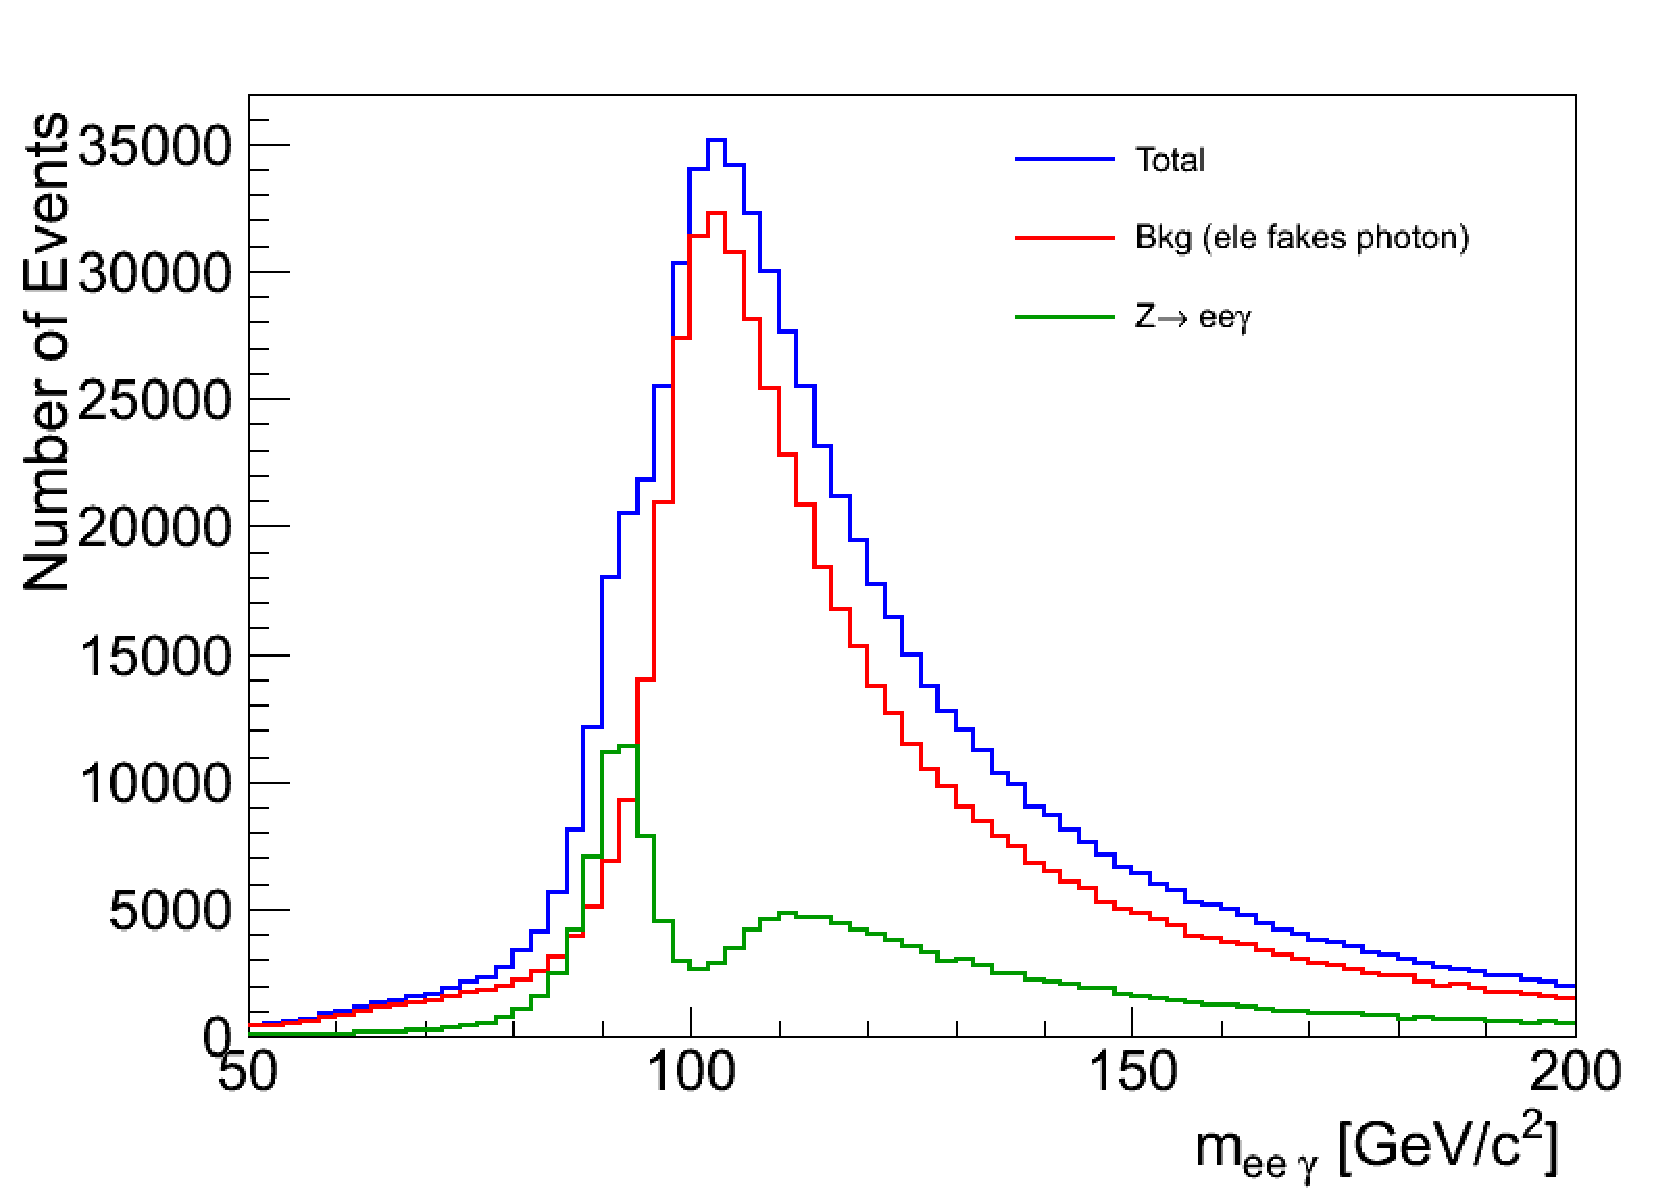
\includegraphics[width=0.6\textwidth]{figures/MassEEGamma_NoSelection.pdf}
    \caption{The distributions of the dielectron plus photon mass are shown for different processes. 
      The green histogram shows the $m_{ee\gamma}$ distribution for events where both electrons
      and the photon are real and promptly produced. The red histogram shows the $m_{ee\gamma}$ 
      distribution for events where at least one of the electrons or the photon was misidentified.
      The blue distribution shows the sum of the two different components.
    }
    \label{fig:MassEEGamma_NoSelection}
  \end{center}
\end{figure}

The distribution of $m_{ee\gamma}$ after the pixel seed veto requirement is shown in
Figure \ref{fig:MassEEGamma_AfterPixelVeto}. Next we make requirements on the 
dielectron mass and the sum of the dielectron mass and $m_{ee\gamma}$ to reduce
the background from initial state radiation, which does not represent a resonance peak
in $m_{ee\gamma}$ at the pole mass of the \Z\ boson. The distributions of $m_{ee}$
and $m_{ee} + m_{ee\gamma}$ are shown in Figure \ref{fig:ISRRemoval}. We require that
$m_{ee} + m_{ee\gamma} < 180$~\GeV\ and that $m_{ee} > 40$~\GeV. In addition,
to remain unbiased by the mass requirement in the tag and probe triggers, we require that
$m_{e\gamma} > 50$~\GeV.

\begin{figure}[htb]
  \begin{center}
    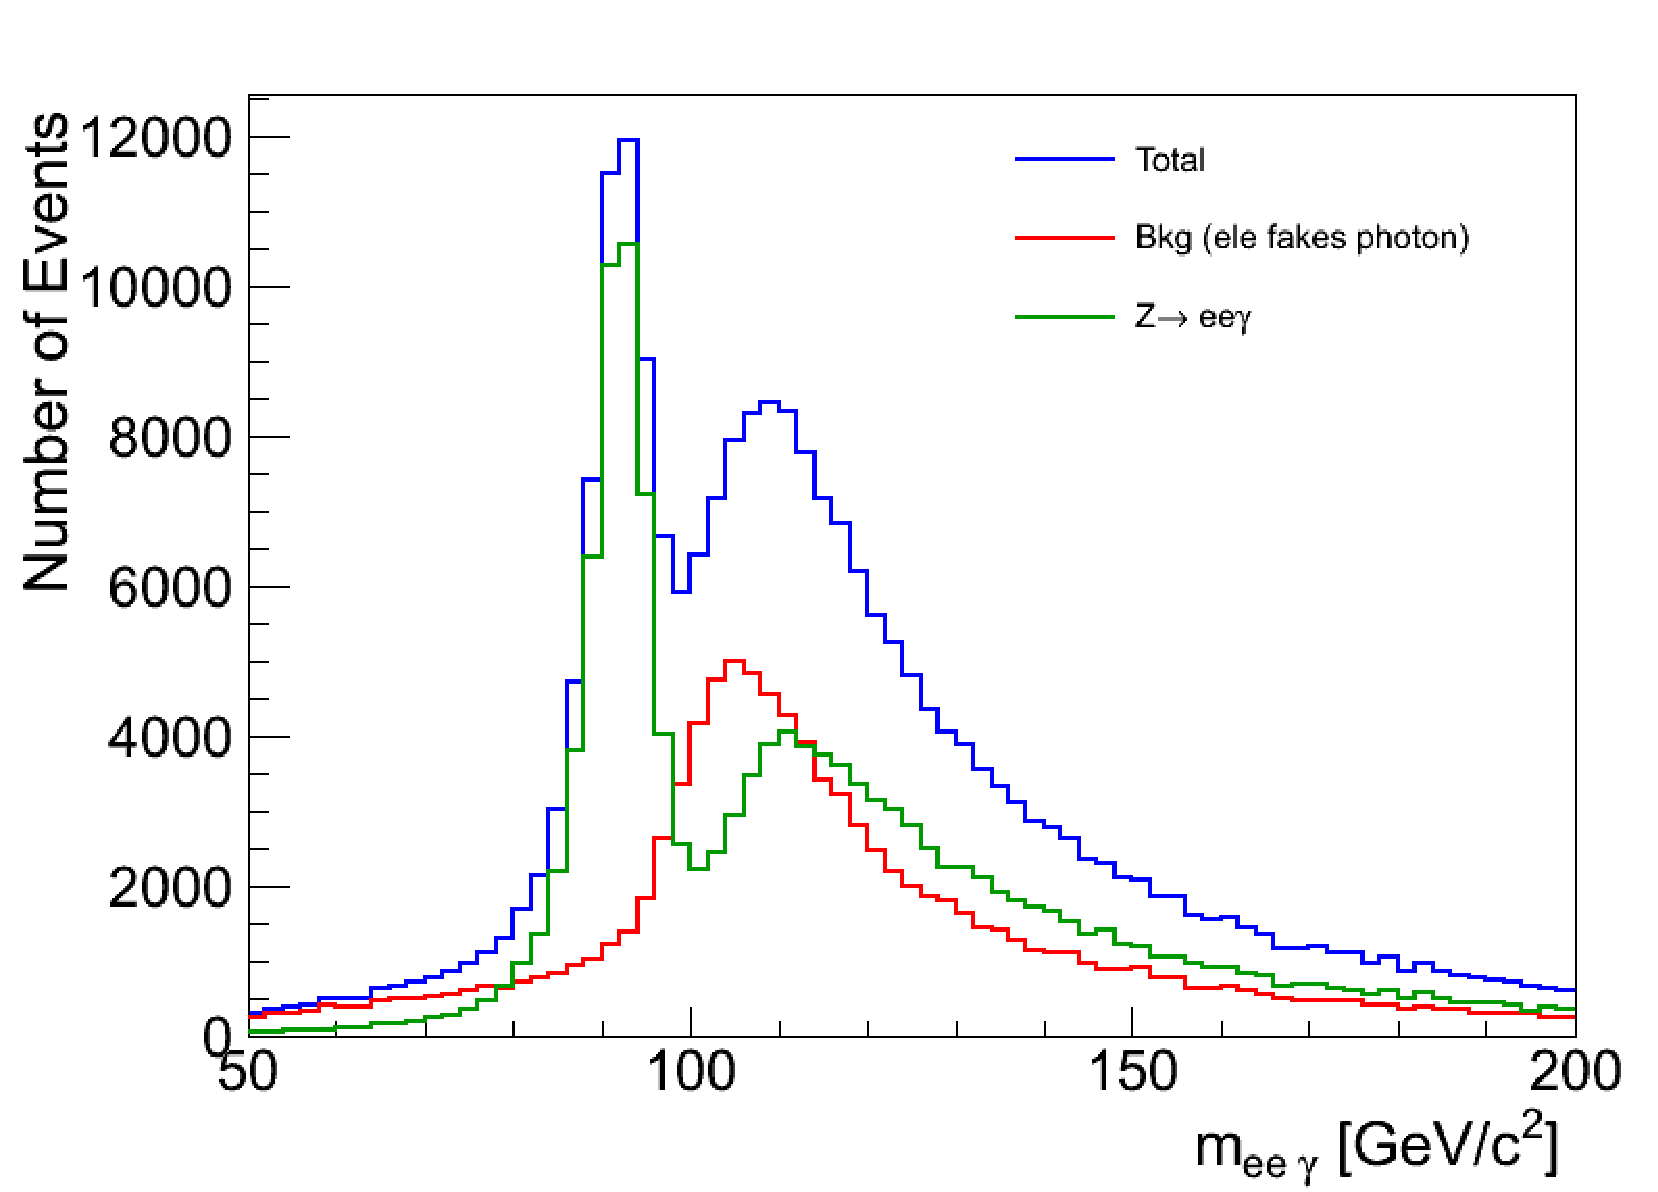
\includegraphics[width=0.6\textwidth]{figures/MassEEGamma_AfterPixelVeto.pdf}
    \caption{The distributions of $m_{ee\gamma}$ after the pixel seed veto requirement
      are shown for the different processes
      as described in the captions of Figure \ref{fig:MassEEGamma_NoSelection}.       
    }
    \label{fig:MassEEGamma_AfterPixelVeto}
  \end{center}
\end{figure}

\begin{figure}[htb]
  \begin{center}
    \subfigure[$m_{ee} + m_{ee\gamma}$]{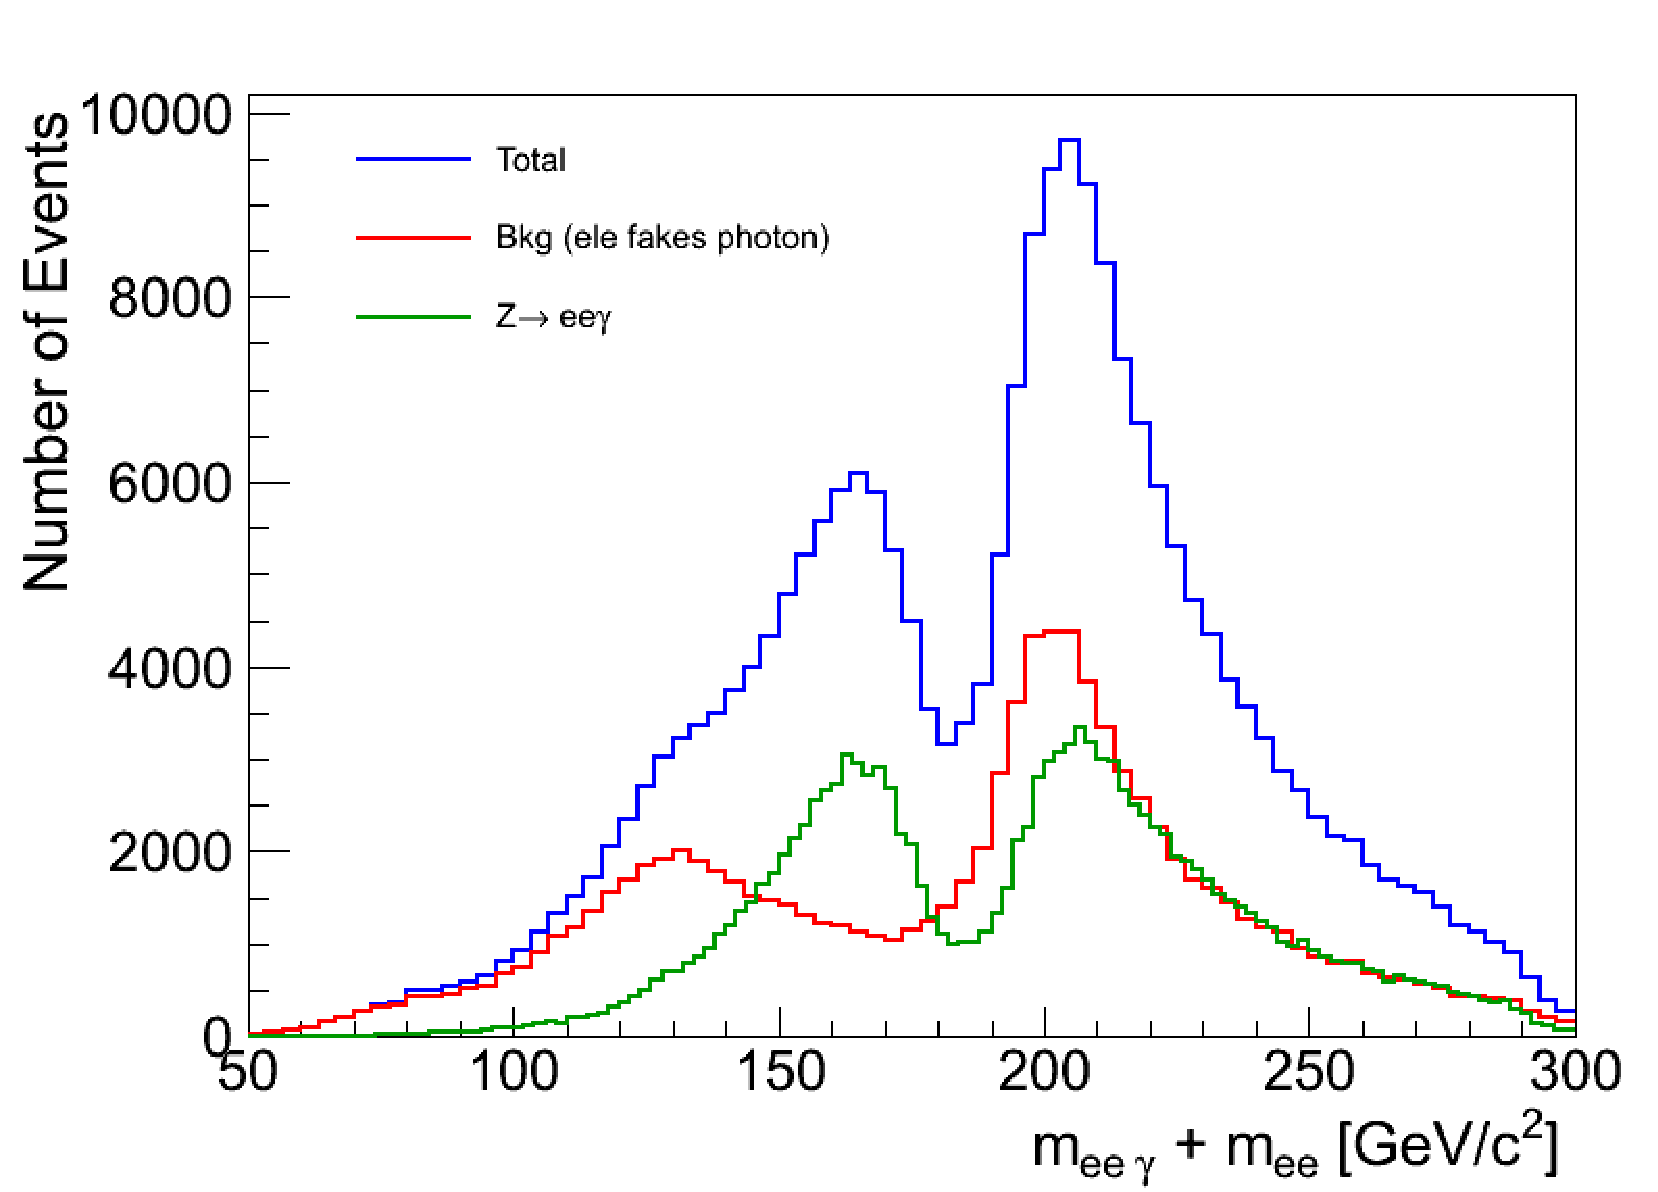
\includegraphics[width=0.48\textwidth]{figures/MassPlusDileptonmass_AfterPixelVeto.pdf}}
    \subfigure[$m_{ee}$]{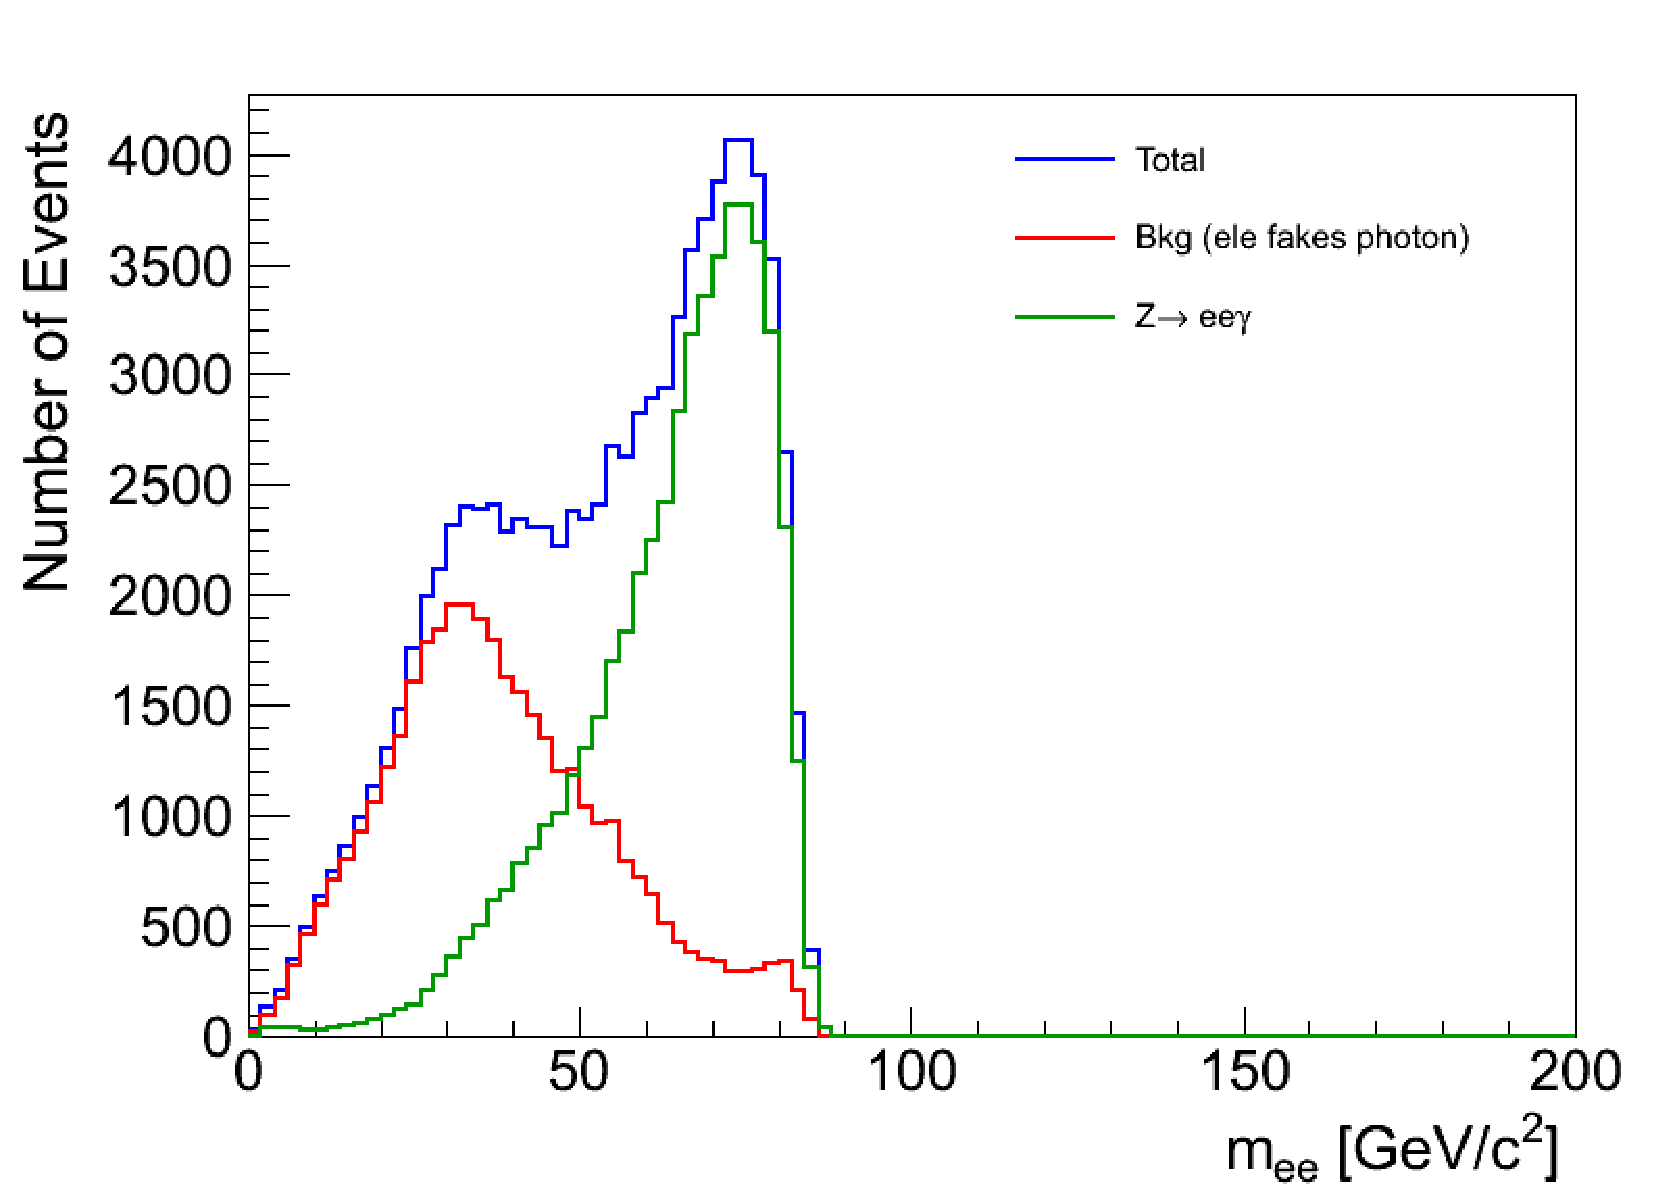
\includegraphics[width=0.48\textwidth]{figures/Dileptonmass_AfterISRRemoval.pdf}}
    \caption{ The distribution of the sum of the dielectron mass and $m_{ee\gamma}$ after the pixel seed veto
      requirement is shown in (a). The distribution of the dielectron mass after requiring that $m_{ee} + m_{ee\gamma} < 180$~\GeV\
      is shown in (b). 
    }
    \label{fig:ISRRemoval}
  \end{center}
\end{figure}

In Figure \ref{} we show the $m_{ee\gamma}$ distribution after these selection criteria 
that reduce the initial state radiation background for events where the probe has $p_{T}$ 
between $7$~\GeV\ and $10$~\GeV. At this stage, there are still a significant amount
of background remaining where the photon is a jet that has been misidentified. To reduce 
such backgrounds, we make more stringent requirements on the shower shape of the photon.
The distribution of $\mathrm{R}_{9}$ and $\sigma_{i\eta i\eta}$ are shown in 
Figures \ref{fig:PhotonR9_LowPtProbes} and \ref{fig:PhotonSigmaIEtaIEta_LowPtProbes} respectively. 
We require that the $\mathrm{R}_{9}$ is
larger than $0.9$ and that the $\sigma_{i\eta i\eta}$ is less than $0.0105$ and $0.028$ for
the barrel and endcap photons respectively. 

\begin{figure}[htb]
  \begin{center}
    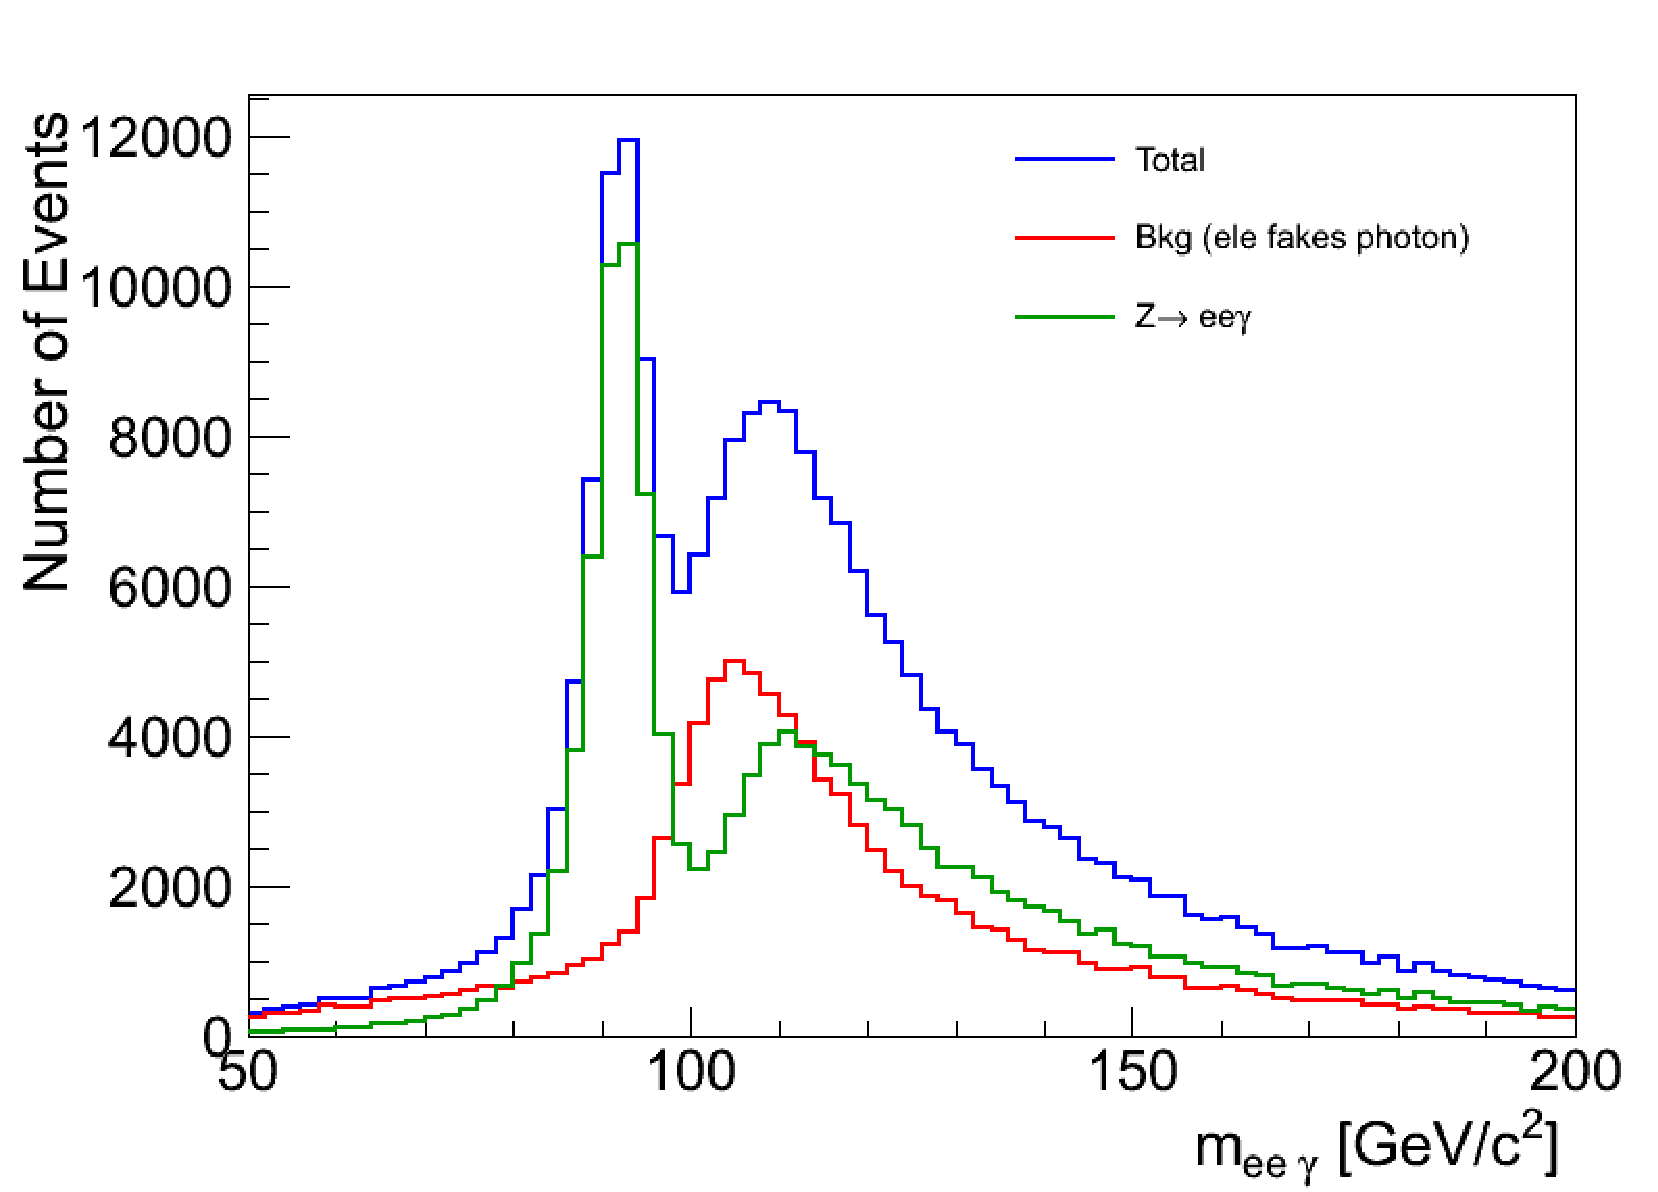
\includegraphics[width=0.6\textwidth]{figures/MassEEGamma_AfterPixelVeto.pdf}
    \caption{The distributions of $m_{ee\gamma}$ for events with probe electrons with $p_{T}$
      between $7$~\GeV\ and $10$~\GeV\ are shown.        
    }
    \label{fig:MassEEGamma_AfterPixelVeto}
  \end{center}
\end{figure}

\begin{figure}[htb]
  \begin{center}
    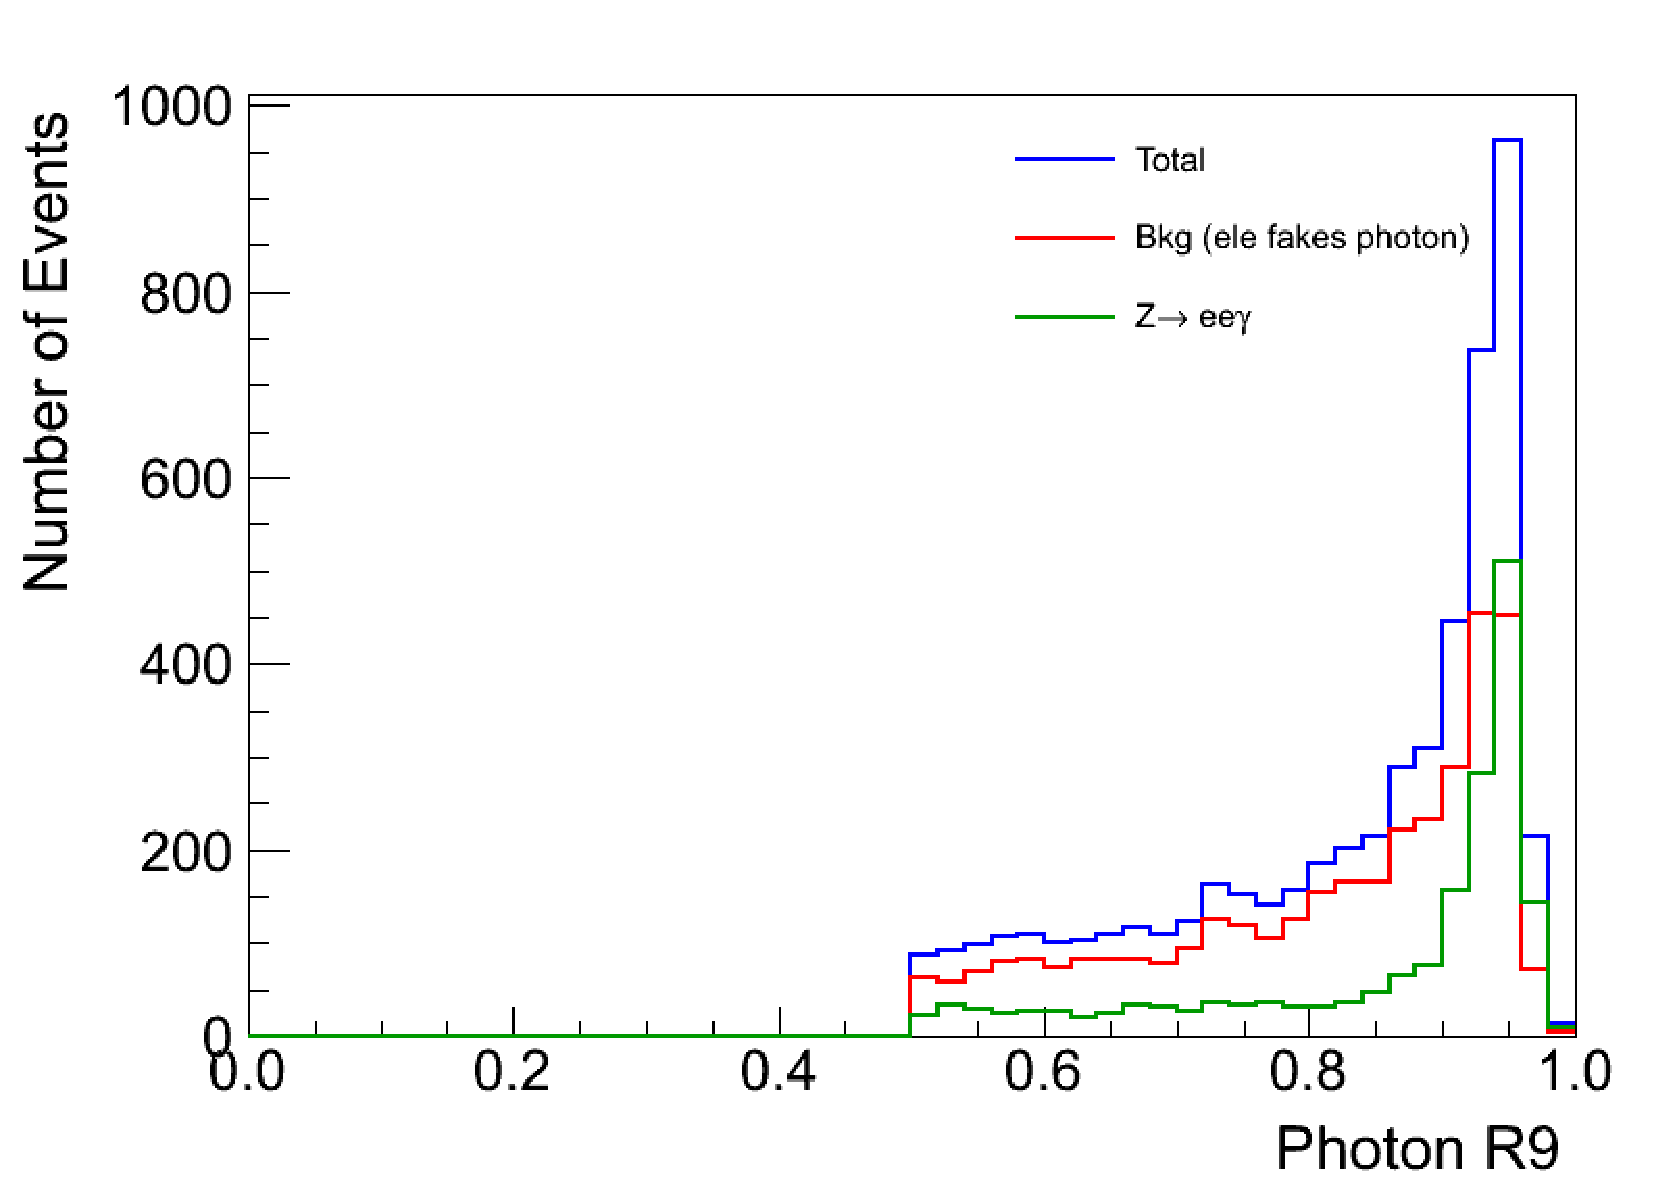
\includegraphics[width=0.6\textwidth]{figures/R9_AfterLowPtSelection.pdf}
    \caption{The distributions of the photon $\mathrm{R}_{9}$ for events with probe electrons with $p_{T}$
      between $7$~\GeV\ and $10$~\GeV\ are shown. 
    }
    \label{fig:PhotonR9_LowPtProbes}
  \end{center}
\end{figure}

\begin{figure}[htb]
  \begin{center}
    \subfigure[All Probes]{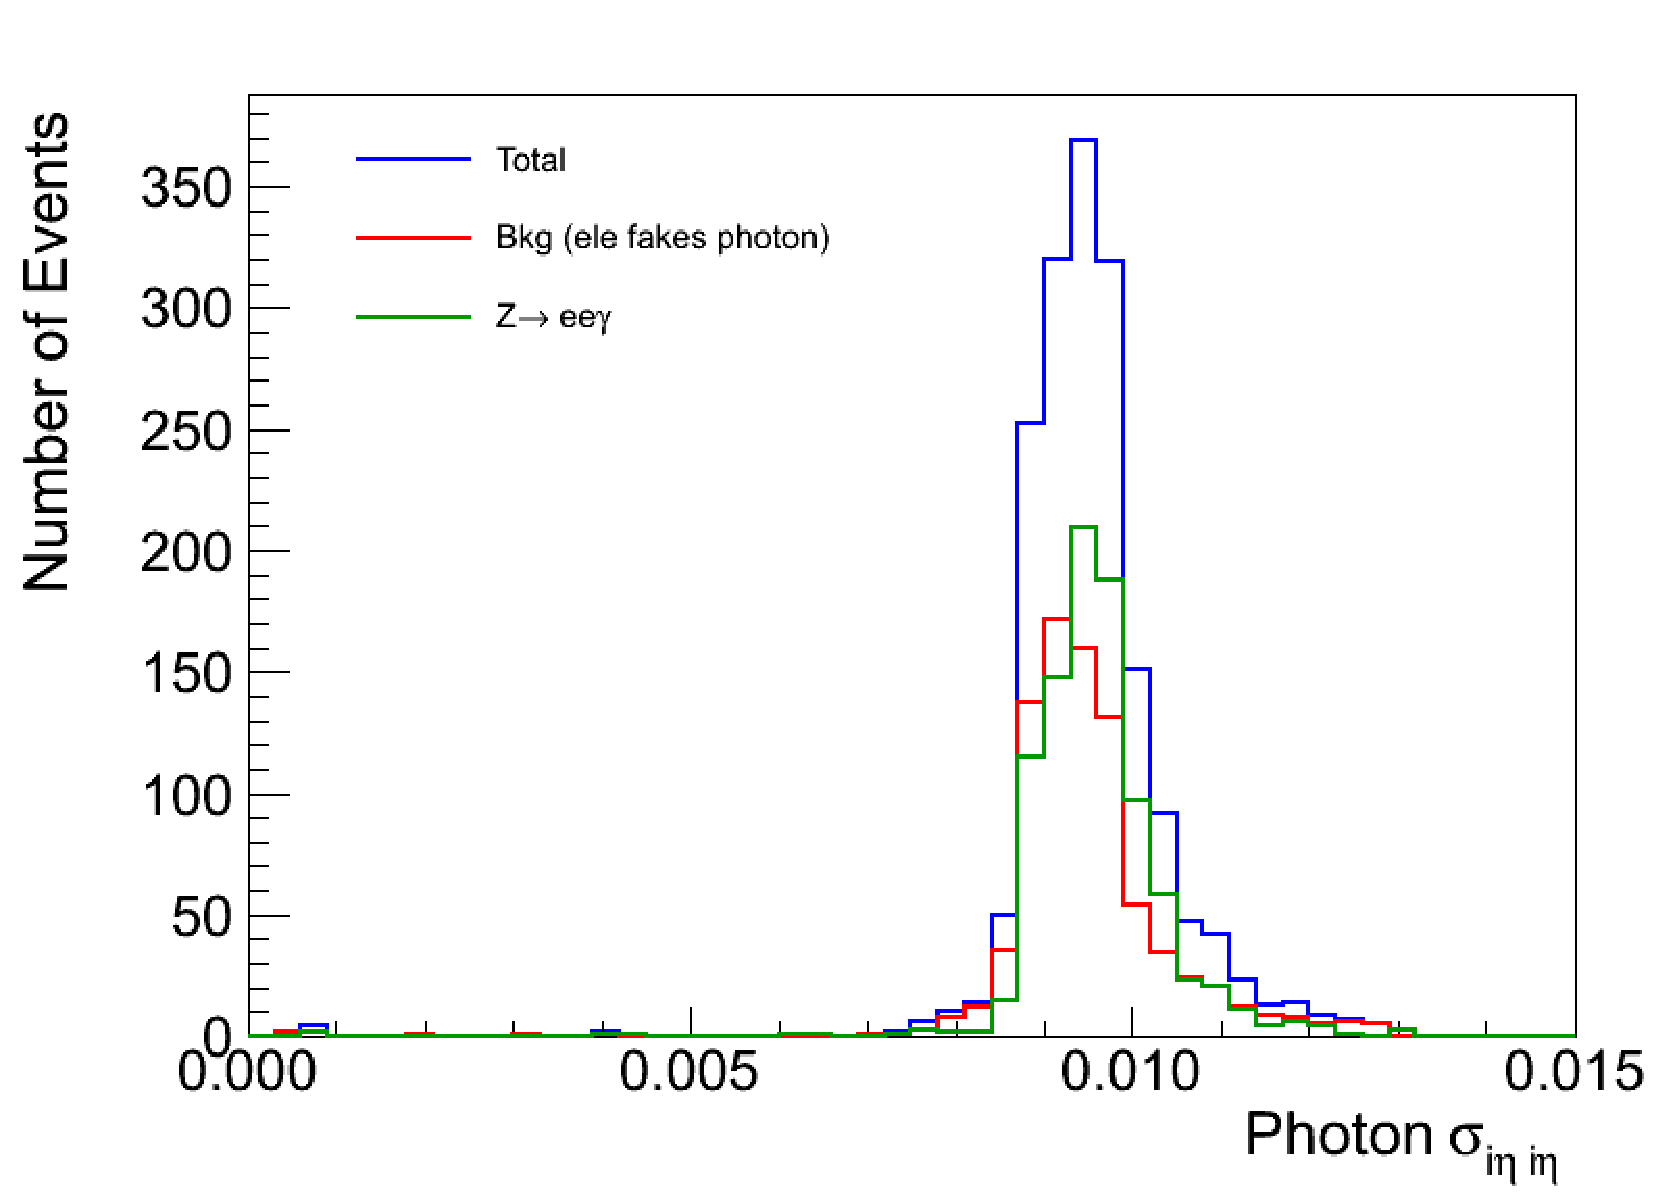
\includegraphics[width=0.48\textwidth]{figures/SigmaIEtaIEtaBarrel_AfterLowPtSelection.pdf}}
    \subfigure[Failing Probes]{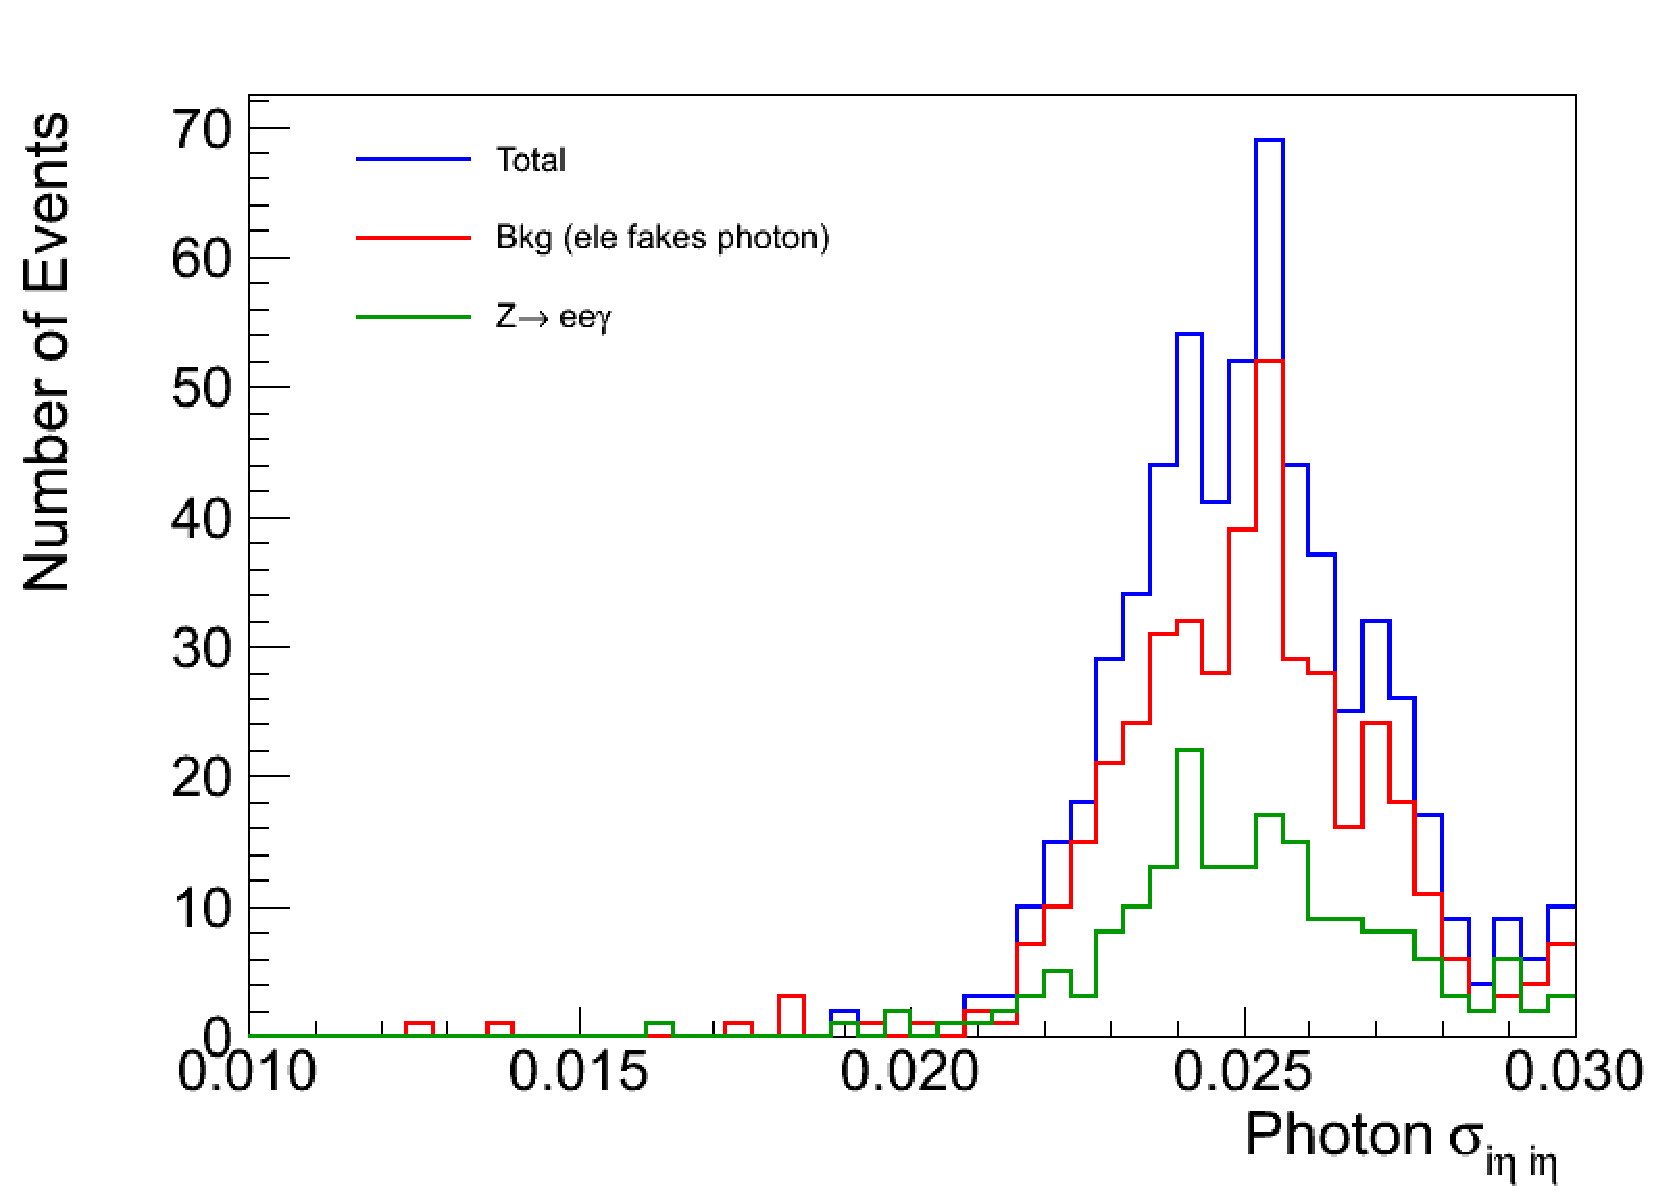
\includegraphics[width=0.48\textwidth]{figures/SigmaIEtaIEtaEndcap_AfterLowPtSelection.pdf}}
    \caption{ The distributions of the photon $\sigma_{i\eta i\eta}$ for events with probe electrons with $p_{T}$
      between $7$~\GeV\ and $10$~\GeV\ are shown. 
    }
    \label{fig:PhotonSigmaIEtaIEta_LowPtProbes}
  \end{center}
\end{figure} 


Finally, the signal to background can be significantly enhanced by requiring that the photon and the probe 
electron are geometrically near each other. The distribution of the $\Delta$R between the photon and the
probe electron is shown in Figure \ref{fig:DeltaRProbePhoton}. We require that the $\Delta$R is less
than $0.7$. After making all of these selection requirements, we obtain the $m_{ee\gamma}$ distribution
shown in Figure \ref{fig:MassEEGamma_AfterAllSelection}. The signal to background in the region near the 
pole mass of the \Z\ boson is better than $10:1$. 

\begin{figure}[htb]
  \begin{center}
    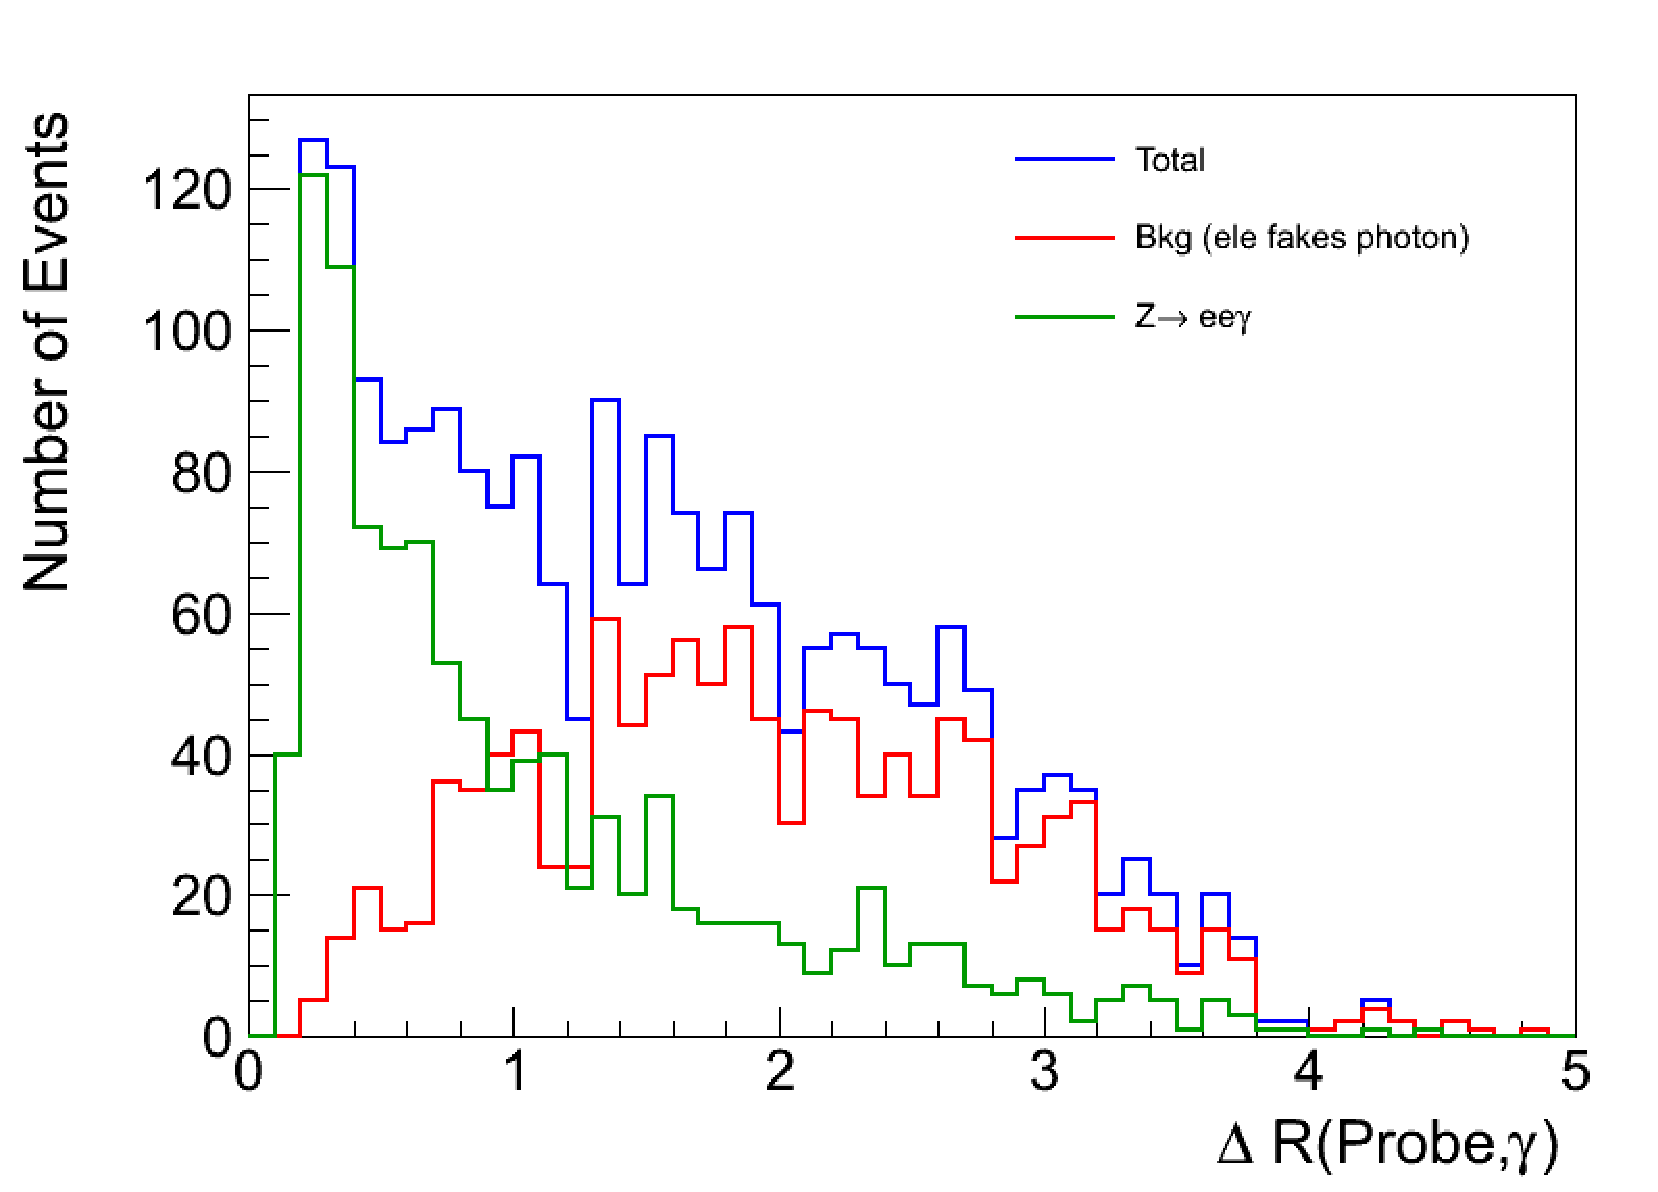
\includegraphics[width=0.6\textwidth]{figures/DeltaRProbePhoton_AfterPhotonSelection.pdf}
    \caption{The distributions of $\Delta$R between the photon and the probe electron,
      for events with probe electrons with $p_{T}$ between $7$~\GeV\ and $10$~\GeV
    }
    \label{fig:DeltaRProbePhoton}
  \end{center}
\end{figure}

\begin{figure}[htb]
  \begin{center}
    \subfigure[Barrel]{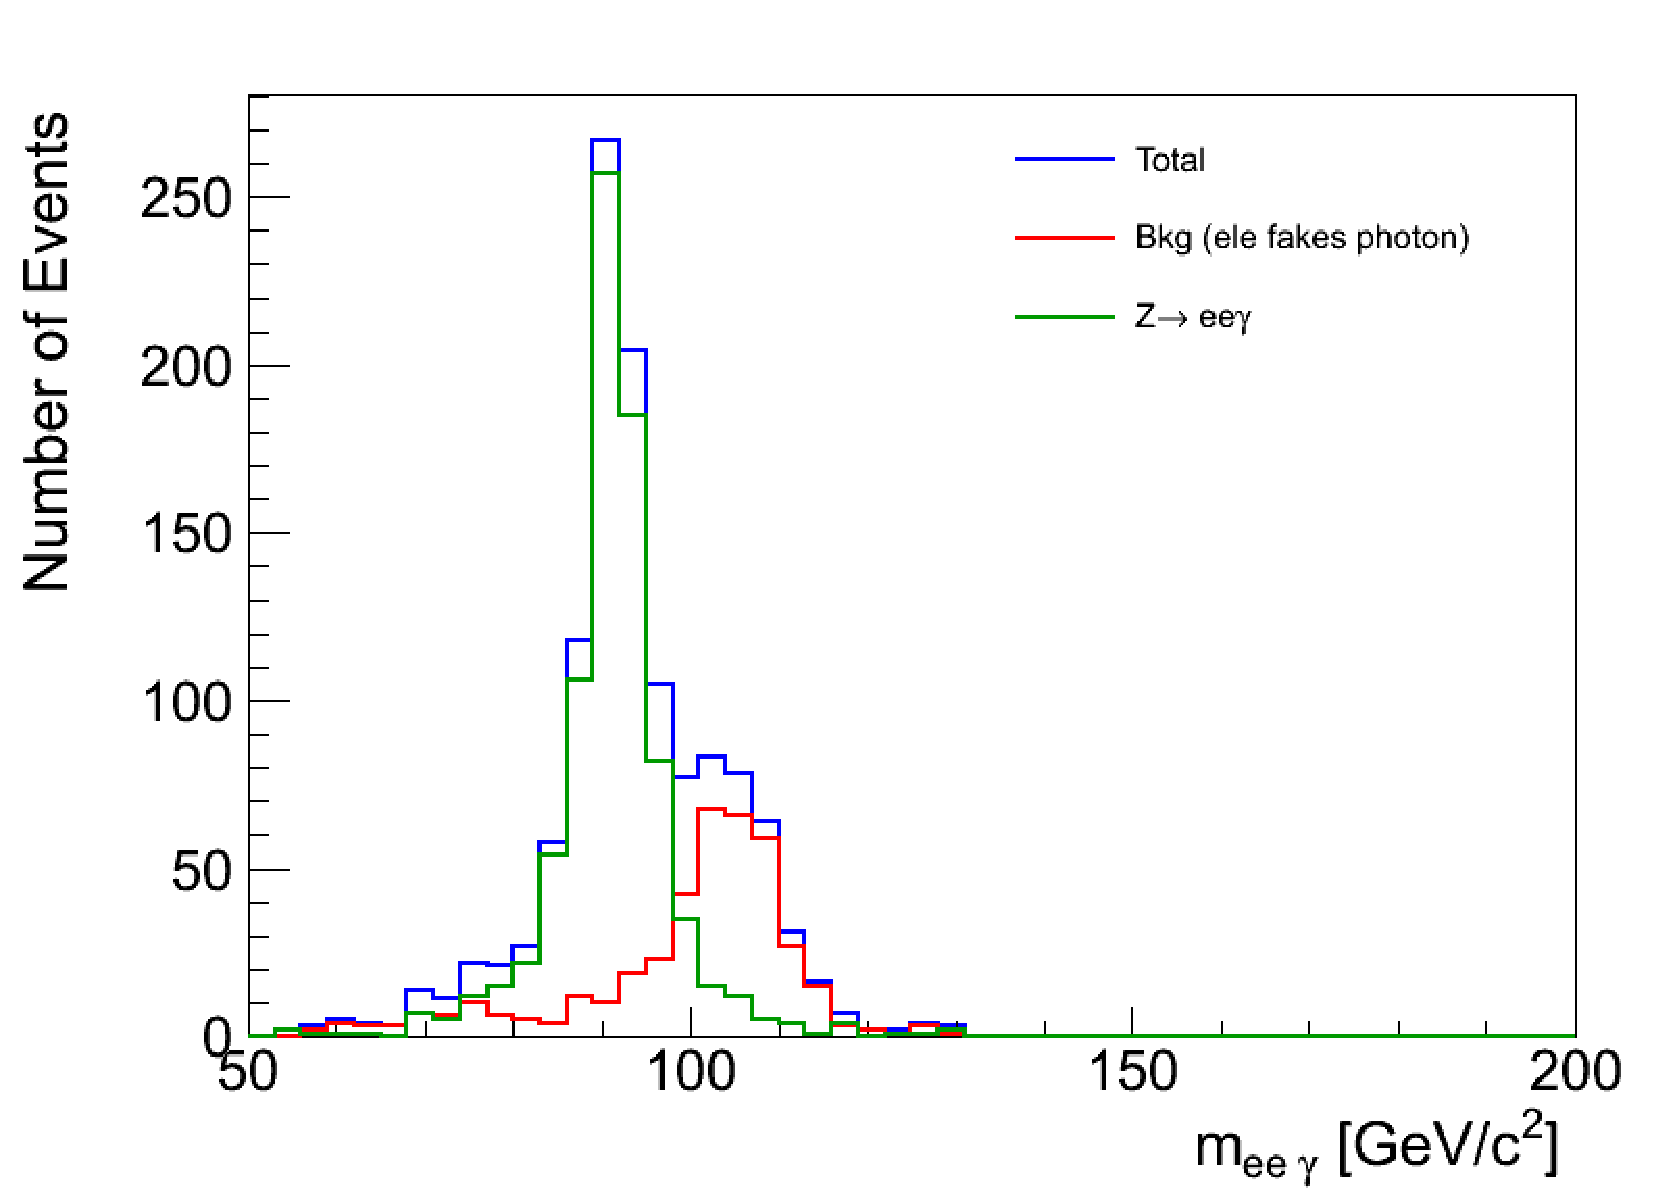
\includegraphics[width=0.48\textwidth]{figures/MassEEGamma_AfterAllSelection.pdf}}
    \subfigure[Endcap]{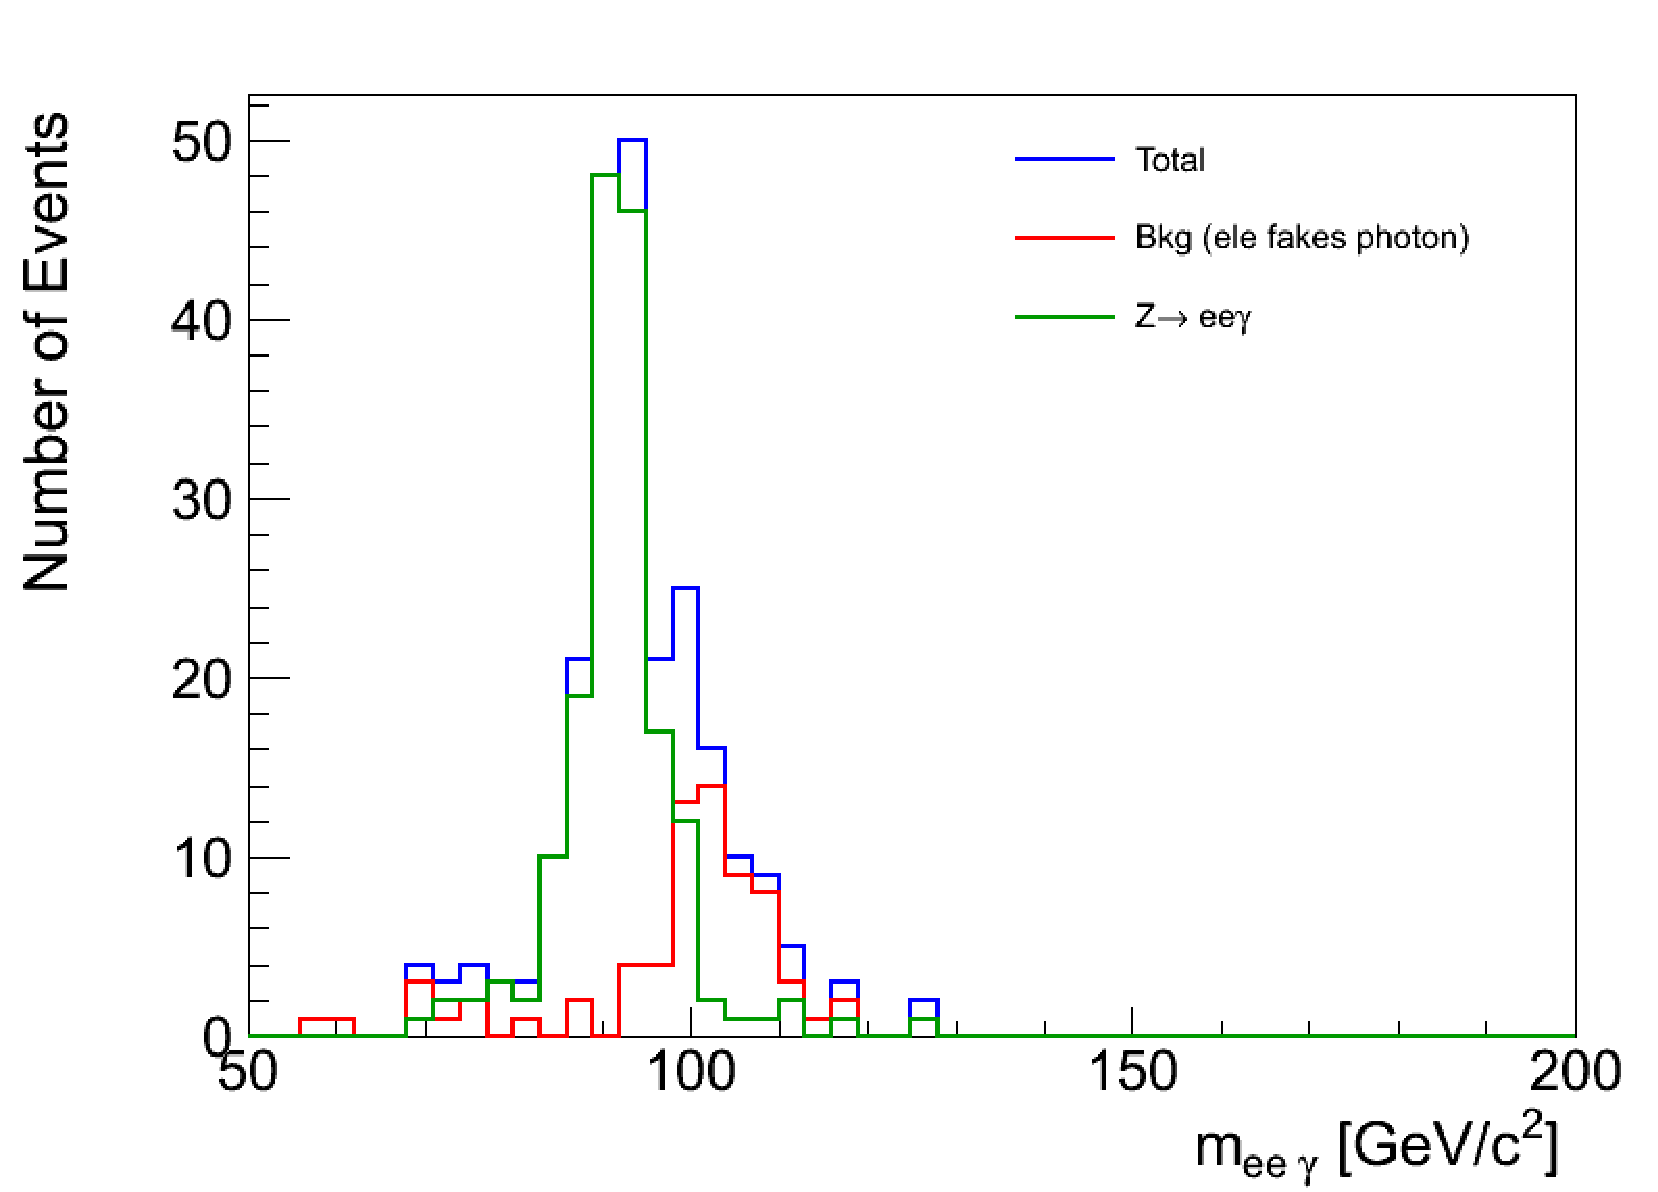
\includegraphics[width=0.48\textwidth]{figures/MassEEGamma_AfterAllSelectionProbeFail.pdf}}
    \caption{The distributions of $m_{ee\gamma}$ after all selection requirements
      for events with probe electrons with $p_{T}$ between $7$~\GeV\ and $10$~\GeV\  are shown. 
      All such events are shown in (a), and those events where the probe electron fails the 
      selection requirements used for the \HiggsToZZ\ analysis are shown in (b). 
    }
    \label{fig:MassEEGamma_AfterAllSelection}
  \end{center}
\end{figure}


\subsection{ Efficiency Fit Models }

To extract the efficiency we perform a simultaneous unbinned maximum likelihood fit of the $m_{ee\gamma}$ mass 
distribution for events where the probe passes the particular selection requirement and the events where 
the probe fails the particular selection requirements. The shape of the signal in $m_{ee\gamma}$ is 
modelled by the convolution of the template shape obtained from the simulation with a gaussian whose 
mean and width are allowed to float. The gaussian is intended to model any potential difference in
the energy scale and resolution of the electrons and photon between the simulation and the data. 

From Figure \ref{fig:MassEEGamma_AfterAllSelection} one can see that the background is dominated by events
where one of the electrons from the \Z\ boson decay is misidentified as a photon, and the probe electron
is a jet that has been misidentified. This event sample exhibits a particular $m_{ee\gamma}$ shape which is
primarily determined by the kinematics of the event. The fact that the tag electron and photon system originate
from the \Z\ boson resonance and the fact that the probe electron is required to have $p_{T}$ around $10$~\GeV\ 
implies that the shape of the $m_{ee\gamma}$ will exhibit a peaking structure slightly
above $100$~\GeV. Since the shape of this distribution is primarily determined by kinematics, the simulation
prediction is expected to the fairly accurate. In particular the separation in the peak between this background
and the final state radiation signal predicted by the Monte Carlo simulation is expected to be quite robust. 
Therefore, we model the shape of the background with a convolution of the same gaussian as defined above for the 
signal and the template shape obtained for the background from the simulation. Finally another exponential
background component is added to describe the contribution from any remaining processes, which are expected to be
very small. The use of the convolution with the same gaussian function for signal and background essentially
corrects for an overall energy scale and resolution, but assumes that these corrections do not differ between
the signal and the background. Given that the signal and background are very similar, one exhibiting a peak at the
pole mass of the \Z\ boson and one exhibiting a peak about $10$~\GeV\ higher, the assumption that the energy
scale and resolution corrections from the simulation to the data is the same is a fairly robust one. 

Due to the fact that the simulation has a limited number of events passing all selection cuts, the 
background template will exhibit significant statistical fluctuations. To partially mitigate this problem,
we note that the shape of the $m_{ee\gamma}$ distribution for background does not have any significant 
dependence on the $\Delta$R. This is illustrated in Figure \ref{fig:BackgroundShapeModeling}, where we 
observe that the shape is identical for events with $\Delta$R$<0.7$ and events 
with $0.7 < \Delta$R$<1.5$. Beyond $1.5$, the shape begins to exhibit small biases. 
Therefore we use events with $\Delta$R$<1.5$ from the simulation to build the mass shape templates. 
Furthermore, for the background, variation in the $m_{ee\gamma}$ distribution shape
between the barrel and the endcap is small compared to statistical fluctuations of the 
Monte Carlo sample. Therefore, we combine the barrel and endcap templates to suppress
the effect of statistical fluctuations of the limited Monte Carlo sample. This is observed to yield
more stable fit results.


\begin{figure}[htb]
  \begin{center}
    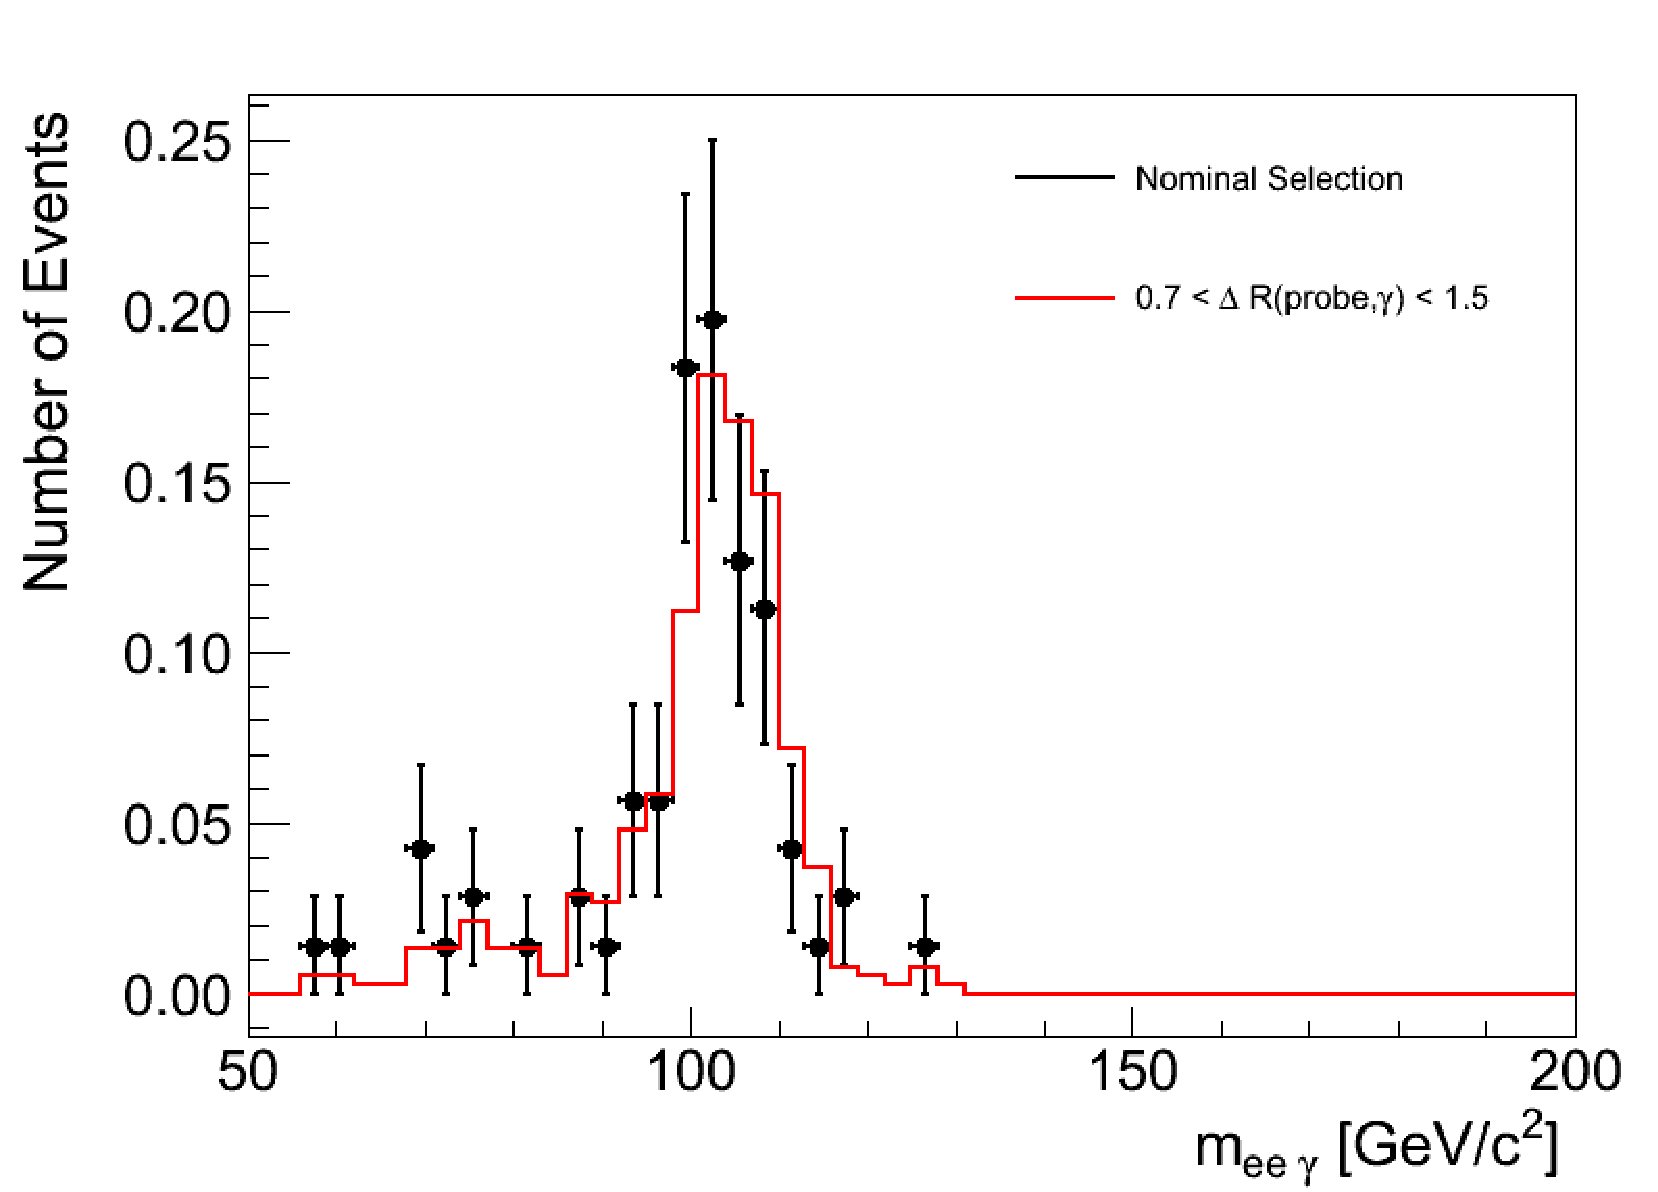
\includegraphics[width=0.6\textwidth]{figures/MassEEGamma_BackgroundShapeModeling.pdf}
    \caption{A comparison of the $m_{ee\gamma}$ shape is shown between events with $\Delta$R$<0.7$ and events 
      with $0.7 < \Delta$R$<1.5$ for the background.
    }
    \label{fig:BackgroundShapeModeling}
  \end{center}
\end{figure}

\subsection{ Photon Footprint Removal }

For the measurement of the isolation efficiency, it is very important to properly account for the footprint
of the photon near the probe. We must properly match the photon to the corresponding particle flow candidate
in the isolation cone of the probe electron, and exclude it from the isolation sum. Ideally this matching
can be done using the reference from the photon and the particle flow candidate to the same supercluster
object. For technical reasons, we perform this matching by excluding any particle flow photons with 
$|\Delta\eta|<0.015$ to the reconstructed photon if the photon is in the barrel, and excluding any particle
flow photons with $\Delta$R$<0.07$ to the reconstructed photon if the photon is in the endcap. Furthermore,
we exclude the particle flow candidate of any type with the smallest $\Delta$R to the reconstructed
photon is the $\Delta$R is less than $0.1$. After performing this footprint removal, we obtain a fairly
flat efficiency as a function of the $\Delta$R between the photon and the probe electron. This efficiency 
measured from the simulation is shown in Figure \ref{fig:EfficiencyVsDeltaR}.

\begin{figure}[htb]
  \begin{center}
    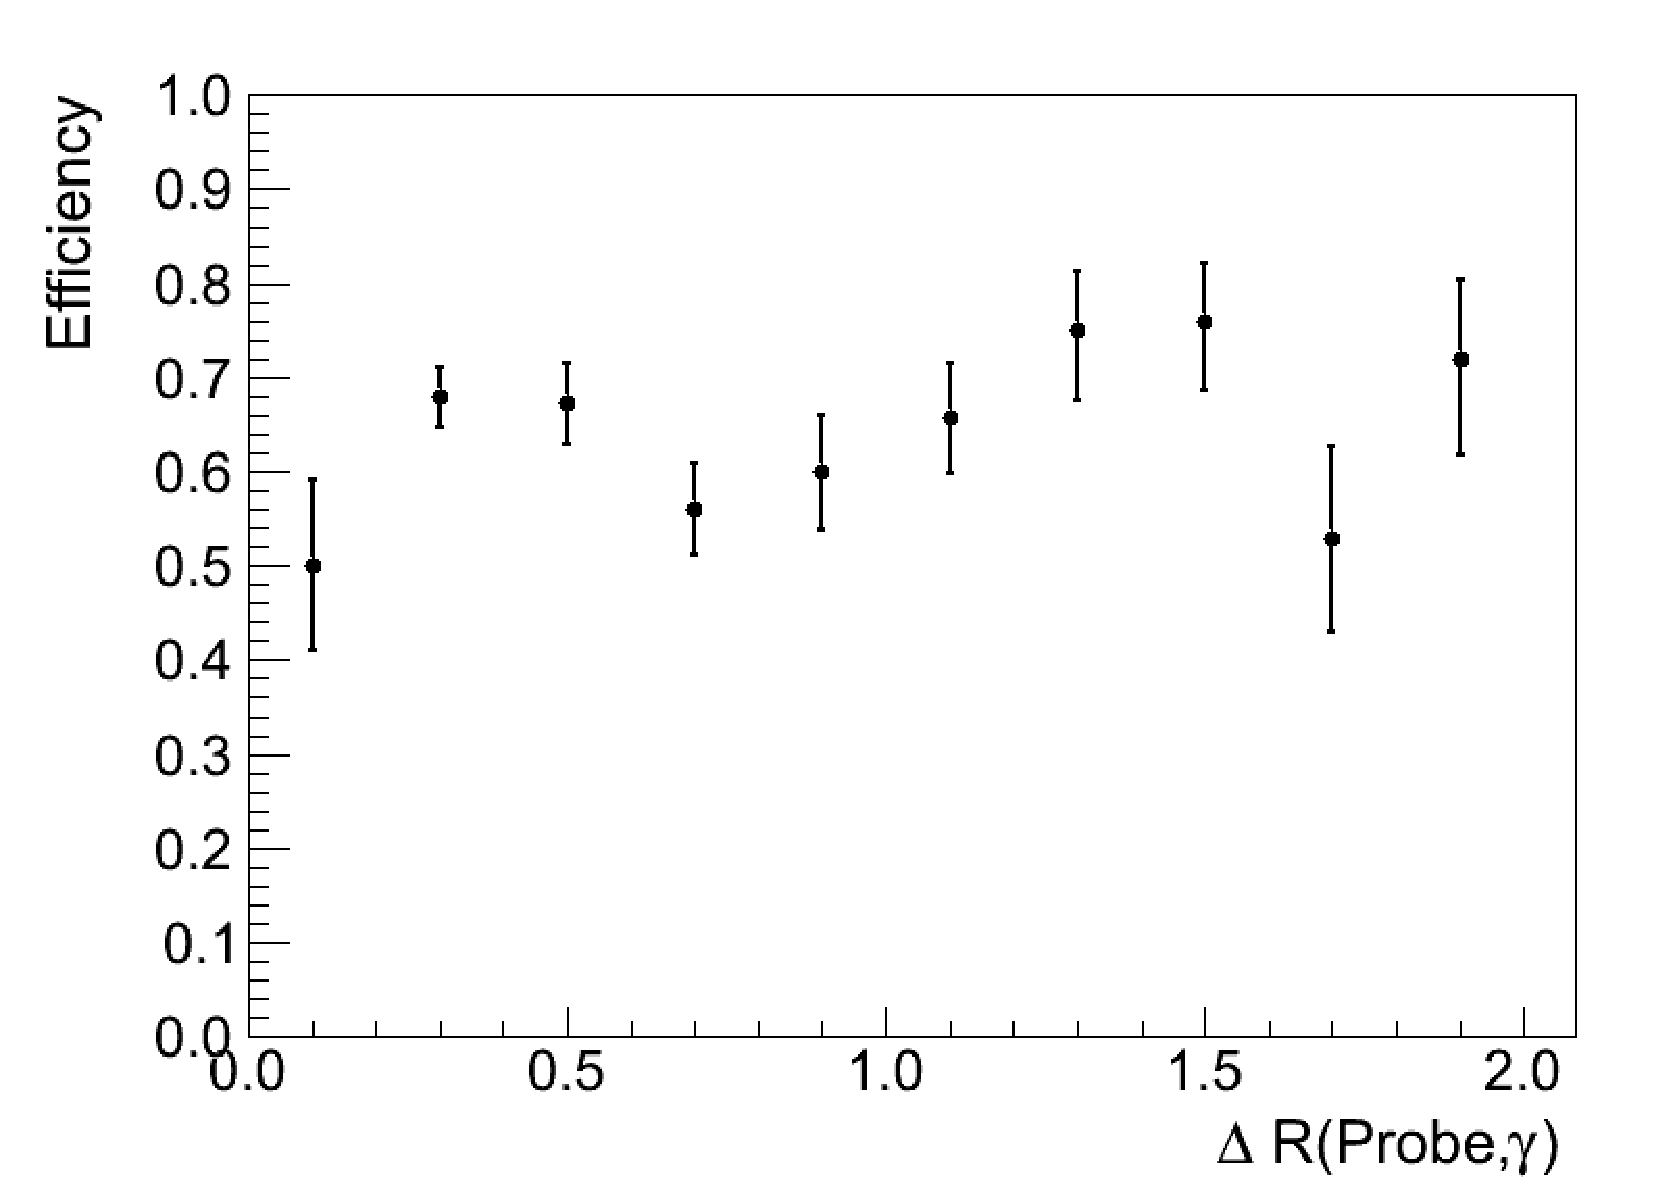
\includegraphics[width=0.6\textwidth]{figures/Efficiency_DeltaRProbePhoton.pdf}
    \caption{The efficiency of the electron selection used for the \HiggsToZZ\ analysis for ICHEP 2012 for
      probe electrons with $p_{T}$ between $7$~\GeV\ and $10$~\GeV, as a function of the $\Delta$R between
      the photon and the probe electron.
    }
    \label{fig:EfficiencyVsDeltaR}
  \end{center}
\end{figure}


\section{Results}

Using the method described above, we measure the efficiency for reconstructed GSF electrons to pass the 
selection cuts used for the ICHEP 2012 \HiggsToZZ\ analysis \cite{HZZICHEPCMSNote,HZZICHEPCaliforniaCMSNote}.
The result of the efficiency extraction fits are shown in Figures \ref{fig:MassFits_Pt7To10}, \ref{fig:MassFits_Pt10To15},
and \ref{fig:MassFits_Pt15To20} for electrons with $p_{T}$ between $7$~\GeV\ and $10$~\GeV, between $10$~\GeV\ and $15$~\GeV,
and between $15$~\GeV\ and $20$~\GeV respectively. Since the background in the passing sample are negligibly small, we
fixed the background to zero in the fit for the pass sample.  
The efficiency measured from the Monte Carlo simulation, the data, and the
Monte Carlo to data scale factors are summarized in bins of $p_{T}$ and $\eta$ in Table \ref{tab:Efficiency_HZZICHEP2012WP}.
We observe that the scale factors are consistent with $1.0$ for the bins with $p_{T}$ between $10$~\GeV\ and $20$~\GeV.
For the lowest $p_{T}$ bin, the scale factor is about $0.8$ in the barrel and $0.7$ in the endcap. 

\begin{figure}[htb]
  \begin{center}
    \subfigure[Barrel Pass]{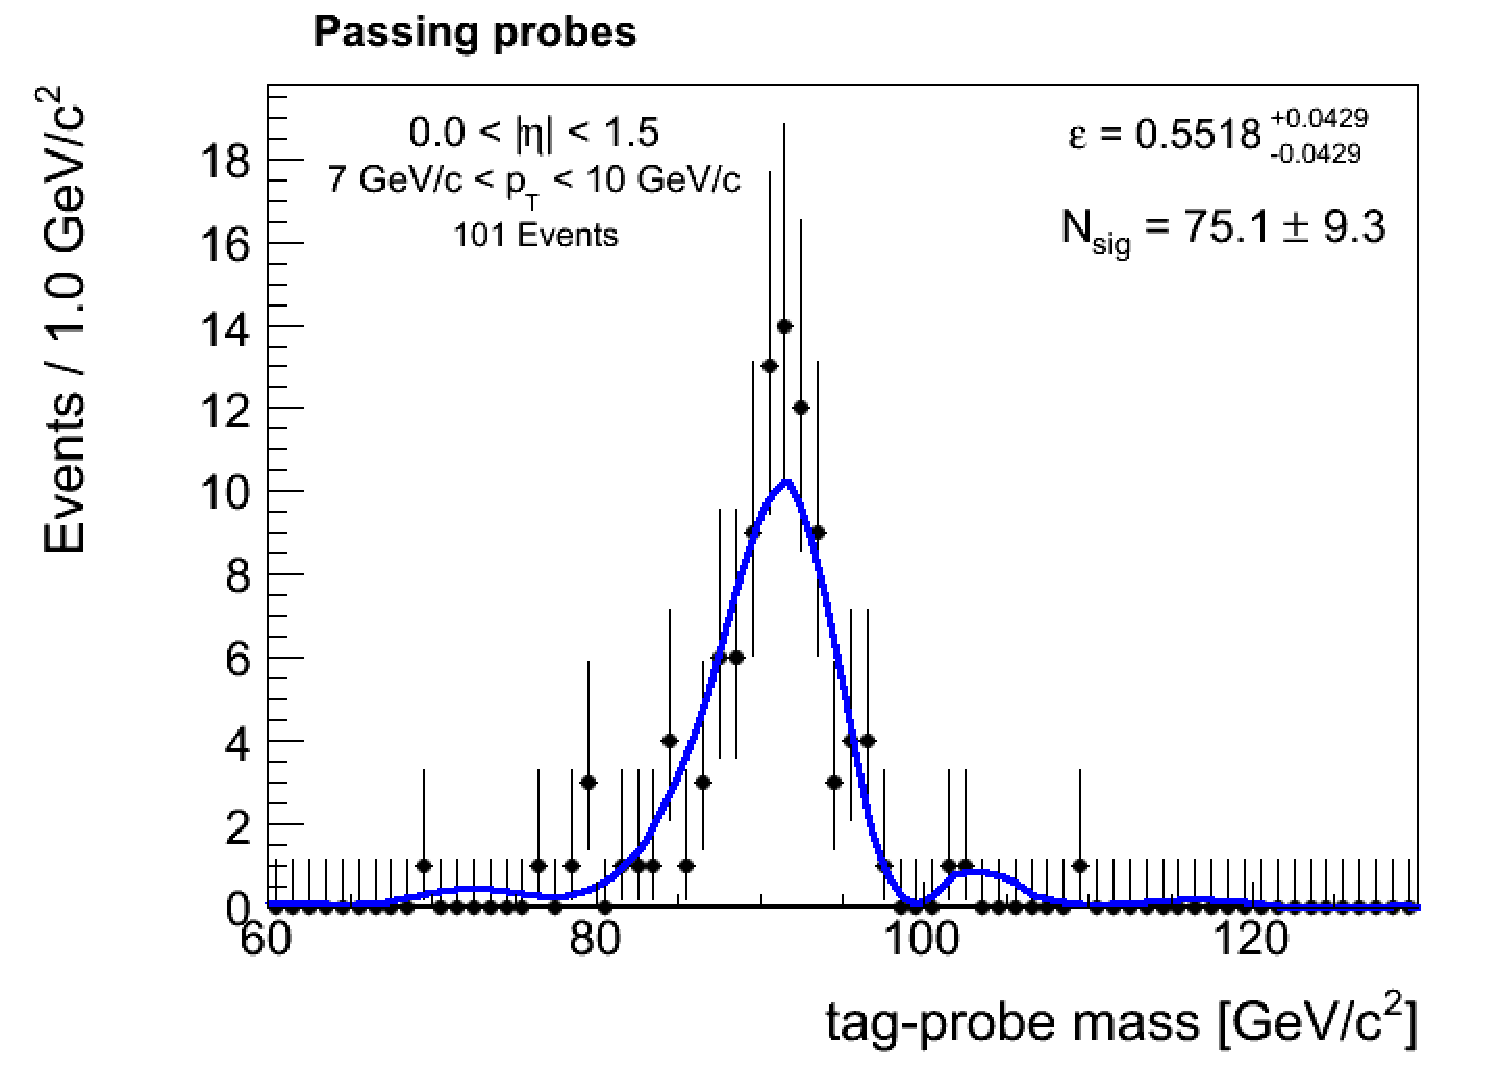
\includegraphics[width=0.48\textwidth]{figures/passetapt_TemplateConvGausPlusExpFit_0.pdf}}
    \subfigure[Barrel Fail]{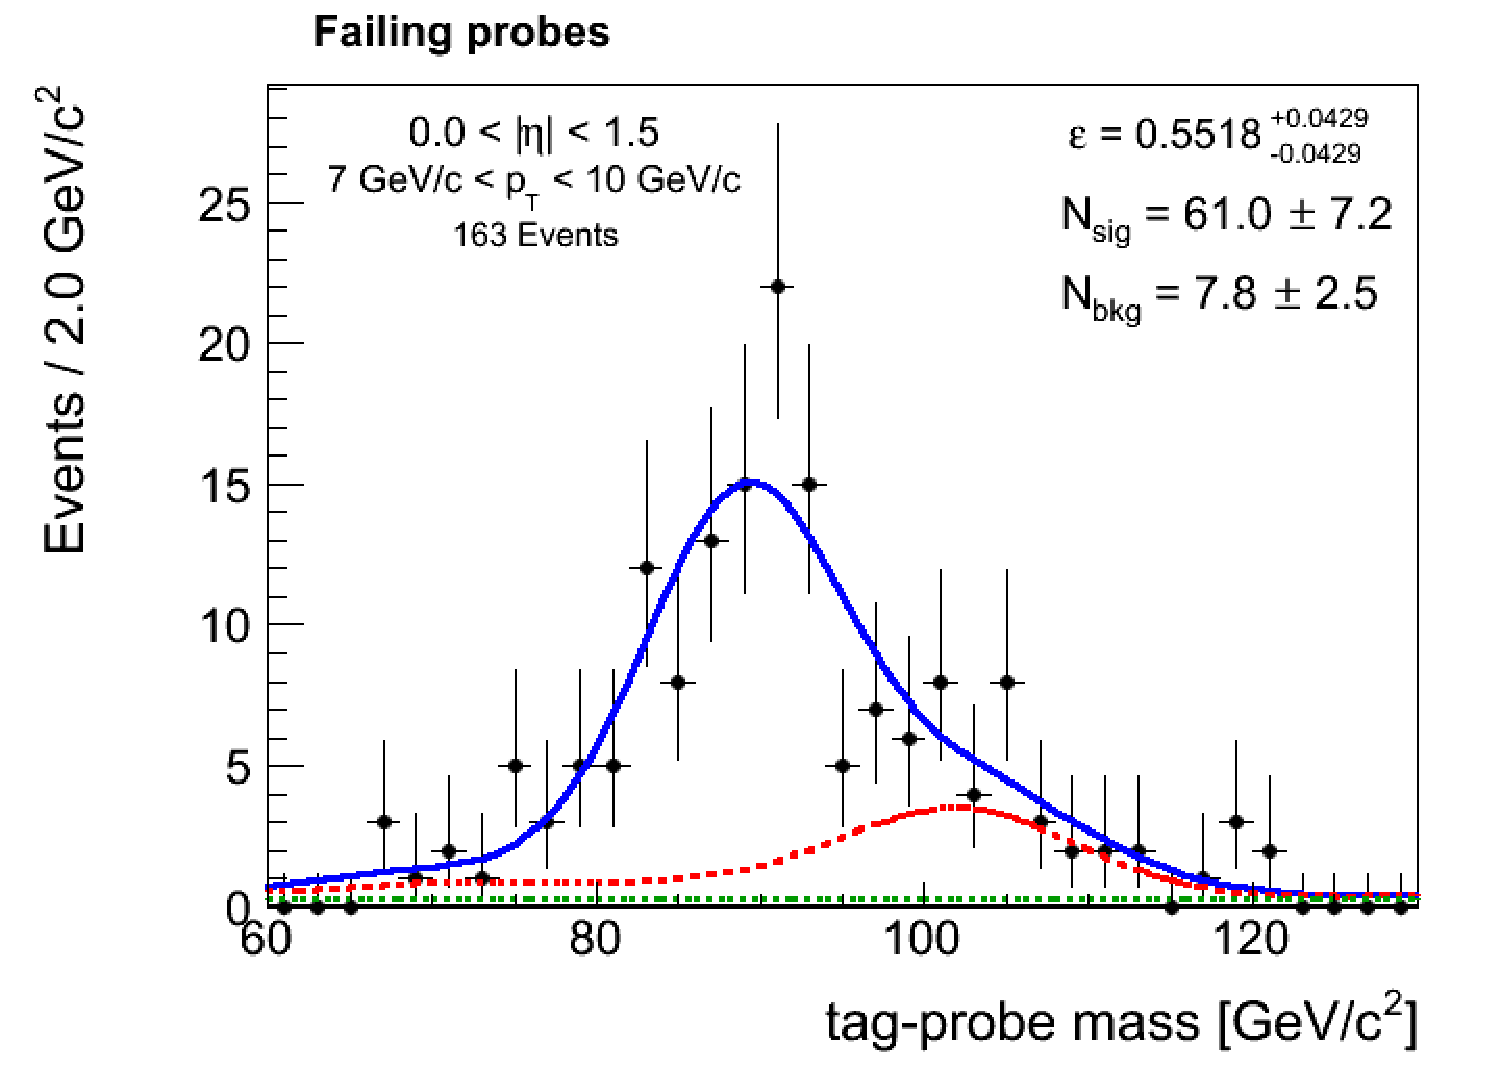
\includegraphics[width=0.48\textwidth]{figures/failetapt_TemplateConvGausPlusExpFit_0.pdf}}
    \subfigure[Endcap Pass]{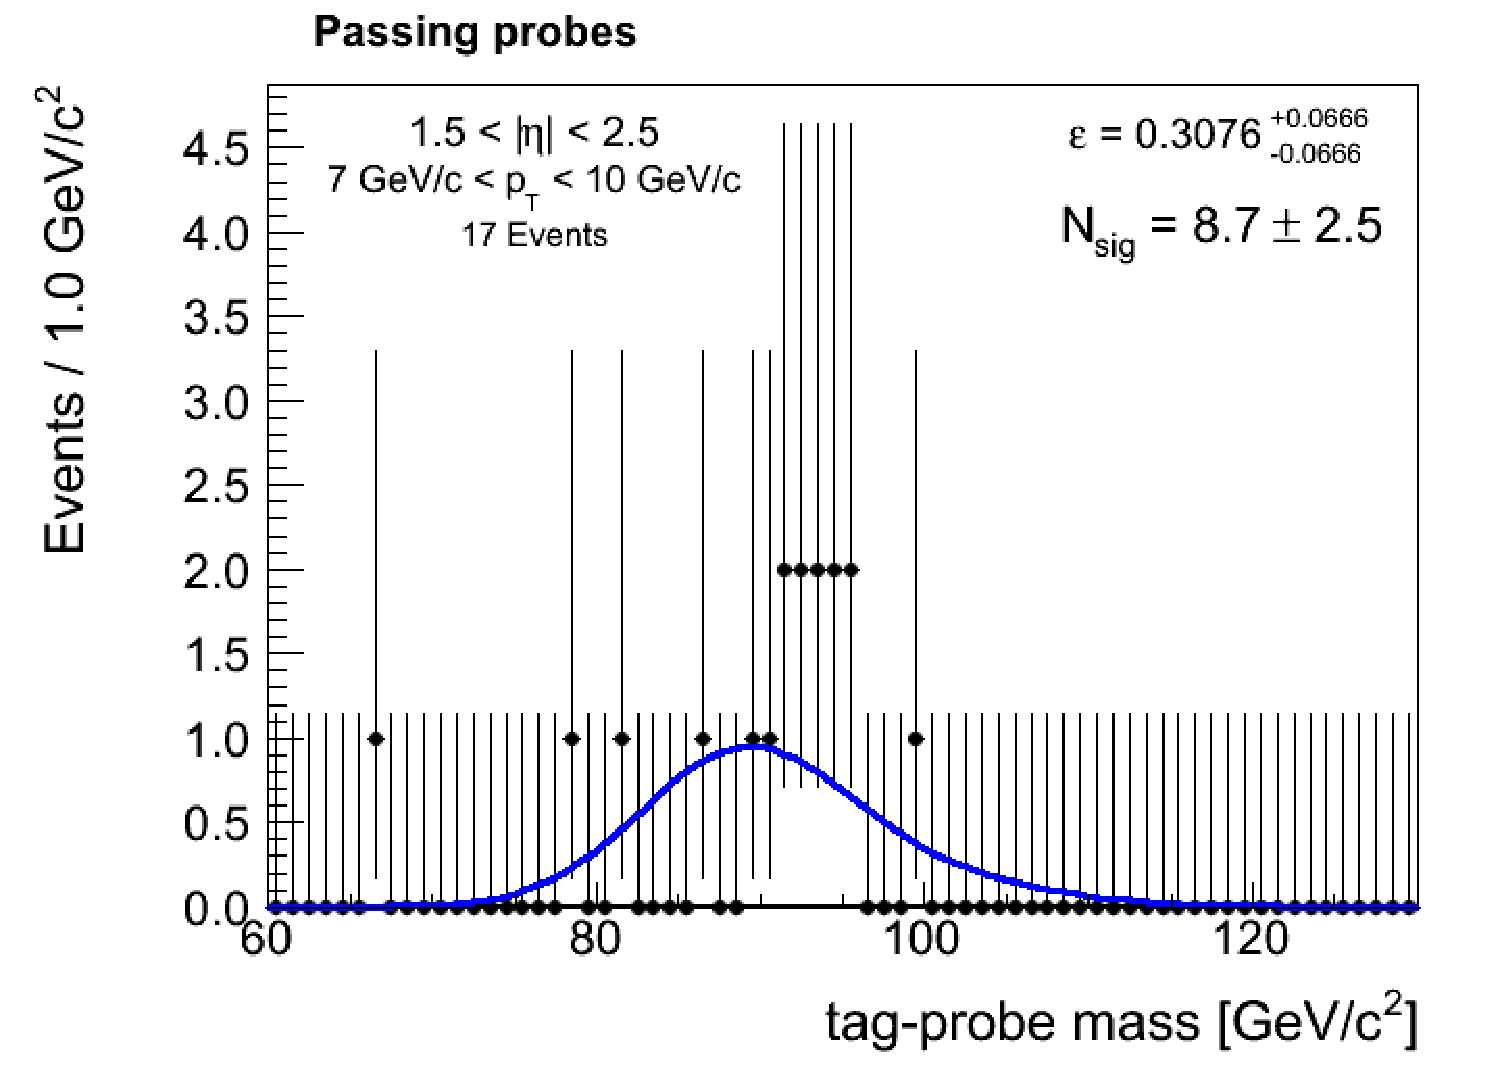
\includegraphics[width=0.48\textwidth]{figures/passetapt_TemplateConvGausPlusExpFit_1.pdf}}
    \subfigure[Endcap Fail]{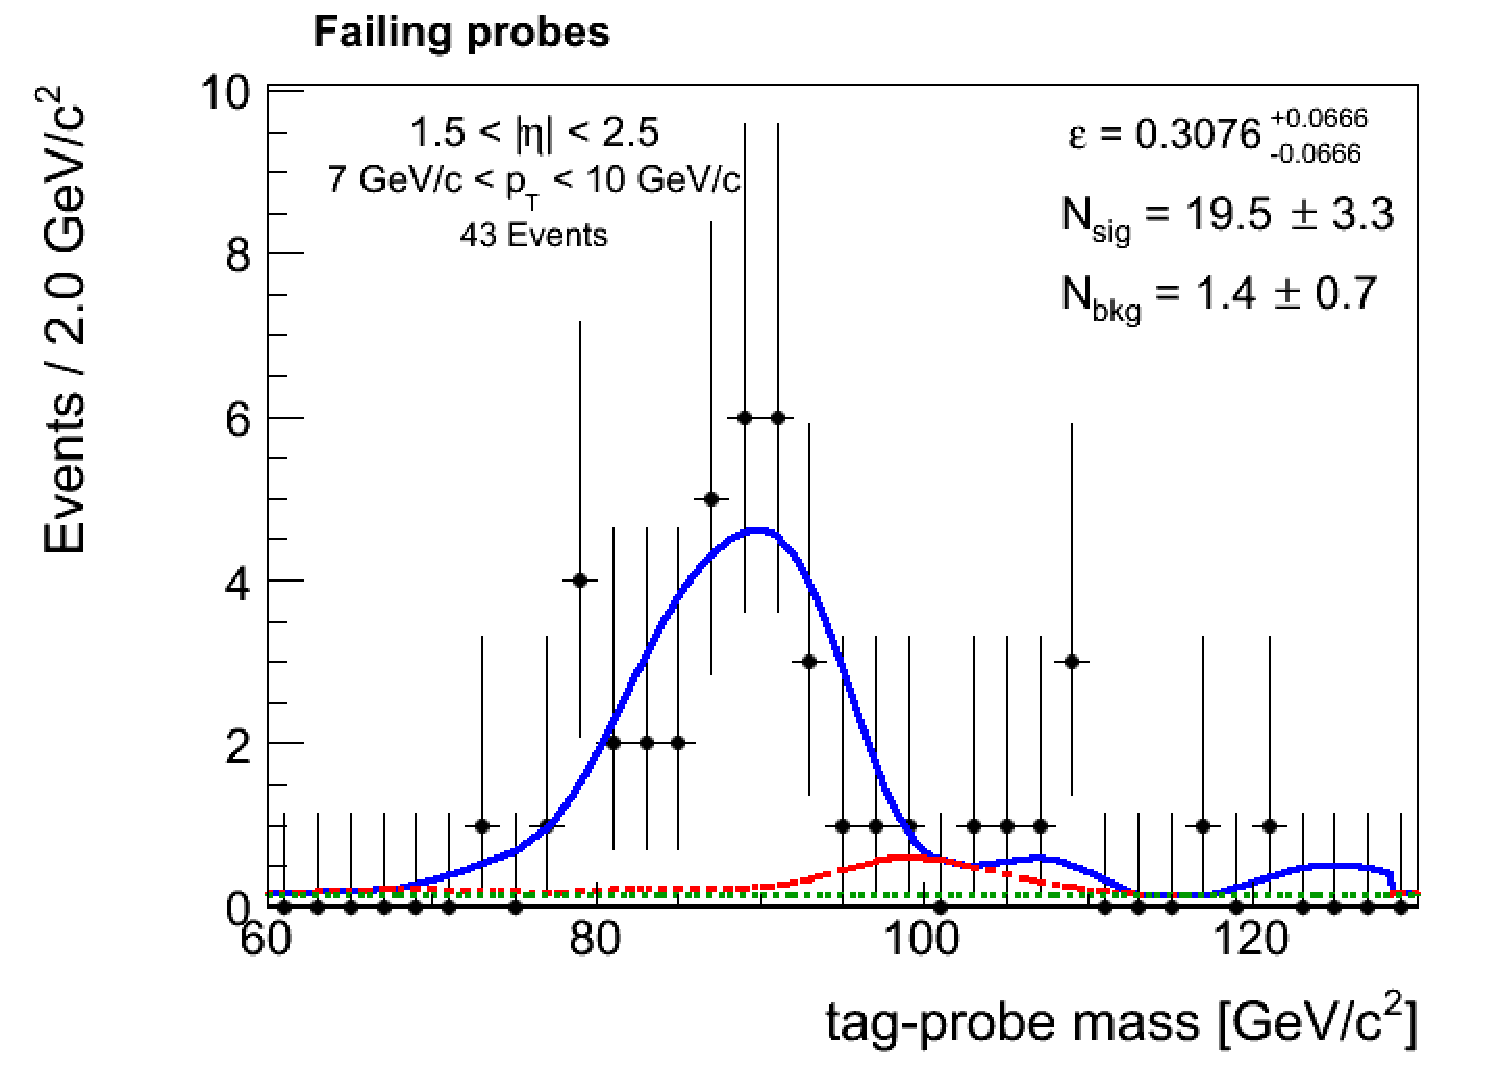
\includegraphics[width=0.48\textwidth]{figures/failetapt_TemplateConvGausPlusExpFit_1.pdf}}
    \caption{Fits to the $m_{ee\gamma}$ distribution are shown for the pass and fail samples for
      electron probes with $p_{T}$ between $7$~\GeV\ and $10$~\GeV.
    }
    \label{fig:MassFits_Pt7To10}
  \end{center}
\end{figure}

\begin{figure}[htb]
  \begin{center}
    \subfigure[Barrel Pass]{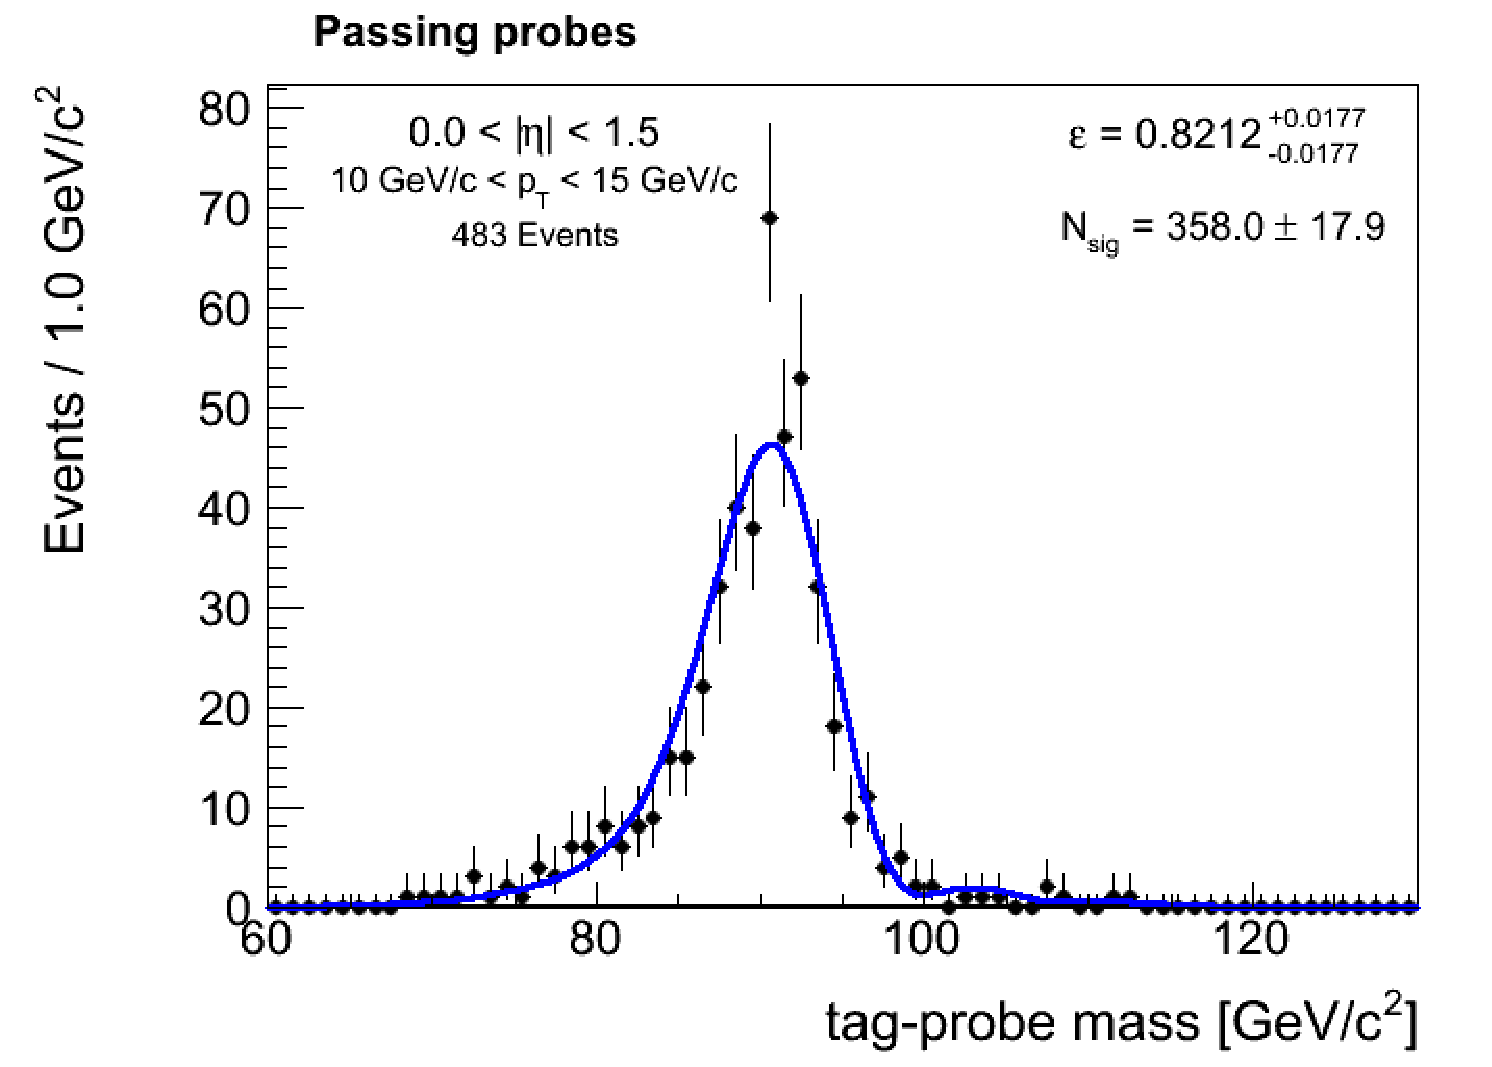
\includegraphics[width=0.48\textwidth]{figures/passetapt_TemplateConvGausPlusExpFit_2.pdf}}
    \subfigure[Barrel Fail]{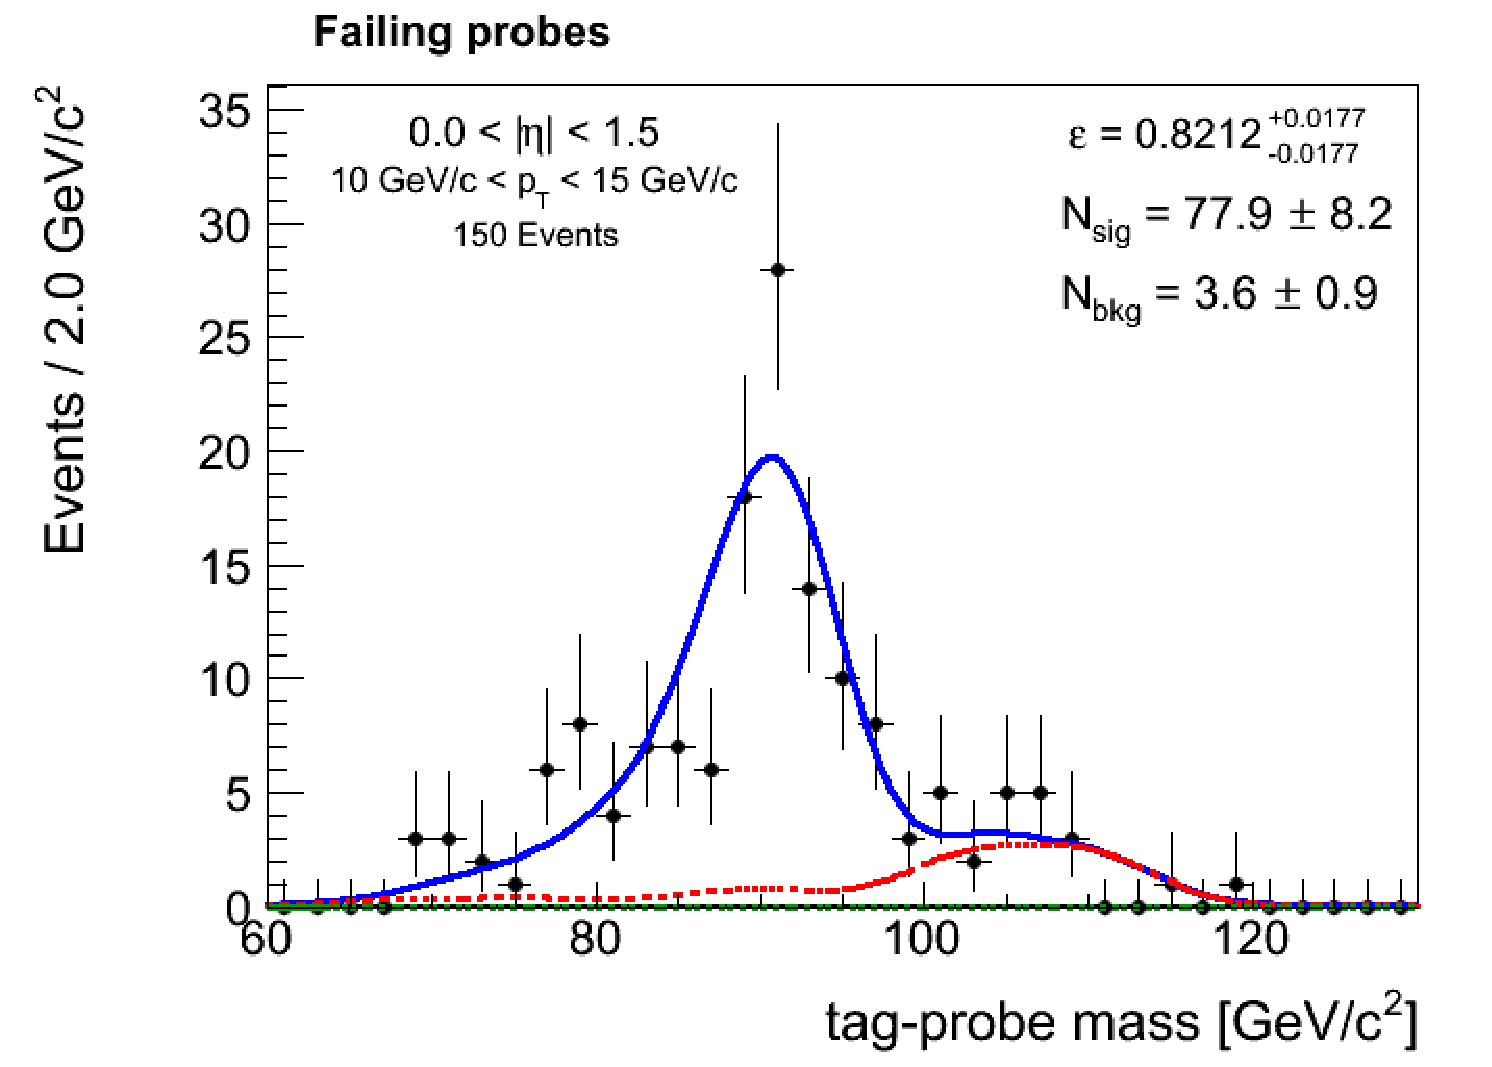
\includegraphics[width=0.48\textwidth]{figures/failetapt_TemplateConvGausPlusExpFit_2.pdf}}
    \subfigure[Endcap Pass]{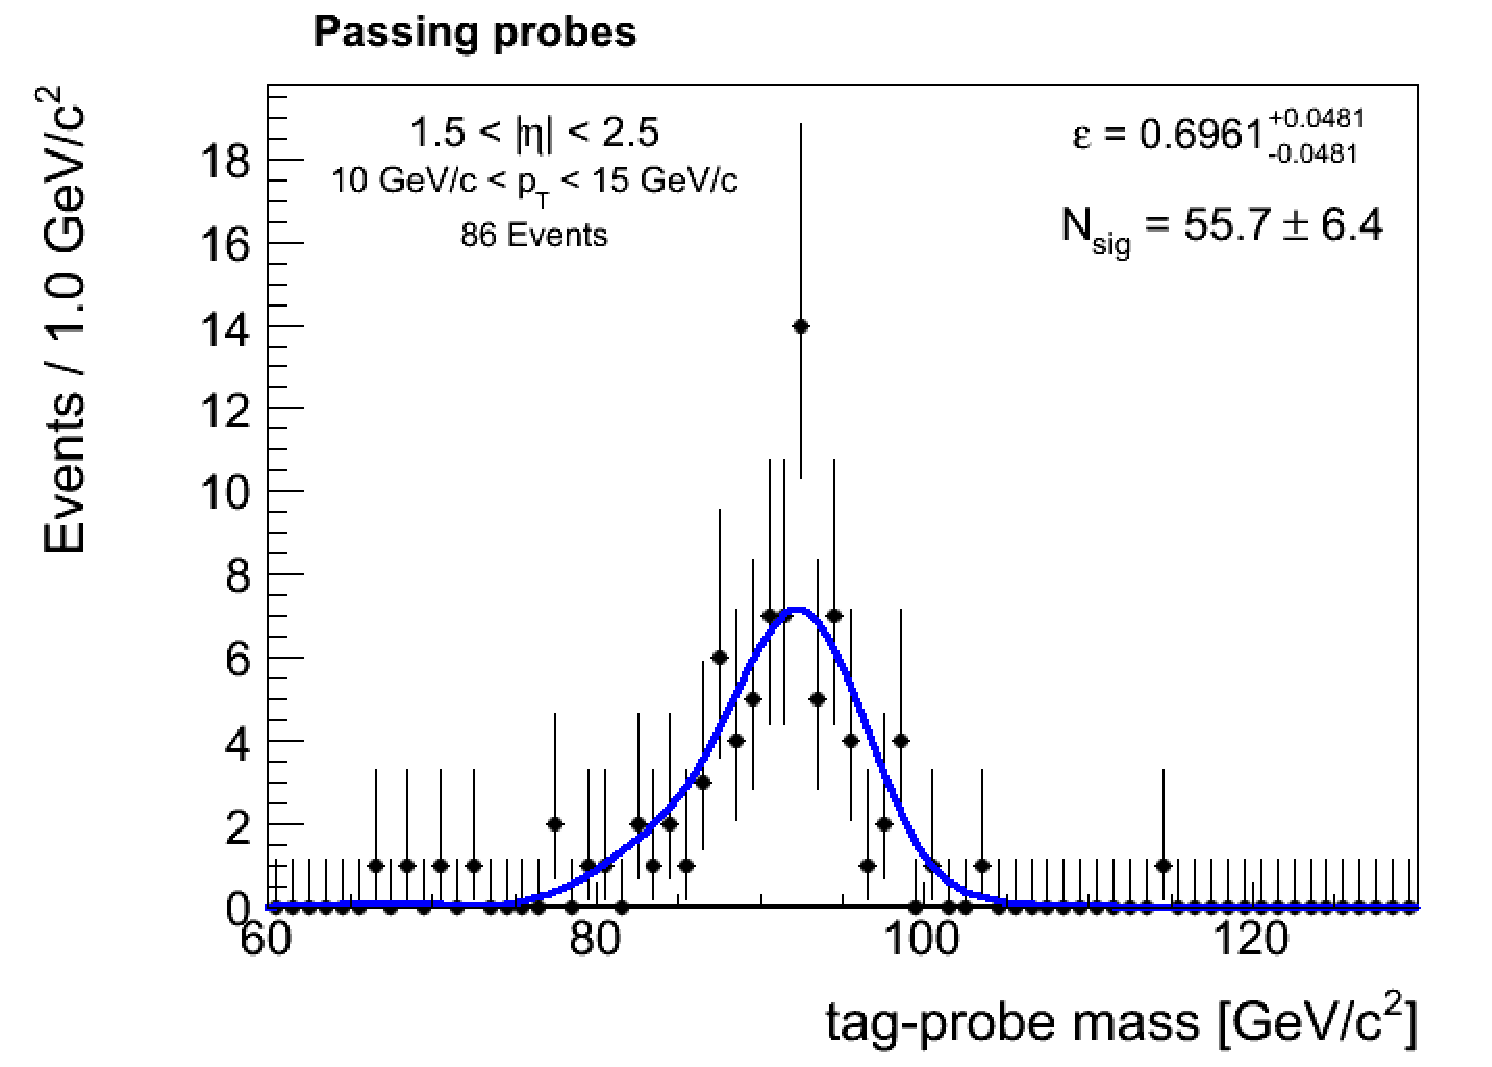
\includegraphics[width=0.48\textwidth]{figures/passetapt_TemplateConvGausPlusExpFit_3.pdf}}
    \subfigure[Endcap Fail]{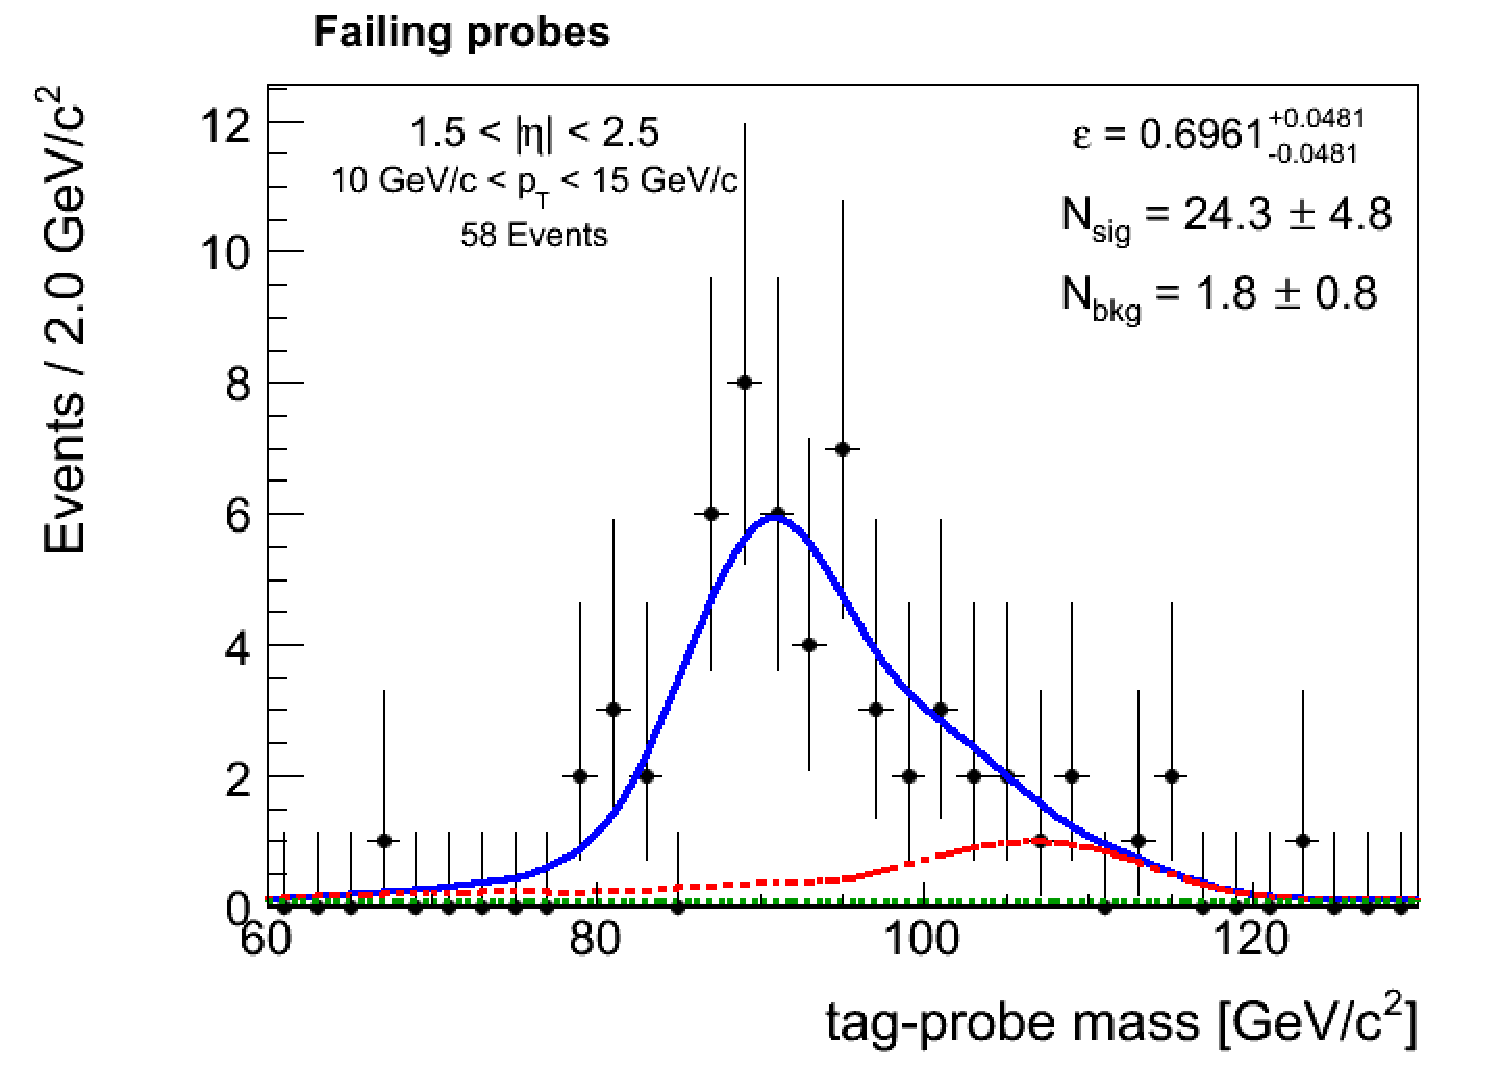
\includegraphics[width=0.48\textwidth]{figures/failetapt_TemplateConvGausPlusExpFit_3.pdf}}
    \caption{Fits to the $m_{ee\gamma}$ distribution are shown for the pass and fail samples for
      electron probes with $p_{T}$ between $10$~\GeV\ and $15$~\GeV.
    }
    \label{fig:MassFits_Pt10To15}
  \end{center}
\end{figure}

\begin{figure}[htb]
  \begin{center}
    \subfigure[Barrel Pass]{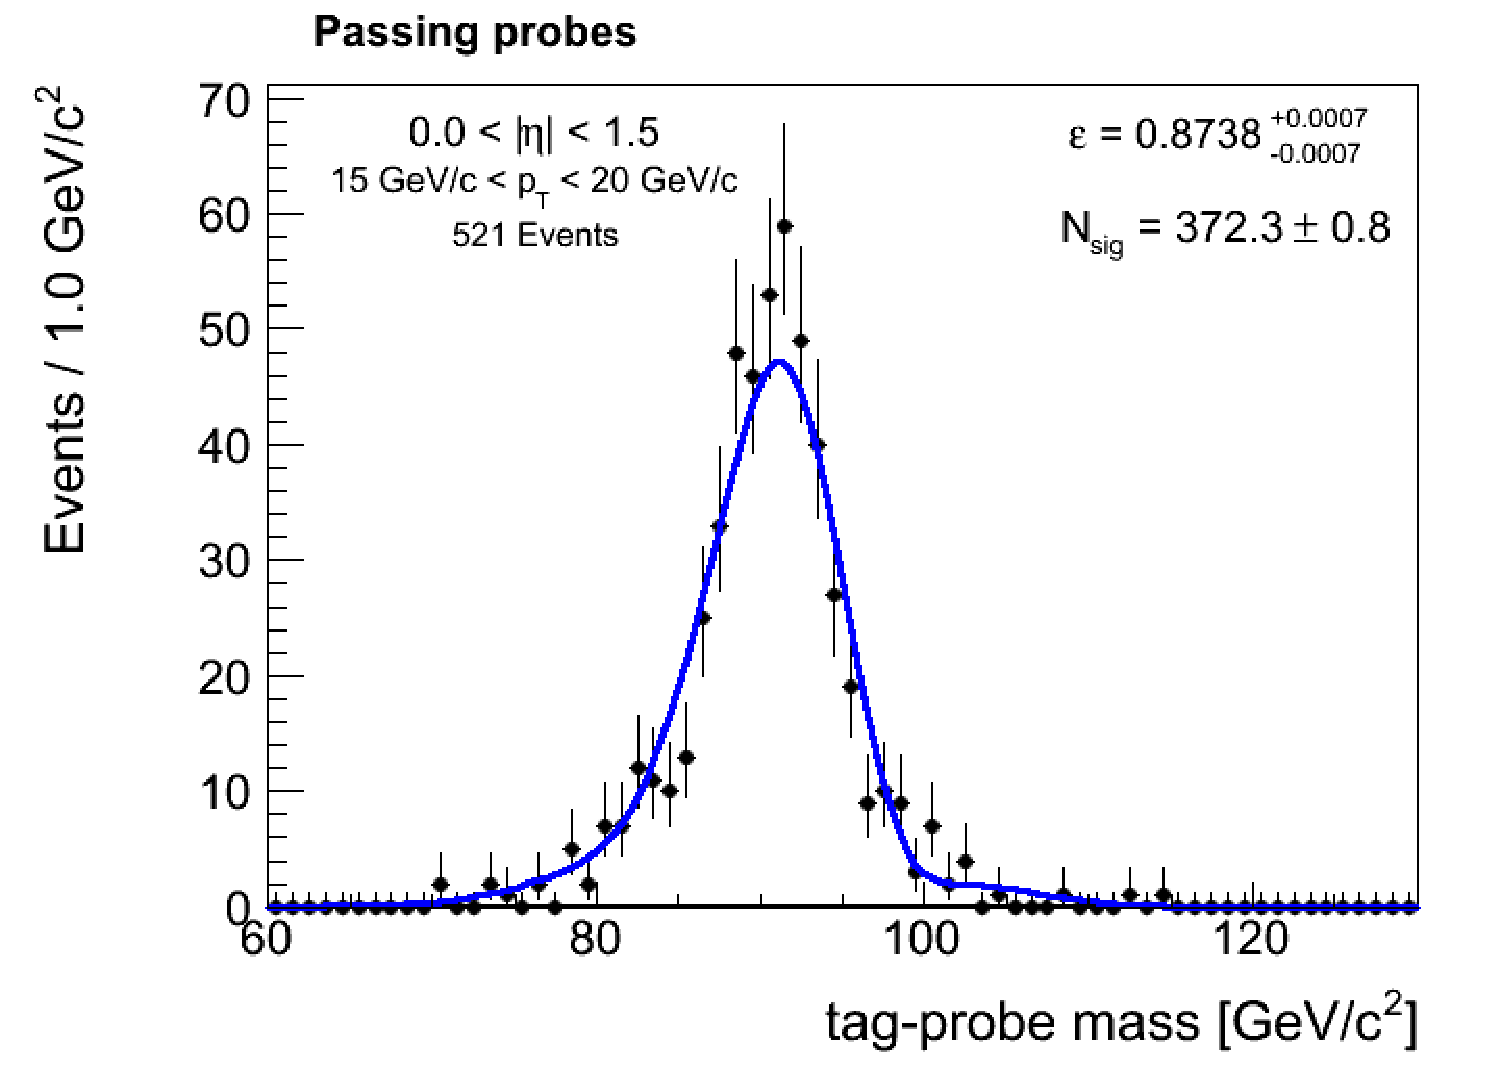
\includegraphics[width=0.48\textwidth]{figures/passetapt_TemplateConvGausPlusExpFit_4.pdf}}
    \subfigure[Barrel Fail]{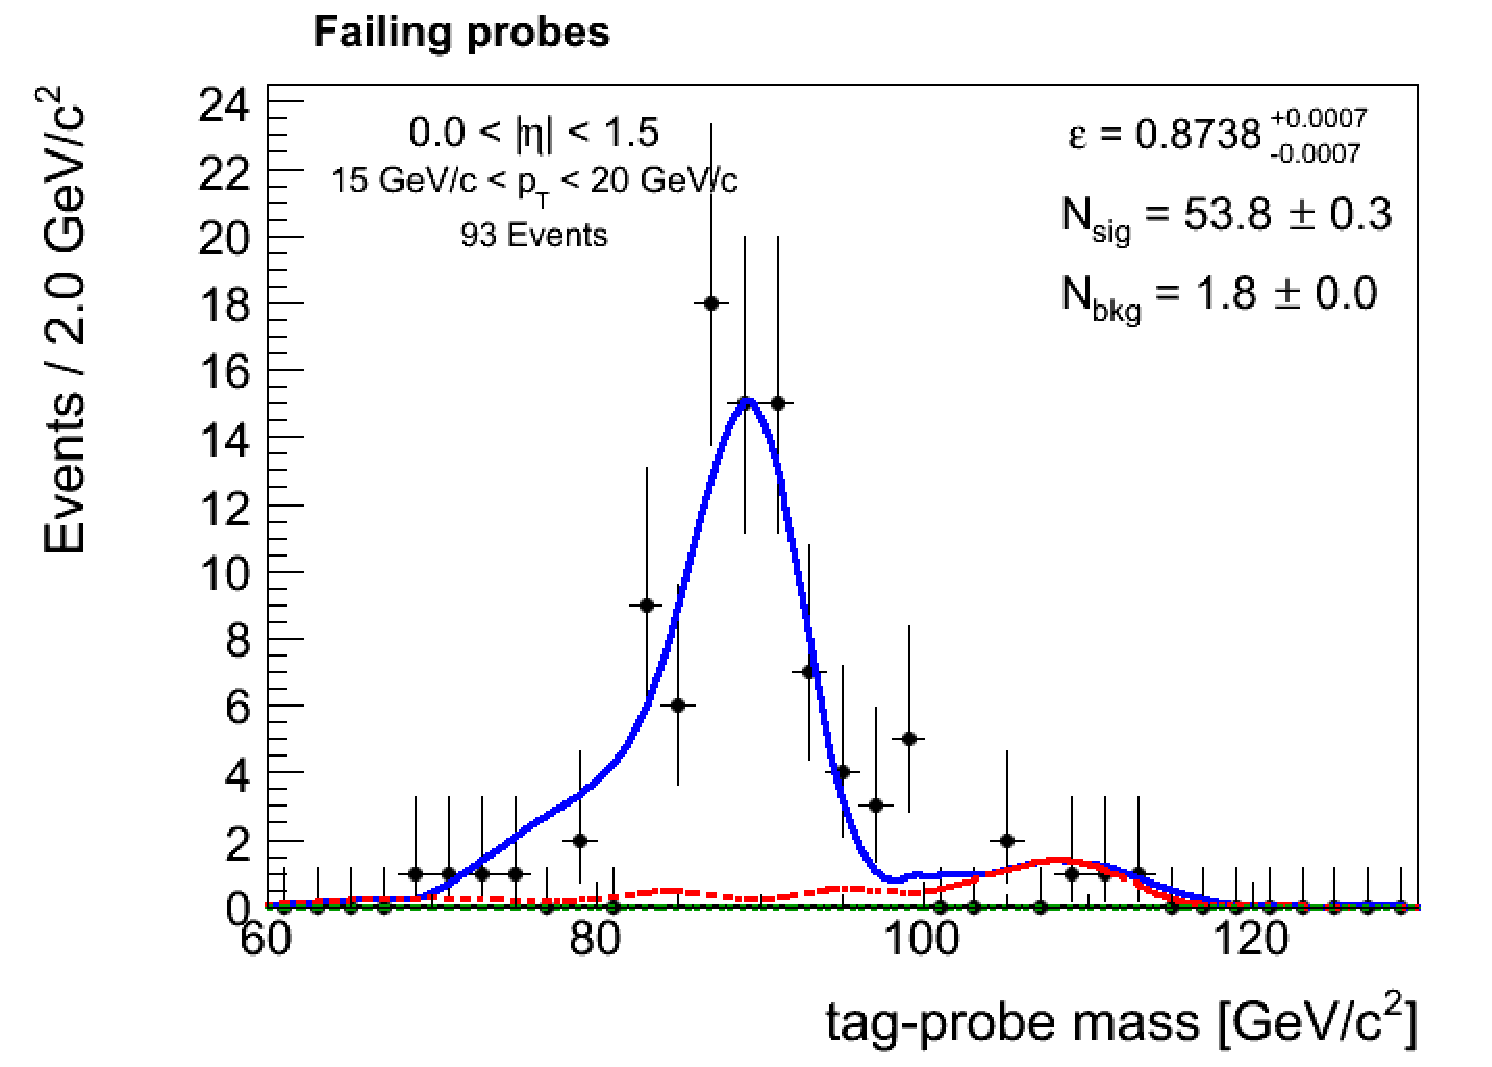
\includegraphics[width=0.48\textwidth]{figures/failetapt_TemplateConvGausPlusExpFit_4.pdf}}
    \subfigure[Endcap Pass]{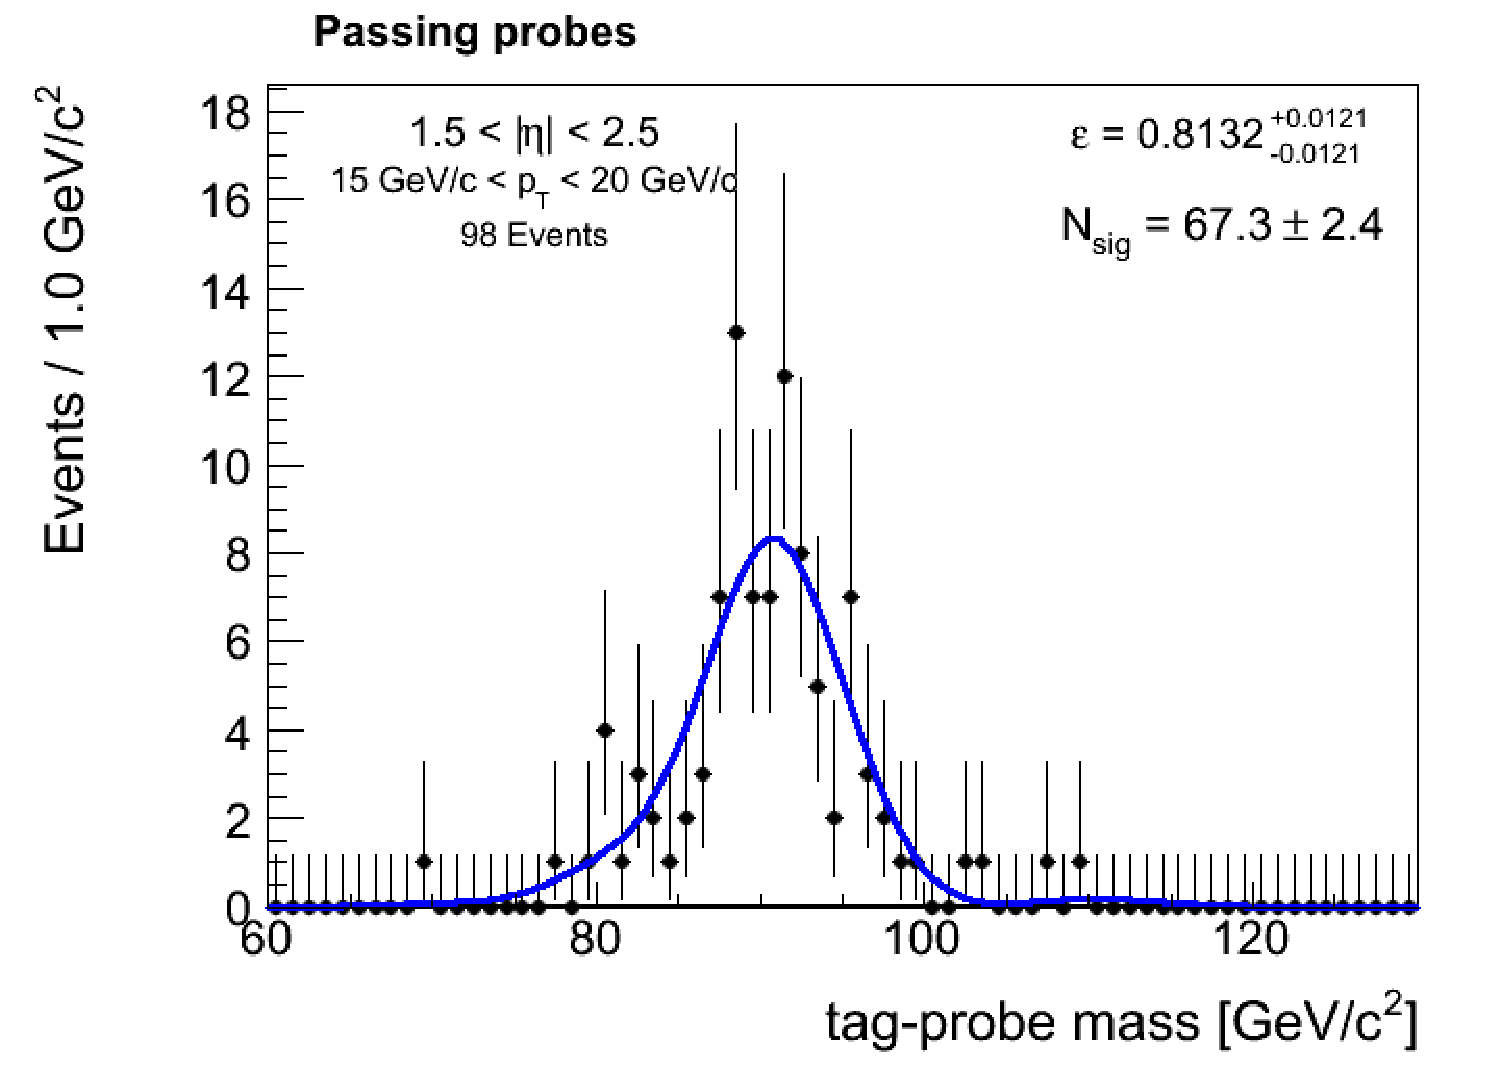
\includegraphics[width=0.48\textwidth]{figures/passetapt_TemplateConvGausPlusExpFit_5.pdf}}
    \subfigure[Endcap Fail]{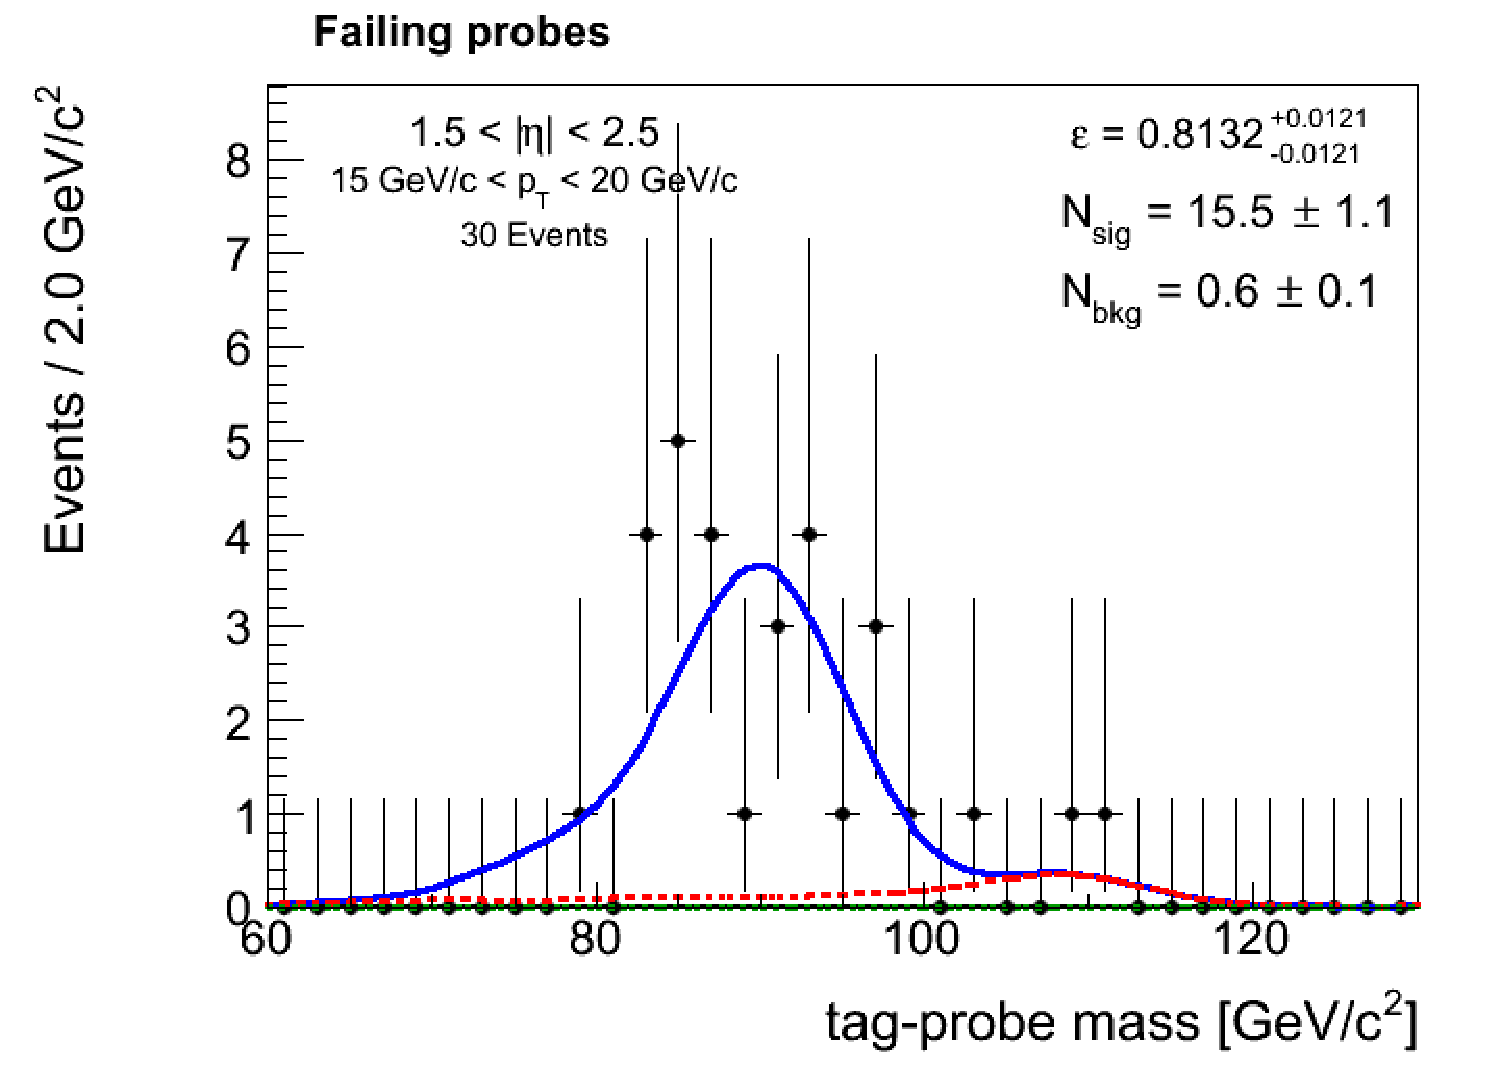
\includegraphics[width=0.48\textwidth]{figures/failetapt_TemplateConvGausPlusExpFit_5.pdf}}
    \caption{Fits to the $m_{ee\gamma}$ distribution are shown for the pass and fail samples for
      electron probes with $p_{T}$ between $15$~\GeV\ and $20$~\GeV.
    }
    \label{fig:MassFits_Pt15To20}
  \end{center}
\end{figure}

 \begin{table}[!ht]
 \begin{center} 
 \begin{tabular}{|c|c|c|c|}
 \hline
 $p_{T}$ / $\eta$ bin    &  Monte Carlo Efficiency    &  Data Efficiency   &  MC to Data Scale Factor \\   \hline           
$  7.0 < p_{T} \le  10.0$ , $  0.0  \le |\eta| <   1.5$   &       0.6907 +/- 0.0274   &       0.5518 +/- 0.0429   &       0.7989 +/- 0.0697   \\   
\hline
$  7.0 < p_{T} \le  10.0$ , $  1.5  \le |\eta| <   2.5$   &       0.4819 +/- 0.0607   &       0.3076 +/- 0.0666   &       0.6382 +/- 0.1598   \\   
\hline
$ 10.0 < p_{T} \le  15.0$ , $  0.0  \le |\eta| <   1.5$   &       0.8330 +/- 0.0130   &       0.8212 +/- 0.0177   &       0.9859 +/- 0.0262   \\   
\hline
$ 10.0 < p_{T} \le  15.0$ , $  1.5  \le |\eta| <   2.5$   &       0.6833 +/- 0.0344   &       0.6961 +/- 0.0481   &       1.0188 +/- 0.0870   \\   
\hline
$ 15.0 < p_{T} \le  20.0$ , $  0.0  \le |\eta| <   1.5$   &       0.8875 +/- 0.0107   &       0.8738 +/- 0.0007   &       0.9845 +/- 0.0119   \\   
\hline
$ 15.0 < p_{T} \le  20.0$ , $  1.5  \le |\eta| <   2.5$   &       0.8411 +/- 0.0261   &       0.8132 +/- 0.0121   &       0.9668 +/- 0.0333   \\   
\hline
$ 20.0 < p_{T} $ , $  0.0  \le |\eta| <   1.5$   &       0.9246 +/- 0.0058   &       0.9209 +/- 0.0076   &       0.9959 +/- 0.0103   \\   
\hline
$ 20.0 < p_{T} $ , $  1.5  \le |\eta| <   2.5$   &       0.9035 +/- 0.0148   &       0.8745 +/- 0.0206   &       0.9679 +/- 0.0277   \\   
\hline
\end{tabular}
\caption{The efficiencies for the electron selection used in the \HiggsToZZ\ analysis for ICHEP 2012
measured from the Monte Carlo simulation and the data, and the Monte Carlo
to data scale factors are shown for different bins of $p_{T}$ and $\eta$. }
\label{tab:Efficiency_HZZICHEP2012WP}
\end{center}
\end{table}

To perform further cross checks of these efficiency scale factors, we measure the efficiency of the isolation
requirement only. These efficiencies are summarized in Table \ref{tab:Efficiency_HZZICHEP2012Iso}. In this case,
we observe that all scale factors are statistically consistent with $1.0$, and conclude that the significant scale 
factor correction is not a result of the isolation. 

 \begin{table}[!ht]
 \begin{center} 
 \begin{tabular}{|c|c|c|c|}
 \hline
 $p_{T}$ / $\eta$ bin    &  Monte Carlo Efficiency    &  Data Efficiency   &  MC to Data Scale Factor \\   \hline           
$  7.0 < p_{T} \le  10.0$ , $  0.0  \le |\eta| <   1.5$   &       0.8232 +/- 0.0224   &       0.7699 +/- 0.0484   &       0.9352 +/- 0.0640   \\   
\hline
$  7.0 < p_{T} \le  10.0$ , $  1.5  \le |\eta| <   2.5$   &       0.8105 +/- 0.0490   &       0.8244 +/- 0.0586   &       1.0171 +/- 0.0949   \\   
\hline
$ 10.0 < p_{T} \le  15.0$ , $  0.0  \le |\eta| <   1.5$   &       0.8866 +/- 0.0108   &       0.8981 +/- 0.0158   &       1.0130 +/- 0.0217   \\   
\hline
$ 10.0 < p_{T} \le  15.0$ , $  1.5  \le |\eta| <   2.5$   &       0.8843 +/- 0.0244   &       0.8747 +/- 0.0375   &       0.9891 +/- 0.0504   \\   
\hline
$ 15.0 < p_{T} \le  20.0$ , $  0.0  \le |\eta| <   1.5$   &       0.9209 +/- 0.0089   &       0.9096 +/- 0.0125   &       0.9877 +/- 0.0166   \\   
\hline
$ 15.0 < p_{T} \le  20.0$ , $  1.5  \le |\eta| <   2.5$   &       0.9253 +/- 0.0192   &       0.9852 +/- 0.0079   &       1.0648 +/- 0.0236   \\   
\hline
$ 20.0 < p_{T} $ , $  0.0  \le |\eta| <   1.5$   &       0.9529 +/- 0.0037   &       0.9508 +/- 0.0055   &       0.9978 +/- 0.0069   \\   
\hline
$ 20.0 < p_{T} $ , $  1.5  \le |\eta| <   2.5$   &       0.9695 +/- 0.0074   &       0.9941 +/- 0.0088   &       1.0254 +/- 0.0120   \\   
\hline
\end{tabular}
\caption{The efficiencies for the electron isolation requirement measured from the Monte Carlo simulation and the data, and the Monte Carlo
to data scale factors are shown for different bins of $p_{T}$ and $\eta$. }
\label{tab:Efficiency_HZZICHEP2012Iso}
\end{center}
\end{table}

Next we measure the efficiency of the BDT electron identification and impact parameter significance requirements 
given that the electron already passed the isolation requirement. This isolation requirement reduces 
the background to a negligible level, allowing the efficiency
to be measured simply by counting passing and failing probes. The resulting efficiencies and scale factors are shown in
Table \ref{tab:Efficiency_HZZICHEP2012IDGivenIso}. We observe that the scale factors for the lowest $p_{T}$ bins
are statistically consistent with the scale factors obtained for the full selection efficiency. This confirms that the
disagreement between data and Monte Carlo is originating from the BDT electron identification and impact parameter significance 
requirements. As a final cross check we measure the efficiency of the isolation requirement given that the 
electron already passed the identification and impact parameter significance requirements. These efficiencies are summarized in 
Table \ref{tab:Efficiency_HZZICHEP2012IsoGivenID} and demonstrate again that the isolation efficiency agrees between
data and Monte Carlo simulation. 


 \begin{table}[!ht]
 \begin{center} 
 \begin{tabular}{|c|c|c|c|}
 \hline
 $p_{T}$ / $\eta$ bin    &  Monte Carlo Efficiency    &  Data Efficiency   &  MC to Data Scale Factor \\   \hline           
$  7.0 < p_{T} \le  10.0$ , $  0.0  \le |\eta| <   1.5$   &       0.8423 +/- 0.0240   &       0.7185 +/- 0.0349   &       0.8531 +/- 0.0480   \\   
\hline
$  7.0 < p_{T} \le  10.0$ , $  1.5  \le |\eta| <   2.5$   &       0.6364 +/- 0.0629   &       0.4103 +/- 0.0762   &       0.6447 +/- 0.1338   \\   
\hline
$ 10.0 < p_{T} \le  15.0$ , $  0.0  \le |\eta| <   1.5$   &       0.9383 +/- 0.0091   &       0.9406 +/- 0.0100   &       1.0025 +/- 0.0144   \\   
\hline
$ 10.0 < p_{T} \le  15.0$ , $  1.5  \le |\eta| <   2.5$   &       0.7710 +/- 0.0324   &       0.7453 +/- 0.0385   &       0.9666 +/- 0.0643   \\   
\hline
$ 15.0 < p_{T} \le  20.0$ , $  0.0  \le |\eta| <   1.5$   &       0.9575 +/- 0.0072   &       0.9522 +/- 0.0090   &       0.9944 +/- 0.0121   \\   
\hline
$ 15.0 < p_{T} \le  20.0$ , $  1.5  \le |\eta| <   2.5$   &       0.8962 +/- 0.0225   &       0.8083 +/- 0.0326   &       0.9020 +/- 0.0427   \\   
\hline
$ 20.0 < p_{T} $ , $  0.0  \le |\eta| <   1.5$   &       0.9768 +/- 0.0028   &       0.9749 +/- 0.0033   &       0.9980 +/- 0.0044   \\   
\hline
$ 20.0 < p_{T} $ , $  1.5  \le |\eta| <   2.5$   &       0.9476 +/- 0.0094   &       0.9115 +/- 0.0138   &       0.9620 +/- 0.0174   \\   
\hline
\end{tabular}
\caption{The efficiencies for the electron identification requirement given that the electron passed
  the isolation requirement measured from the Monte Carlo simulation and the data, and the Monte Carlo
to data scale factors are shown for different bins of $p_{T}$ and $\eta$. }
\label{tab:Efficiency_HZZICHEP2012IDGivenIso}
\end{center}
\end{table}

 \begin{table}[!ht]
 \begin{center} 
 \begin{tabular}{|c|c|c|c|}
 \hline
 $p_{T}$ / $\eta$ bin    &  Monte Carlo Efficiency    &  Data Efficiency   &  MC to Data Scale Factor \\   \hline           
$  7.0 < p_{T} \le  10.0$ , $  0.0  \le |\eta| <   1.5$   &       0.8339 +/- 0.0243   &       0.7760 +/- 0.0365   &       0.9306 +/- 0.0515   \\   
\hline
$  7.0 < p_{T} \le  10.0$ , $  1.5  \le |\eta| <   2.5$   &       0.8167 +/- 0.0640   &       0.8421 +/- 0.0920   &       1.0311 +/- 0.1386   \\   
\hline
$ 10.0 < p_{T} \le  15.0$ , $  0.0  \le |\eta| <   1.5$   &       0.8939 +/- 0.0109   &       0.9035 +/- 0.0117   &       1.0108 +/- 0.0180   \\   
\hline
$ 10.0 < p_{T} \le  15.0$ , $  1.5  \le |\eta| <   2.5$   &       0.9066 +/- 0.0268   &       0.9186 +/- 0.0308   &       1.0132 +/- 0.0453   \\   
\hline
$ 15.0 < p_{T} \le  20.0$ , $  0.0  \le |\eta| <   1.5$   &       0.9236 +/- 0.0090   &       0.9317 +/- 0.0097   &       1.0087 +/- 0.0144   \\   
\hline
$ 15.0 < p_{T} \le  20.0$ , $  1.5  \le |\eta| <   2.5$   &       0.9357 +/- 0.0195   &       0.9510 +/- 0.0228   &       1.0163 +/- 0.0323   \\   
\hline
$ 20.0 < p_{T} $ , $  0.0  \le |\eta| <   1.5$   &       0.9542 +/- 0.0037   &       0.9500 +/- 0.0046   &       0.9956 +/- 0.0062   \\   
\hline
$ 20.0 < p_{T} $ , $  1.5  \le |\eta| <   2.5$   &       0.9731 +/- 0.0073   &       0.9913 +/- 0.0056   &       1.0187 +/- 0.0096   \\   
\hline
\end{tabular}
\caption{The efficiencies for the electron isolation requirement given that the electron passed the identification
  requirements measured from the Monte Carlo simulation and the data, and the Monte Carlo
  to data scale factors are shown for different bins of $p_{T}$ and $\eta$. }
\label{tab:Efficiency_HZZICHEP2012IsoGivenID}
\end{center}
\end{table}



\section{Systematic Uncertainties}
The main systematic uncertainty on the efficiency result from the uncertainty on the signal and 
background models induced by potential differences in the energy scale and resolution between
the Monte Carlo simulation and the data. The bulk of this effect is already accounted for 
in the fit where we allow the energy scale and resolution parameters to float unconstrained. 
These nuisances parameters are profiled and the uncertainty intervals obtained from the likelihood
include this systematic uncertainty. 

The remaining dominant uncertainty results from the assumption that this energy scale and resolution
difference are identical for the signal and background. To assess the impact of this systematic uncertainty, 
we throw toy experiments assuming that the energy scale correction for the data and the simulation
differ by $1$~\GeV, $10\%$ of the difference in their respective mass peaks, 
for the signal and the background and perform the fit assuming no such difference. Given the precision
of our energy scale measurements and the proximity of the kinematic regions between the signal and background,
this shift of $10\%$ is a fairly conservative estimate of any potential systematic error. 
The variations of the mass distribution for the models applying these different assumptions are illustrated in 
Fig \ref{fig:SystematicsModels}.



\begin{figure}[htb]
  \begin{center}
    \subfigure[Shift $-1$~$\GeV$]{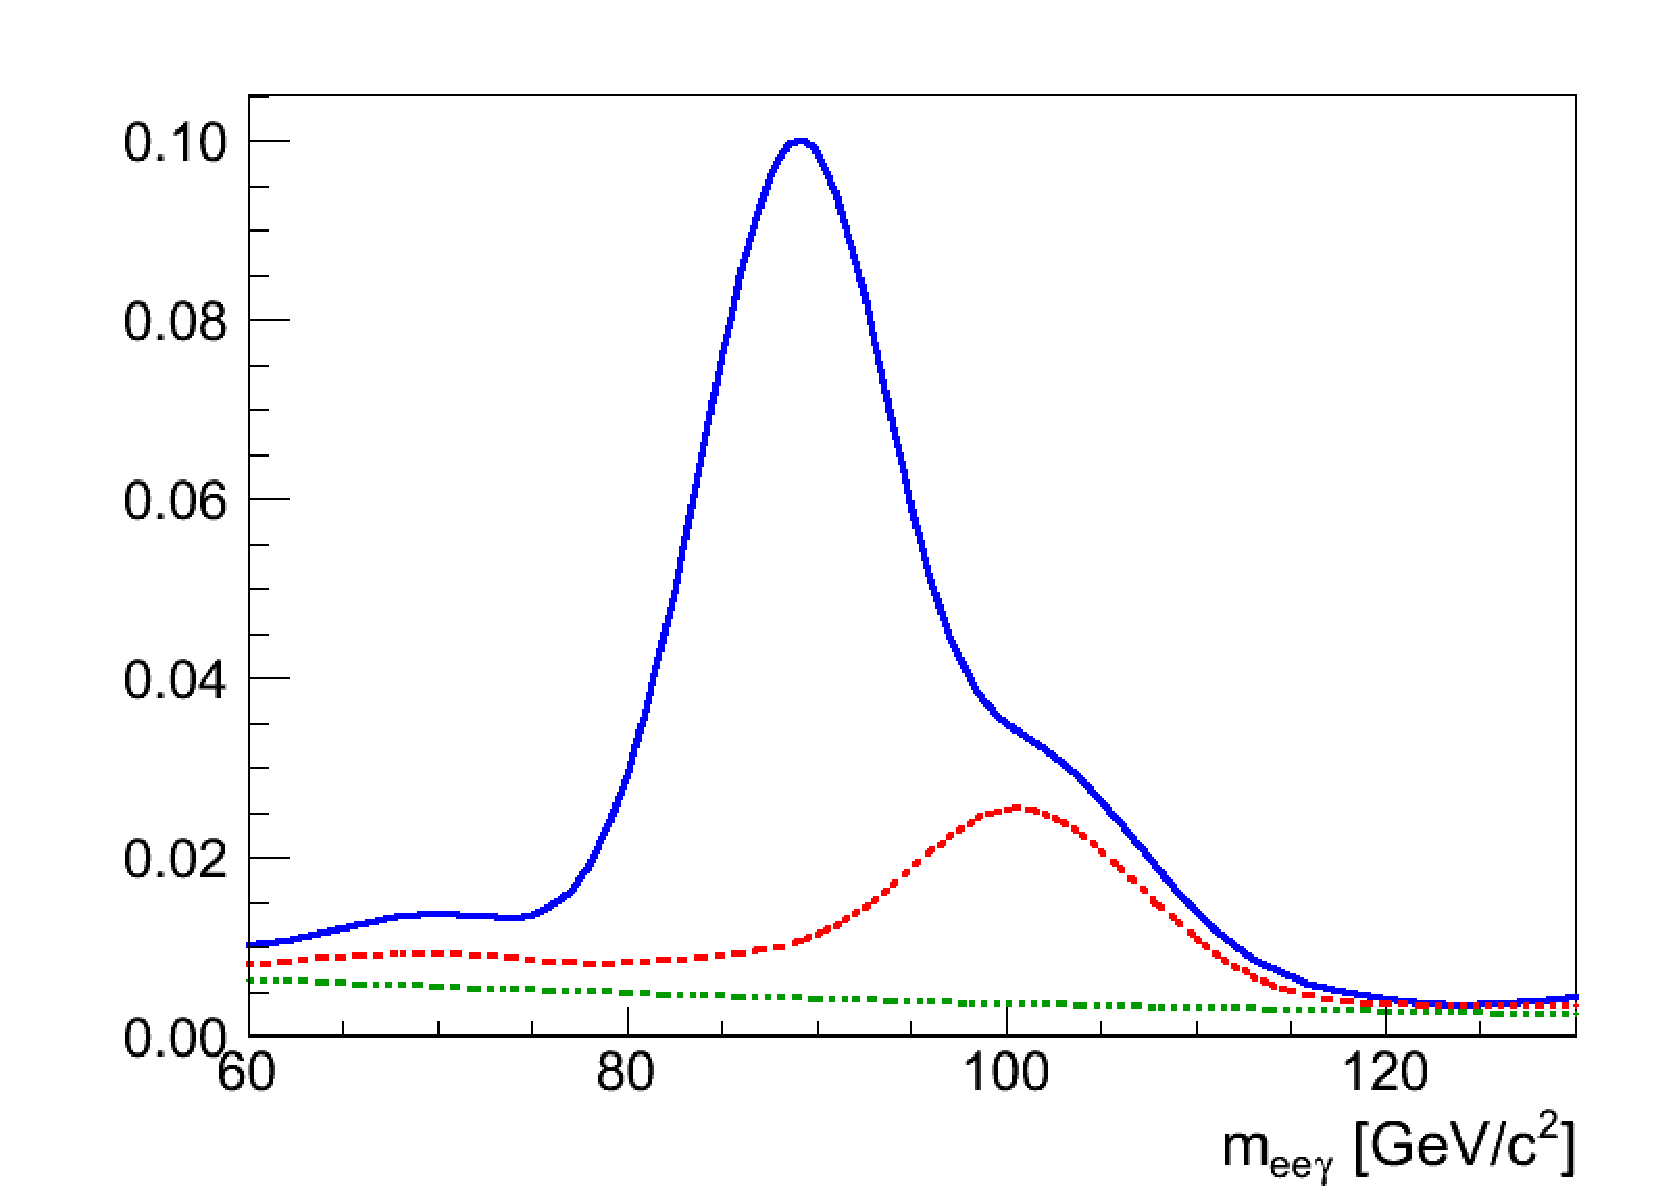
\includegraphics[width=0.32\textwidth]{figures/Model_ShiftMinus1GeV.pdf}}
    \subfigure[Nominal]{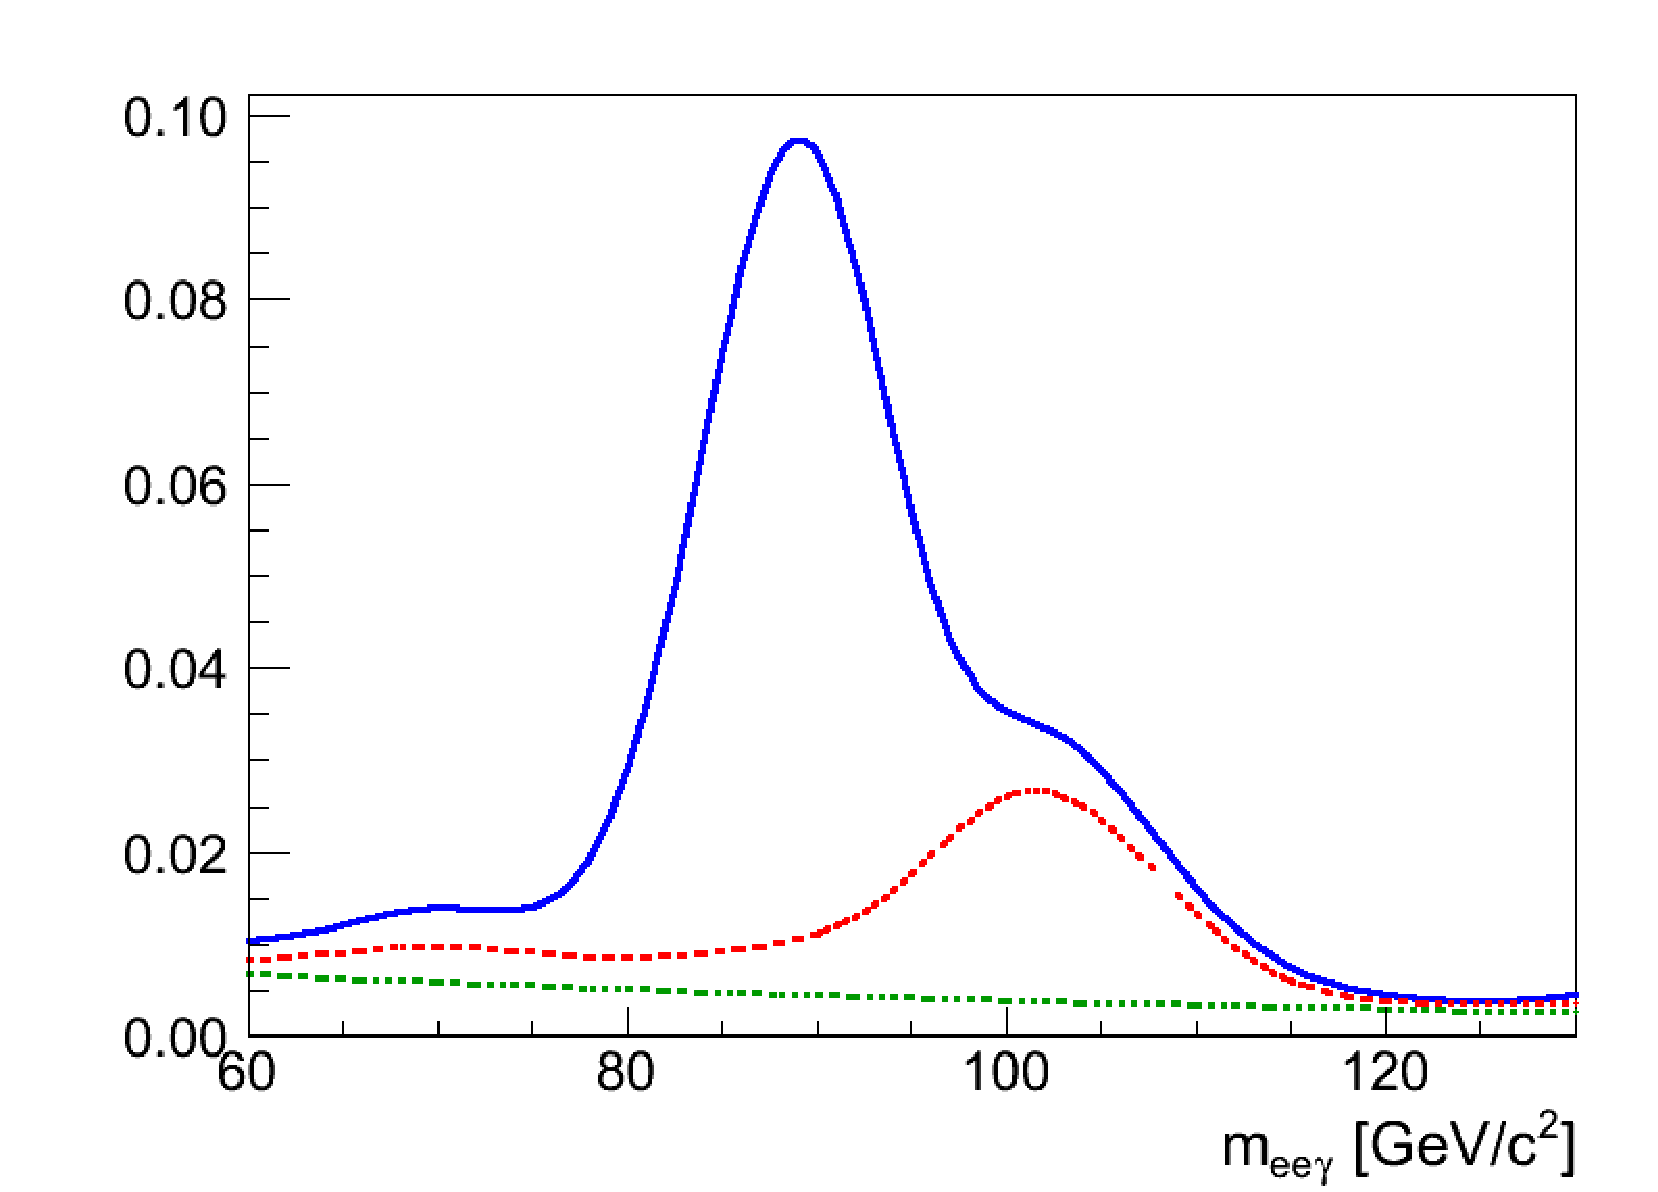
\includegraphics[width=0.32\textwidth]{figures/Model_Nominal.pdf}}
    \subfigure[Shift $+1$~$\GeV$]{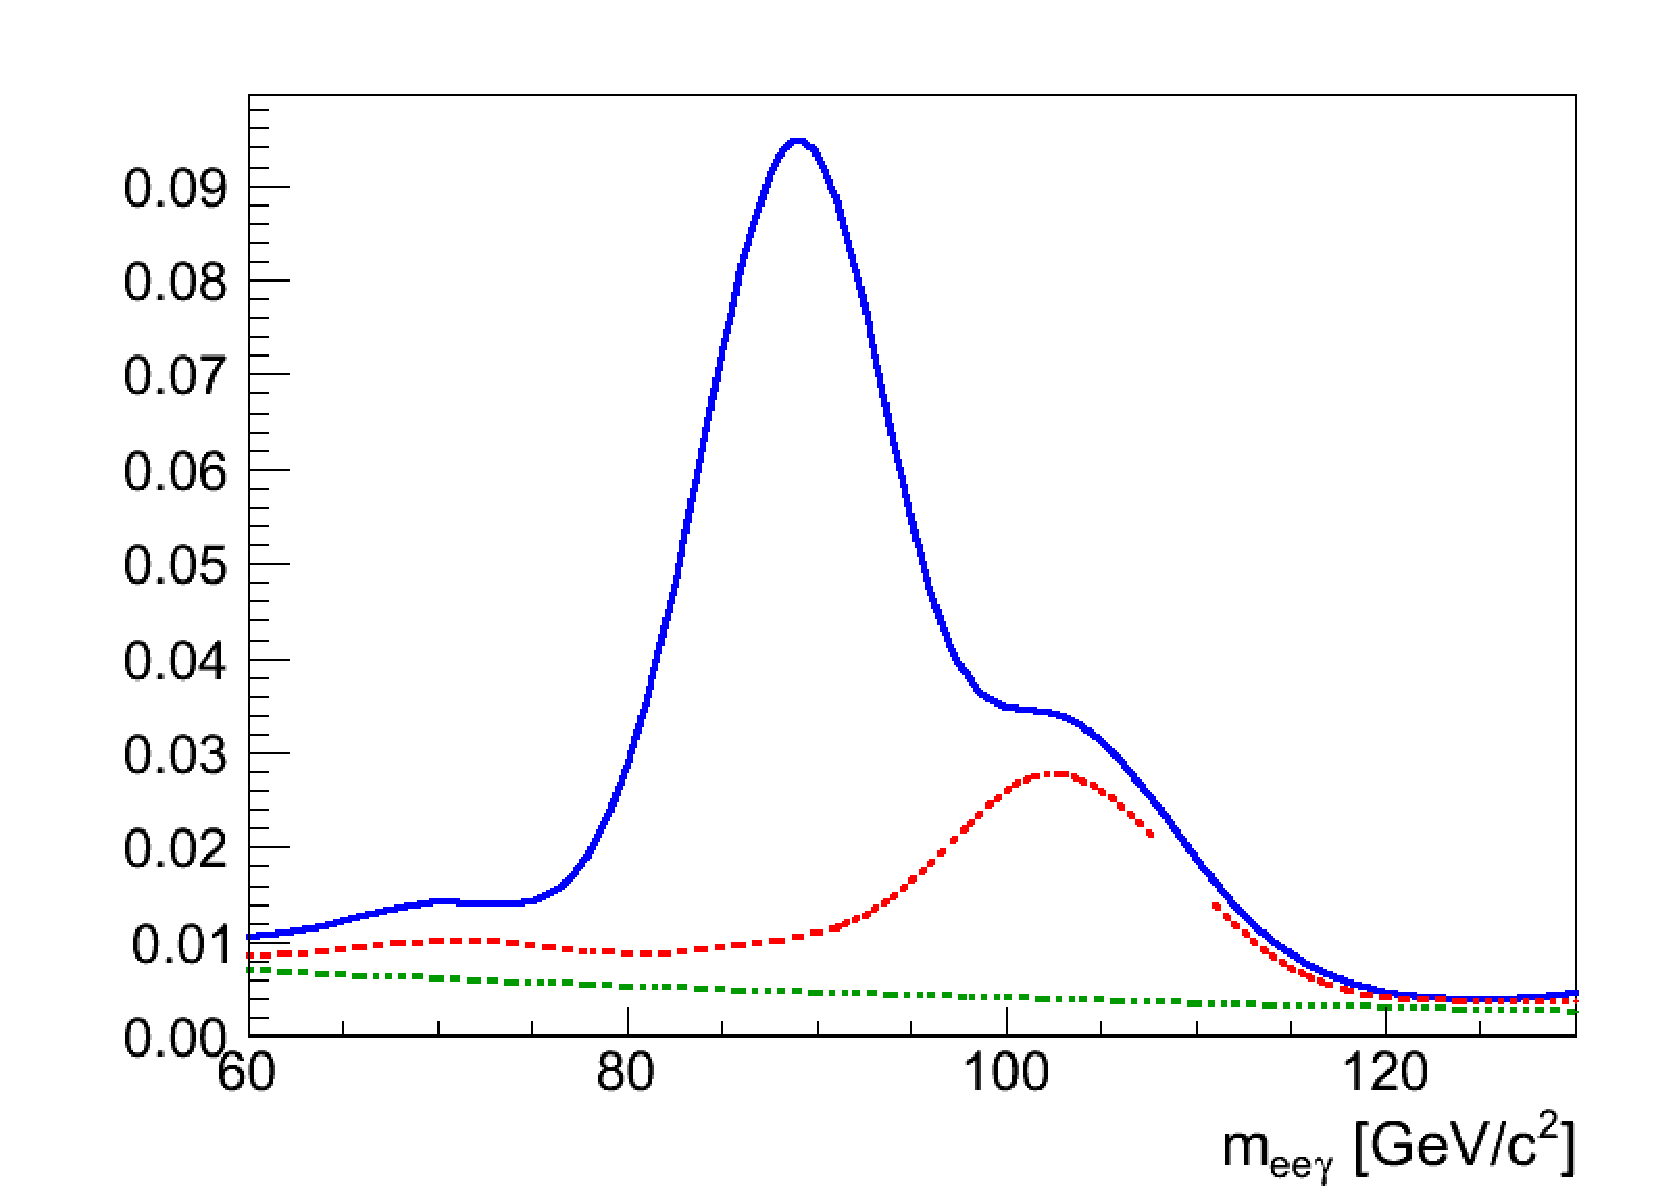
\includegraphics[width=0.32\textwidth]{figures/Model_ShiftPlus1GeV.pdf}}
    \caption{Alternative models of the signal and background for electron probes 
      with $p_{T}$ between $7$~\GeV\ and $10$~\GeV\ which fail the electron selection.
      The green curve represents the exponential component of the background. The red curve is the total background
      comprised of the exponential component and the Drell-Yan fake electron and fake photon component.
      The blue curve is the sum of the signal and the background.
    }
    \label{fig:SystematicsModels}
  \end{center}
\end{figure}



The distributions of the fitted efficiency for the bin with $p_{T}$ between $7$~\GeV\ and $10$~\GeV\ 
and $|eta| < 1.479$ are shown in Fig \ref{fig:EffToys}. The nominal efficiency for this bin is $0.550$. 
The mean efficiency for the set of toys generated with the nominal model is $0.549$, so no 
bias is observed from the fitting procedure. The mean efficiency for the set of toys generated with 
a shift of $+1$~\GeV\ and $-1$~\GeV\ are $0.563\pm0.001$ and $0.542\pm0.001$ respectively. Taking
the largest deviation from the nominal, we estimate a systematic uncertainty of about $2.5\%$
relative to the measured efficiency. This uncertainty is propagated as a systematic uncertainty and added in 
quadrature with the uncertainty obtained from the fit. 


\begin{figure}[htb]
  \begin{center}
    \subfigure[Shift $-1$~$\GeV$]{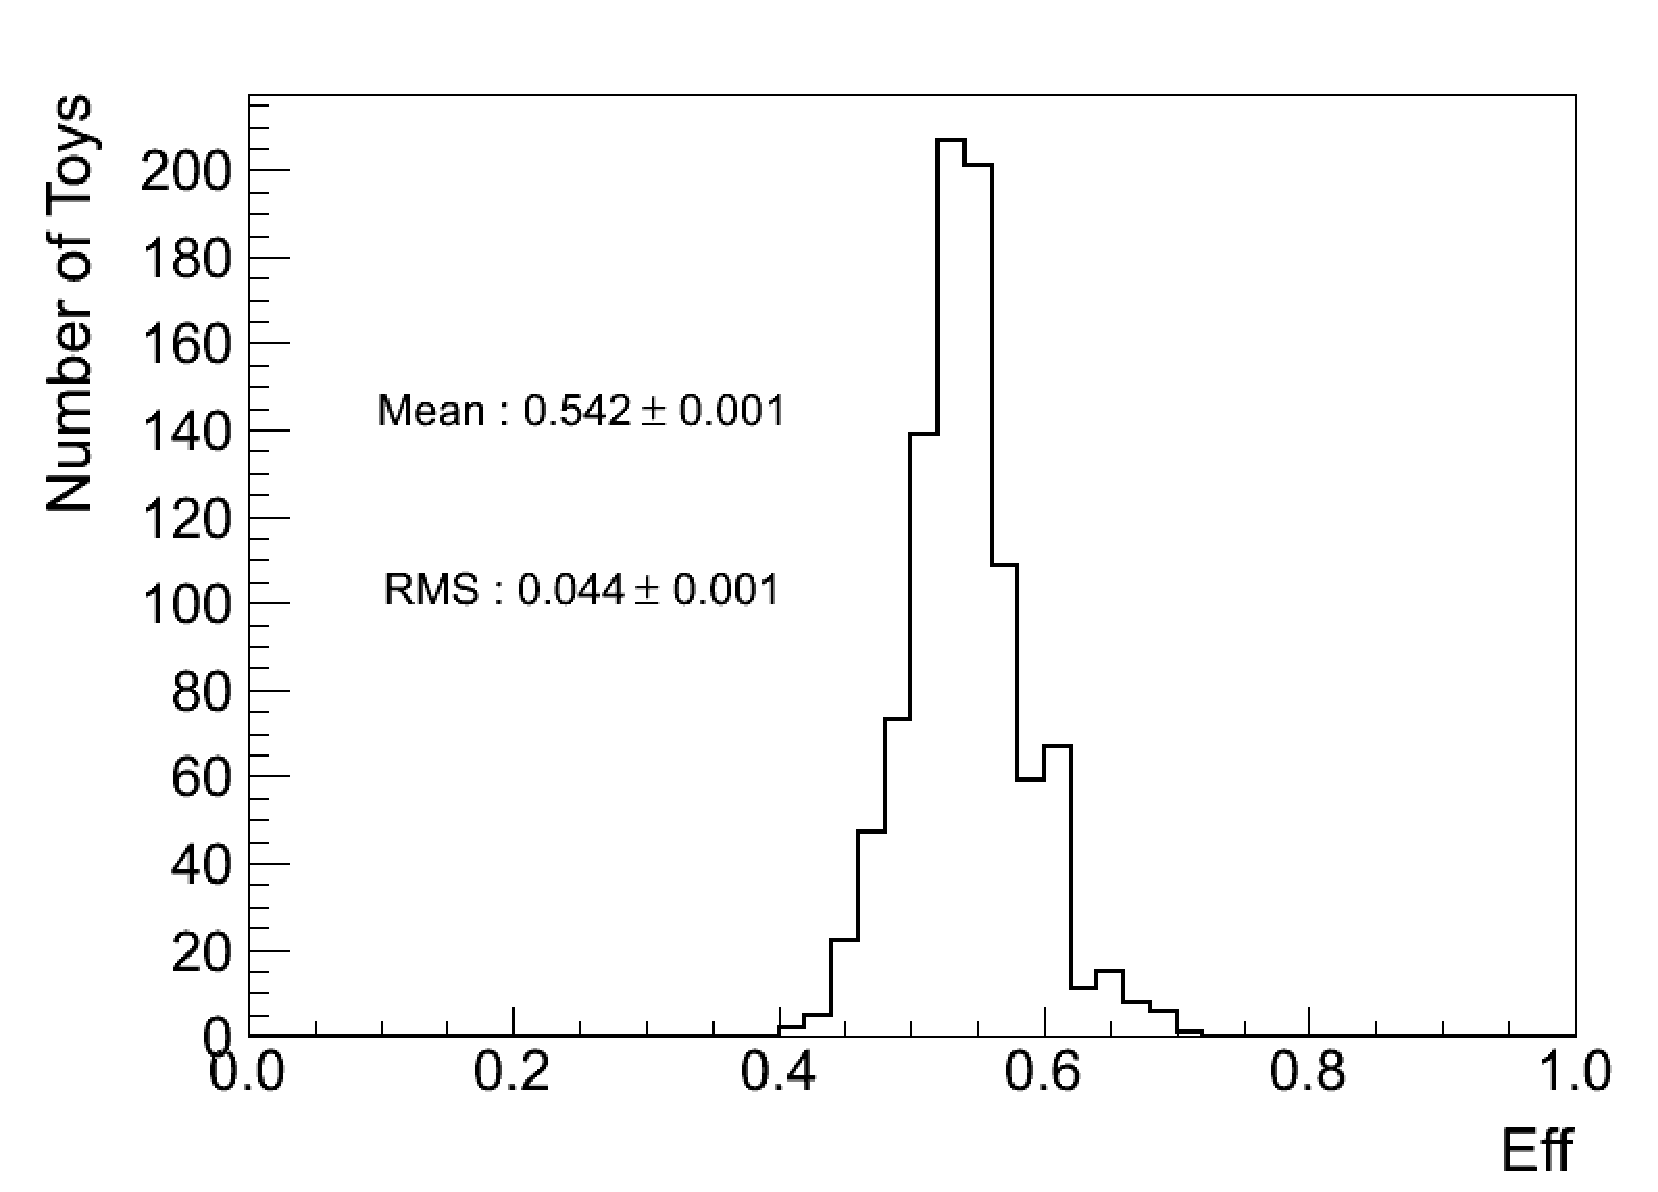
\includegraphics[width=0.48\textwidth]{figures/Eff_ShiftMinus1GeV.pdf}}
    \subfigure[Nominal]{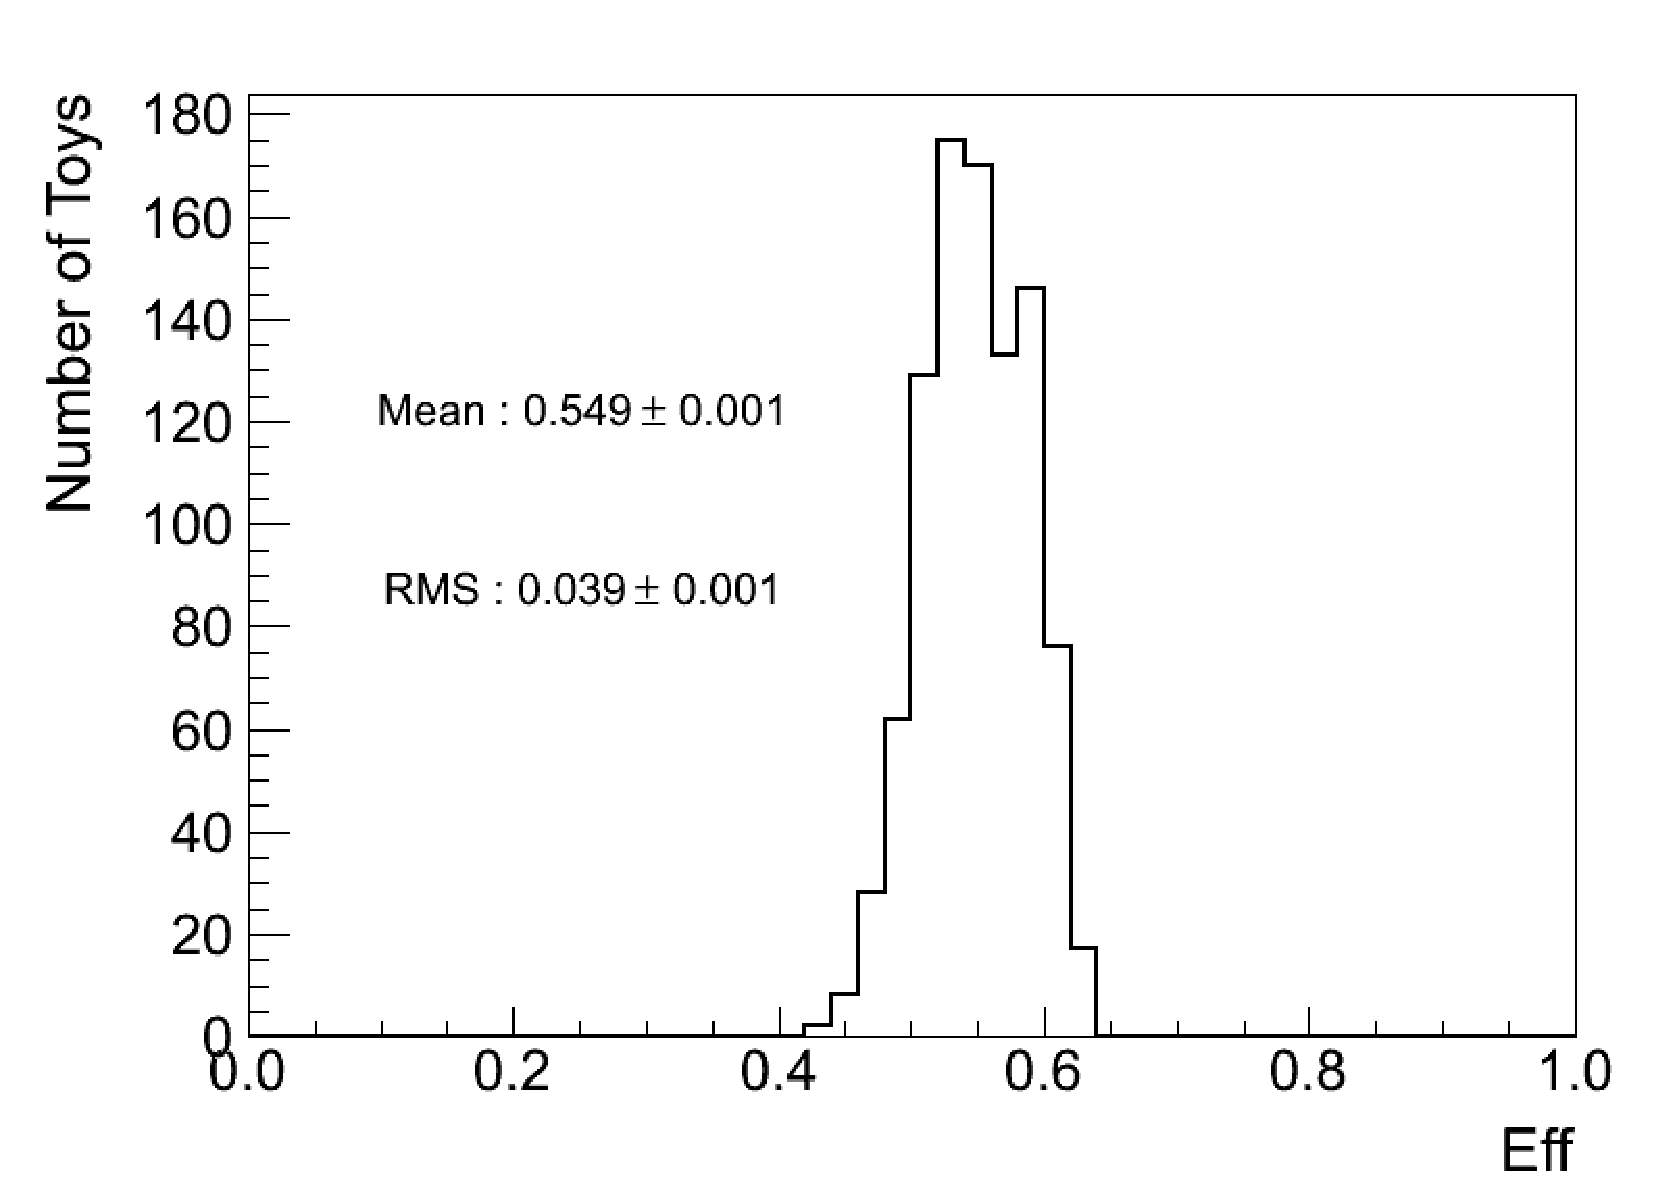
\includegraphics[width=0.48\textwidth]{figures/Eff_Nominal.pdf}}
    \subfigure[Shift $+1$~$\GeV$]{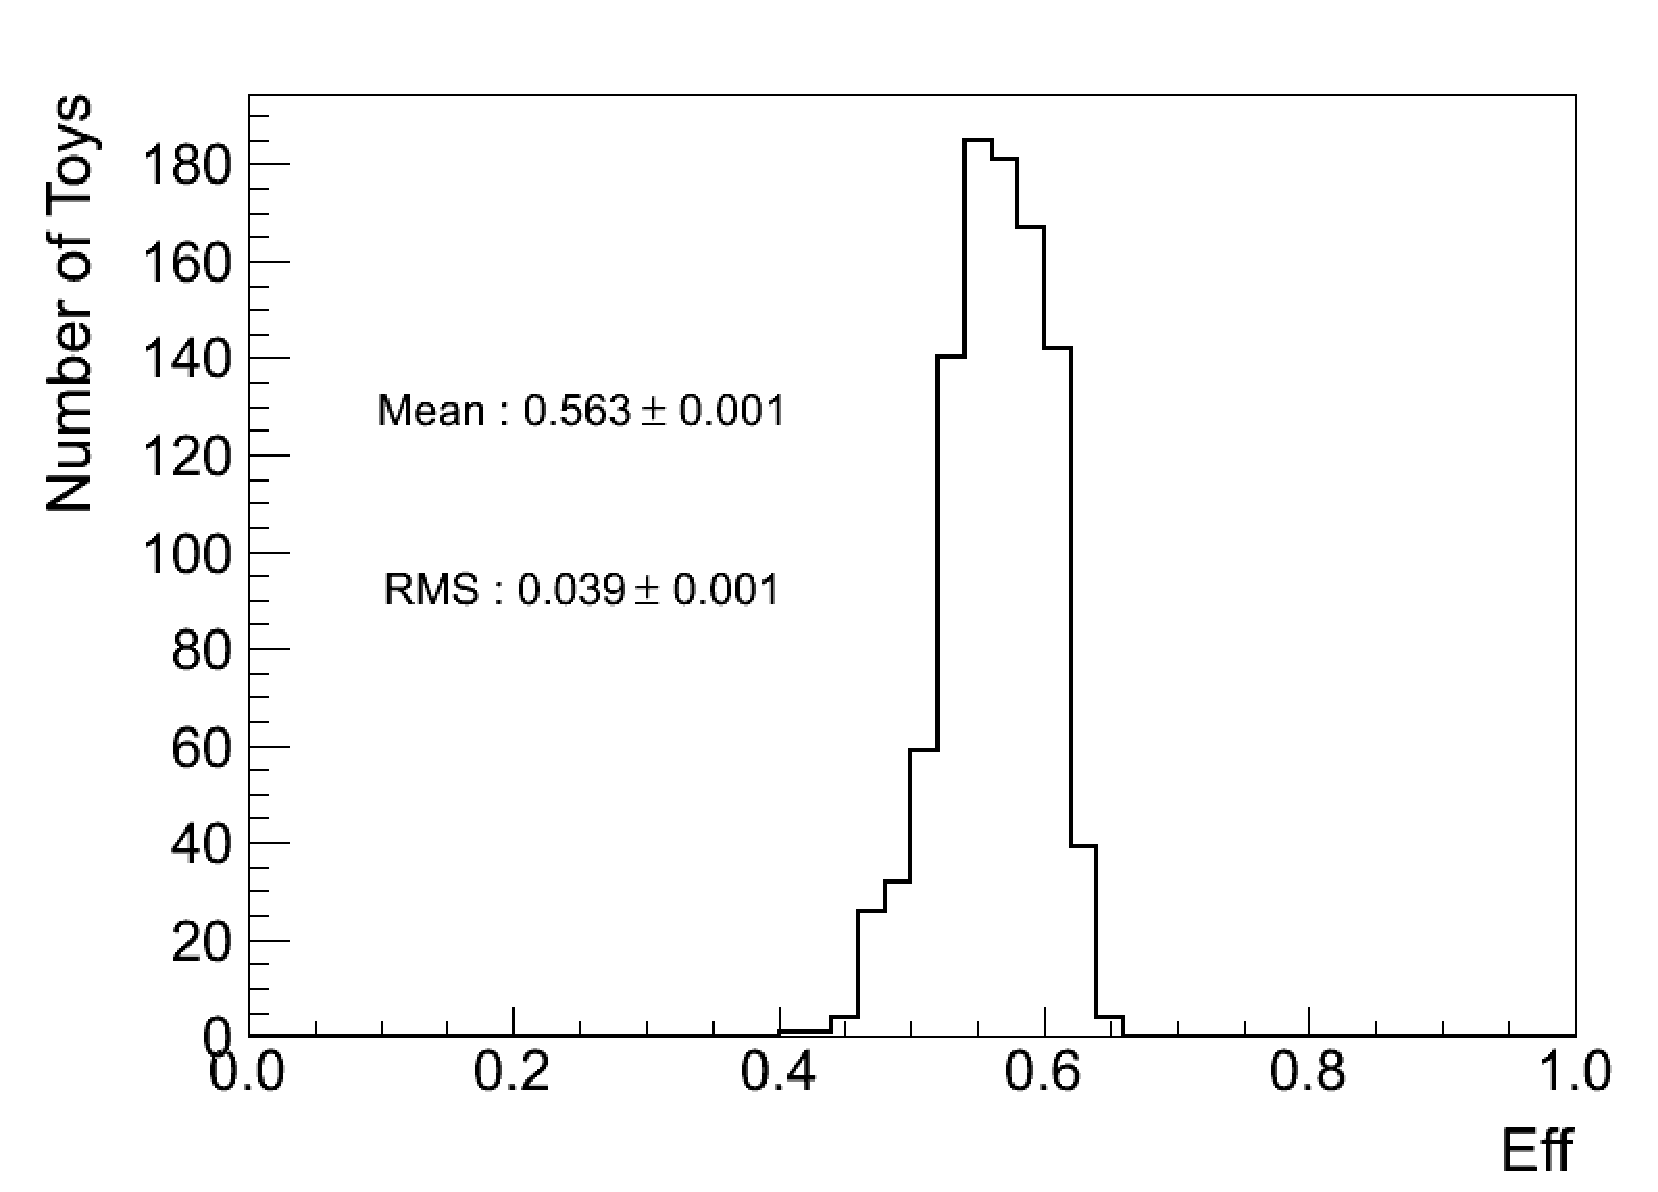
\includegraphics[width=0.48\textwidth]{figures/Eff_ShiftPlus1GeV.pdf}}
    \caption{The distribution of the fitted efficiency from sets of toys experiments are shown. 
      Alternative models are used to throw the toy experiments, while the efficiency fits are 
      performed assuming the nominal model. Any deviation in the mean of these distributions
      represent a systematic bias if the given alternative model is the true model for the data.
    }
    \label{fig:EffToys}
  \end{center}
\end{figure}


\section{Conclusion}

We have described a new method for measuring the selection efficiency for electrons with transverse
momentum below $20$~\GeV\ using \ZToEEGamma\ events. The signal to background in the failing sample
is enhanced up to about $10:1$ after all selection requirements, leading to a very clean measurement
of the efficiency even for electrons between $7$~\GeV\ and $10$~\GeV . For the \HiggsToZZ\ electron
selection used for the ICHEP 2012 analysis, we observe scale factors of about $0.8$ and $0.7$ for
barrel and endcap electrons repsectively in the $p_{T}$ range between $7$~\GeV\ and $10$~\GeV. 
For electrons in the $p_{T}$ range between $10$~\GeV\ and $20$~\GeV , we measure scale factors
consistent with $1.0$. 


%===================================================================================================
\clearpage

\vspace*{-0.2cm}
\thebibliography{12}

\bibitem{Item1}
 

%===================================================================================================

\appendix
\appendixpage

\section{Efficiency for 2011 Data}

 \begin{table}[!ht]
 \begin{center} 
 \begin{tabular}{|c|c|c|c|}
 \hline
 $p_{T}$ / $\eta$ bin    &  Monte Carlo Efficiency    &  Data Efficiency   &  MC to Data Scale Factor \\   \hline           
$  7.0 < p_{T} \le  10.0$ , $  0.0  \le |\eta| <   1.5$   &       0.7094 +/- 0.0186   &       0.6022 +/- 0.0460   &       0.8489 +/- 0.0685   \\   
\hline
$  7.0 < p_{T} \le  10.0$ , $  1.5  \le |\eta| <   2.5$   &       0.6534 +/- 0.0395   &       0.4744 +/- 0.0633   &       0.7260 +/- 0.1063   \\   
\hline
%$ 10.0 < p_{T} \le  15.0$ , $  0.0  \le |\eta| <   1.5$   &       0.8675 +/- 0.0081   &       0.8392 +/- 0.0172   &       0.9674 +/- 0.0218   \\   
%\hline
%$ 10.0 < p_{T} \le  15.0$ , $  1.5  \le |\eta| <   2.5$   &       0.8024 +/- 0.0194   &       0.7641 +/- 0.0437   &       0.9523 +/- 0.0592   \\   
%\hline
%$ 15.0 < p_{T} \le  20.0$ , $  0.0  \le |\eta| <   1.5$   &       0.9235 +/- 0.0061   &       0.9103 +/- 0.0119   &       0.9857 +/- 0.0145   \\   
%\hline
%$ 15.0 < p_{T} \le  20.0$ , $  1.5  \le |\eta| <   2.5$   &       0.8927 +/- 0.0147   &       0.8176 +/- 0.0323   &       0.9159 +/- 0.0392   \\   
%\hline
\end{tabular}
\caption{The efficiencies for the electron selection used in the \HiggsToZZ\ analysis for ICHEP 2012
measured from the Monte Carlo simulation and the 2011 data, and the Monte Carlo
to data scale factors are shown for different bins of $p_{T}$ and $\eta$. }
\label{tab:Efficiency_HZZICHEP2012WP_Data2011}
\end{center}
\end{table}


\begin{figure}[htb]
  \begin{center}
    \subfigure[Barrel Pass]{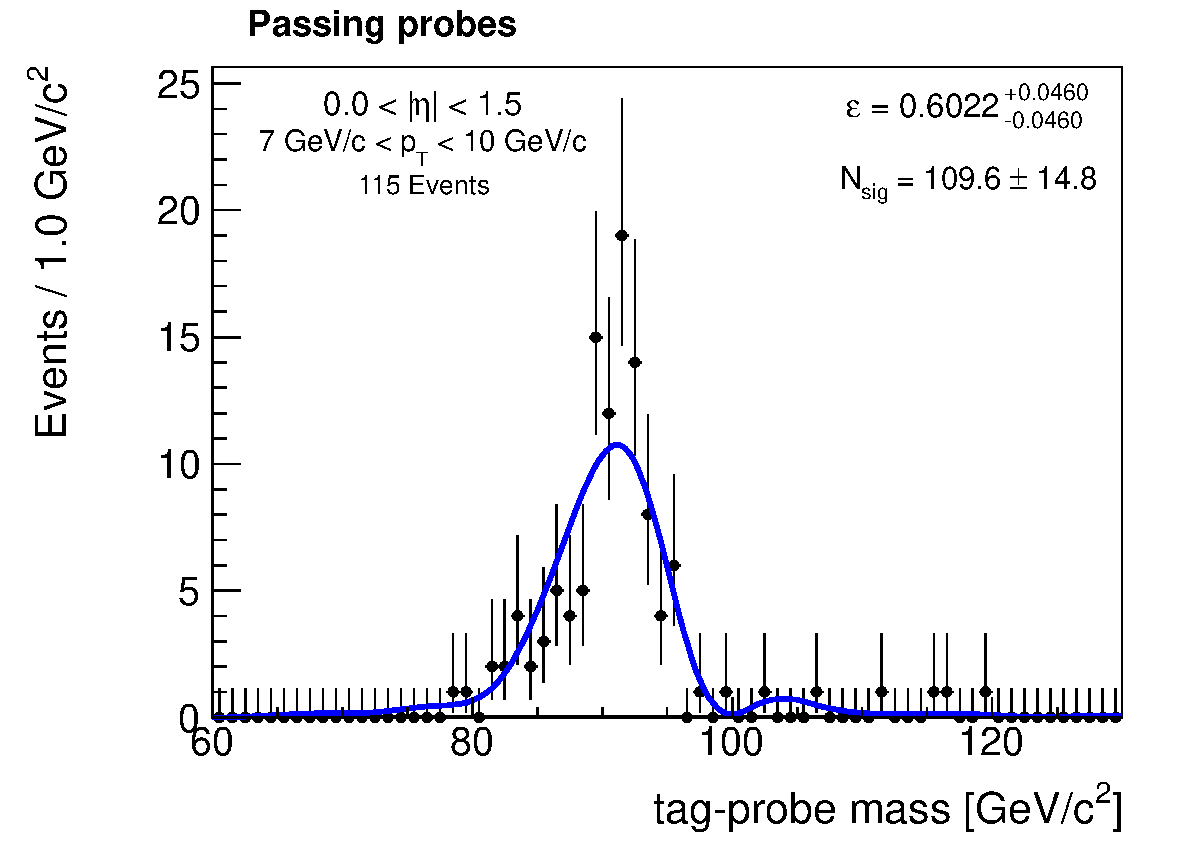
\includegraphics[width=0.48\textwidth]{figures/passetapt_TemplateConvGausPlusExpFit_Data2011_0.pdf}}
    \subfigure[Barrel Fail]{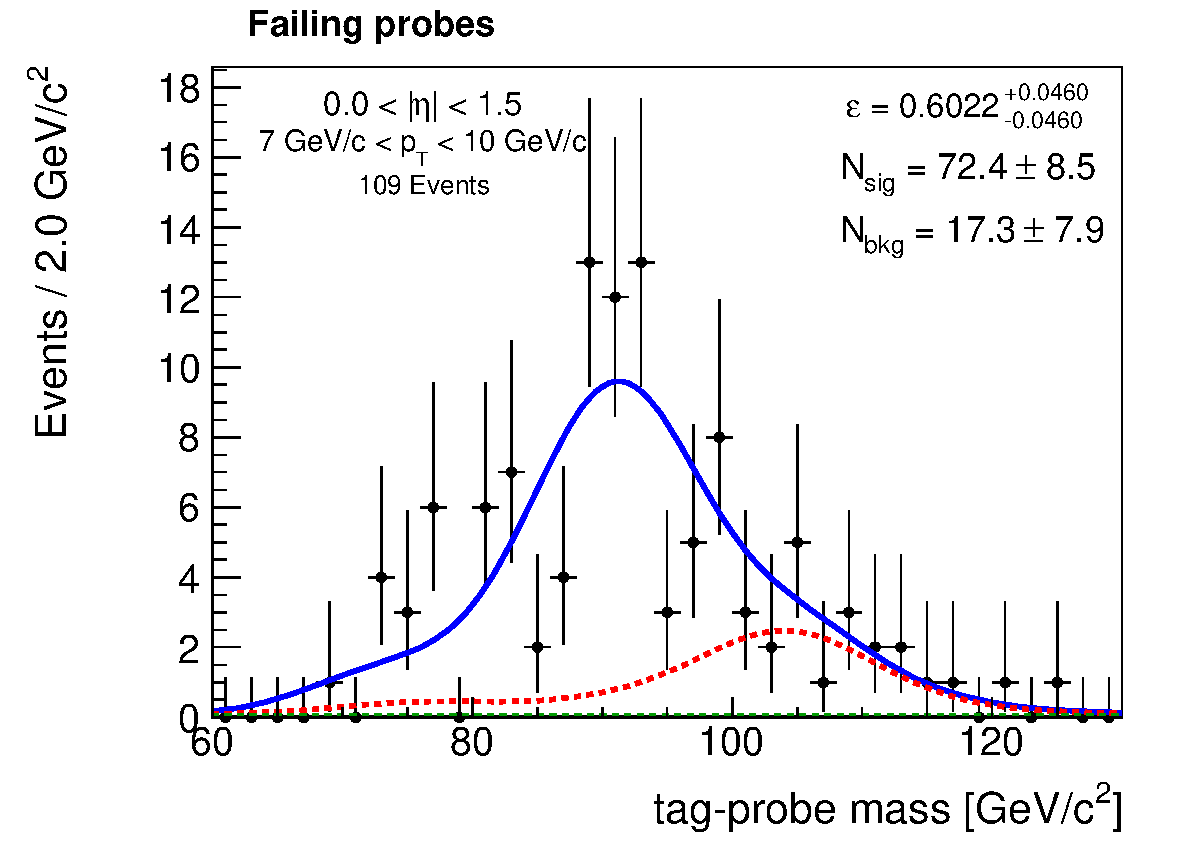
\includegraphics[width=0.48\textwidth]{figures/failetapt_TemplateConvGausPlusExpFit_Data2011_0.pdf}}
    \subfigure[Endcap Pass]{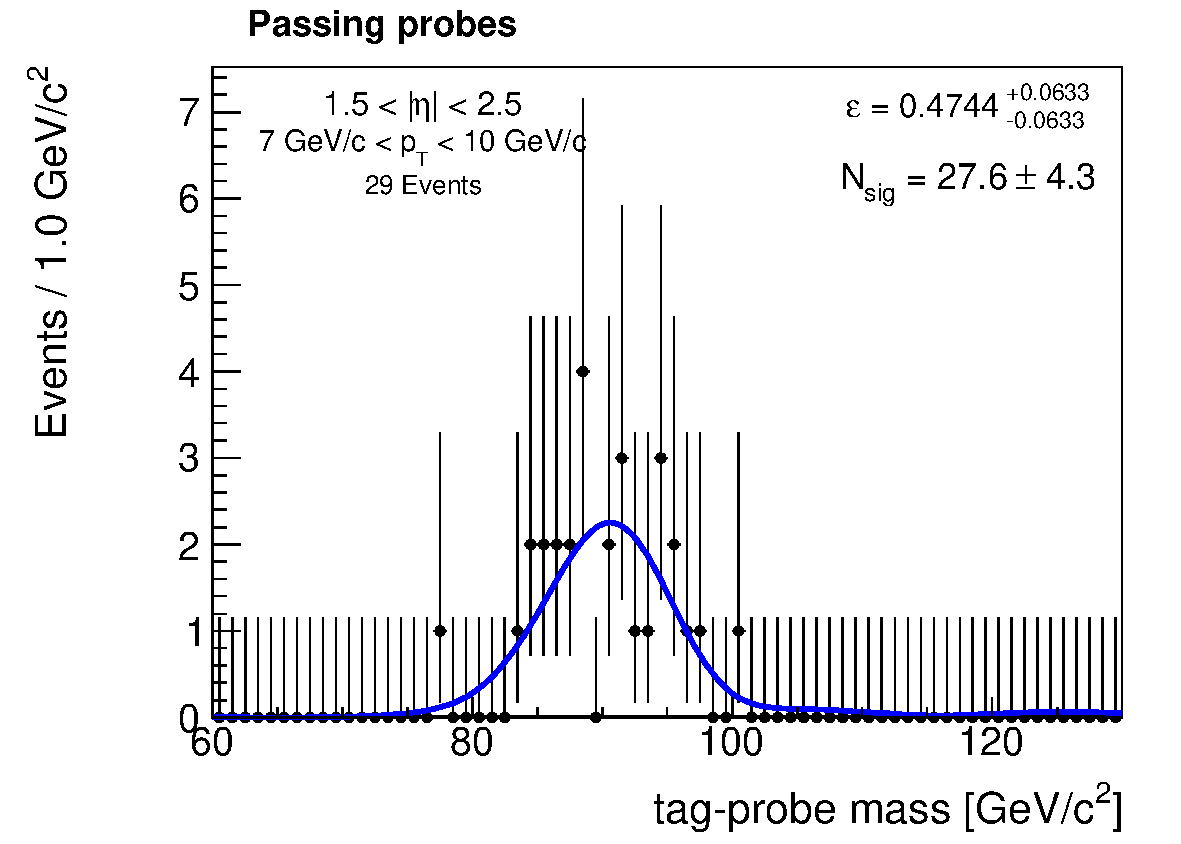
\includegraphics[width=0.48\textwidth]{figures/passetapt_TemplateConvGausPlusExpFit_Data2011_1.pdf}}
    \subfigure[Endcap Fail]{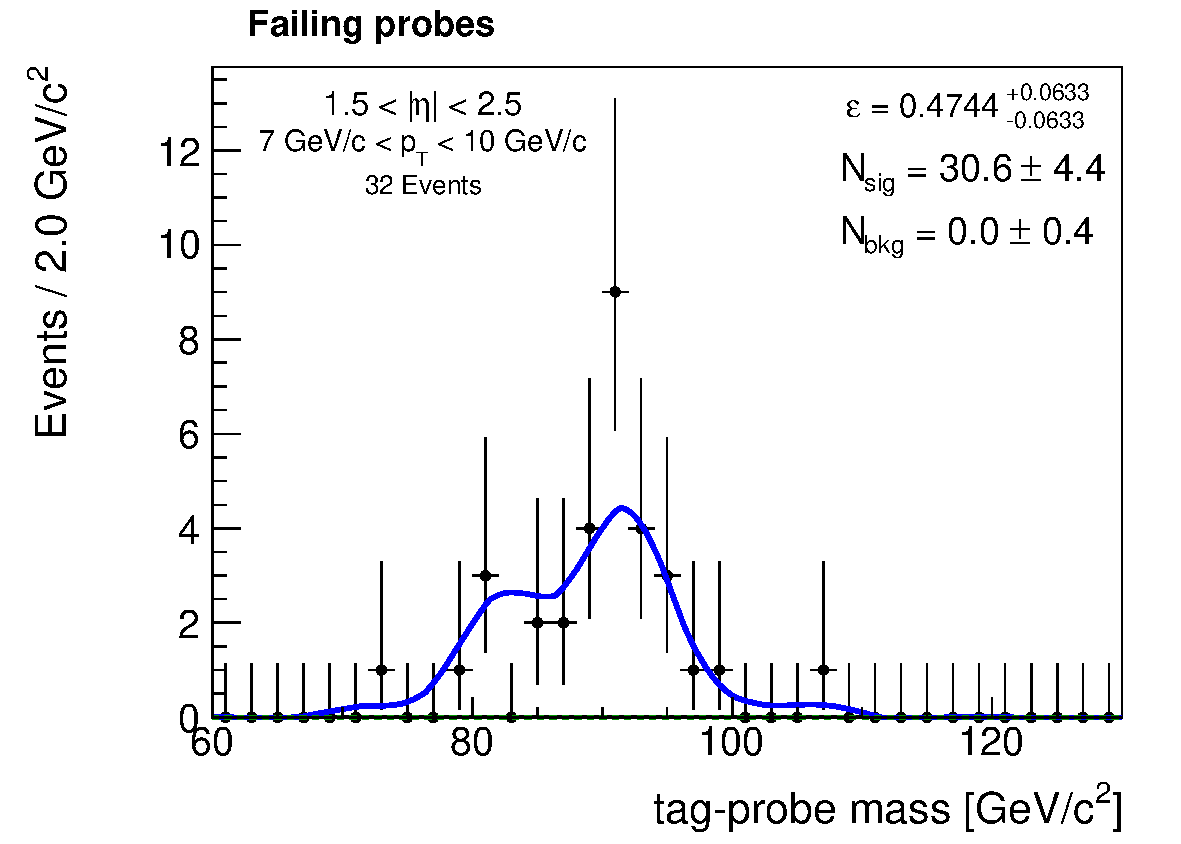
\includegraphics[width=0.48\textwidth]{figures/failetapt_TemplateConvGausPlusExpFit_Data2011_1.pdf}}
    \caption{Fits to the $m_{ee\gamma}$ distribution in 2011 data are shown for the pass and fail samples for
      electron probes with $p_{T}$ between $7$~\GeV\ and $10$~\GeV.
    }
    \label{fig:MassFits_Pt7To10_Data2011}
  \end{center}
\end{figure}


\section{Update for HCP 2012 Dataset}


 \begin{table}[!ht]
 \begin{center} 
 \begin{tabular}{|c|c|c|c|}
 \hline
 $p_{T}$ / $\eta$ bin    &  Monte Carlo Efficiency    &  Data Efficiency   &  MC to Data Scale Factor \\   \hline           
$  7.0 < p_{T} \le  10.0$ , $  0.0  \le |\eta| <   1.5$   &       0.6725 +/- 0.0302   &       0.5017 +/- 0.0271   &       0.7459 +/- 0.0524   \\   
\hline
$  7.0 < p_{T} \le  10.0$ , $  1.5  \le |\eta| <   2.5$   &       0.5783 +/- 0.0609   &       0.4033 +/- 0.0550   &       0.6974 +/- 0.1201   \\   
\hline
\end{tabular}
\caption{ Efficiency for the selection used for the HZZ analysis for the HCP 2012 conference, measured on the HCP dataset of the 2012 data }
\label{tab:Efficiency_HZZICHEP2012WP_HCP2012}
\end{center}
\end{table}

\begin{figure}[htb]
  \begin{center}
    \subfigure[Barrel Pass]{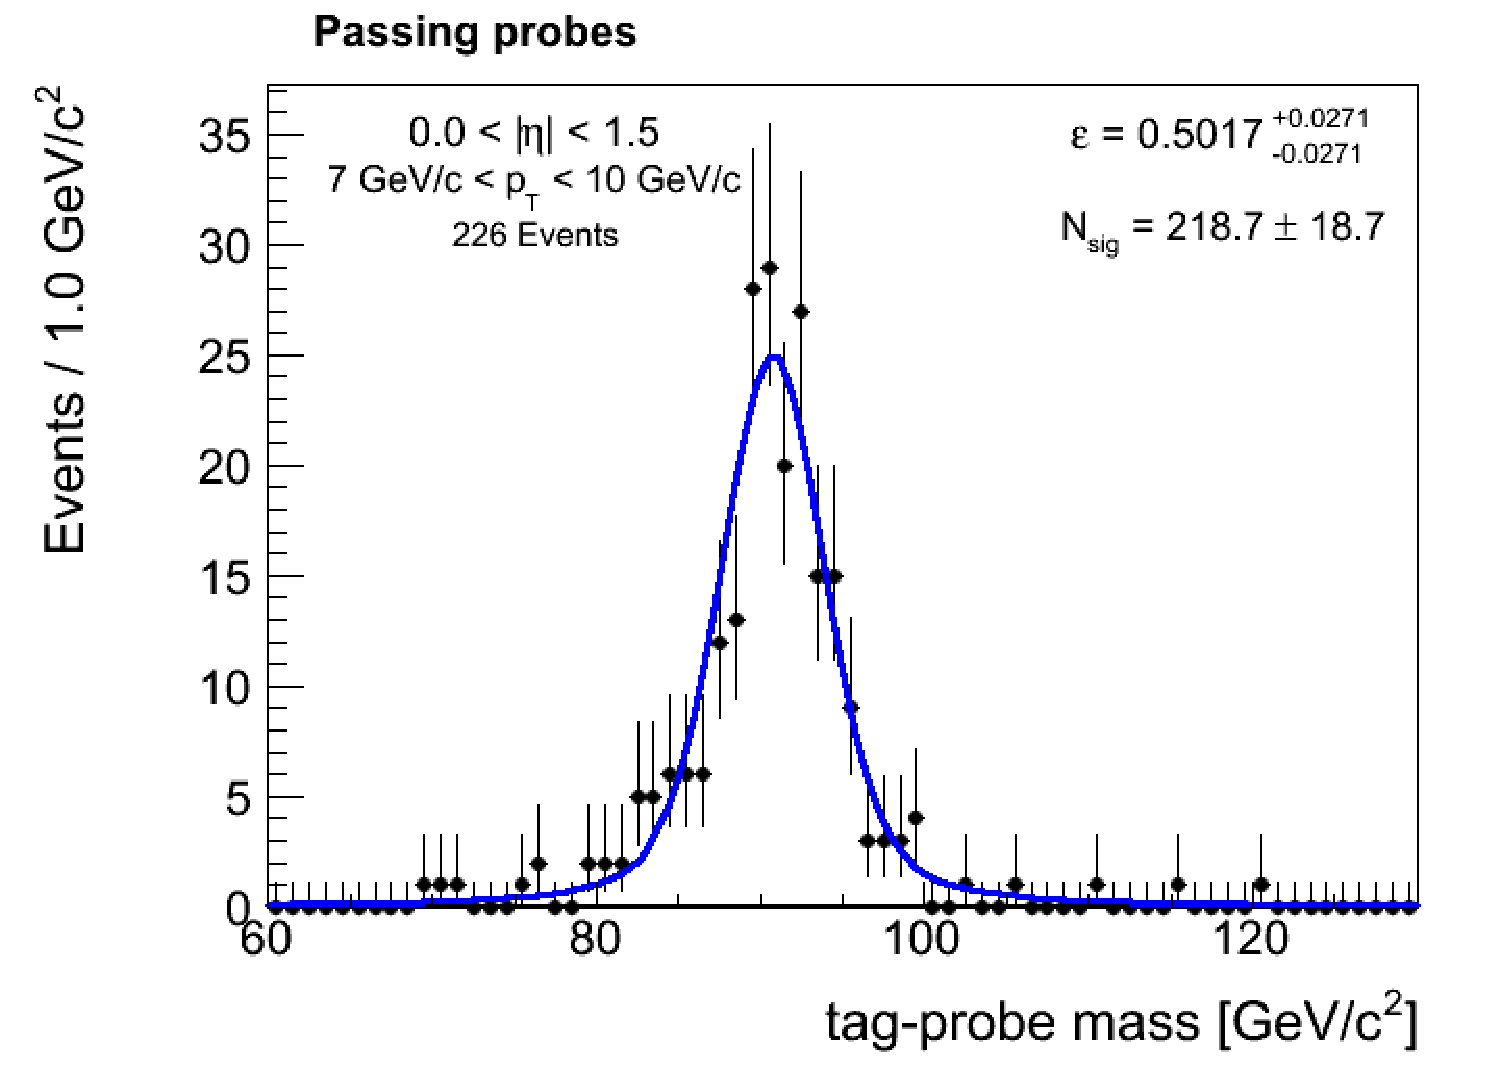
\includegraphics[width=0.48\textwidth]{figures/passetapt_EleHZZHCP2012WP_TemplateConvGausPlusExpFit_DataHCP2012_0.pdf}}
    \subfigure[Barrel Fail]{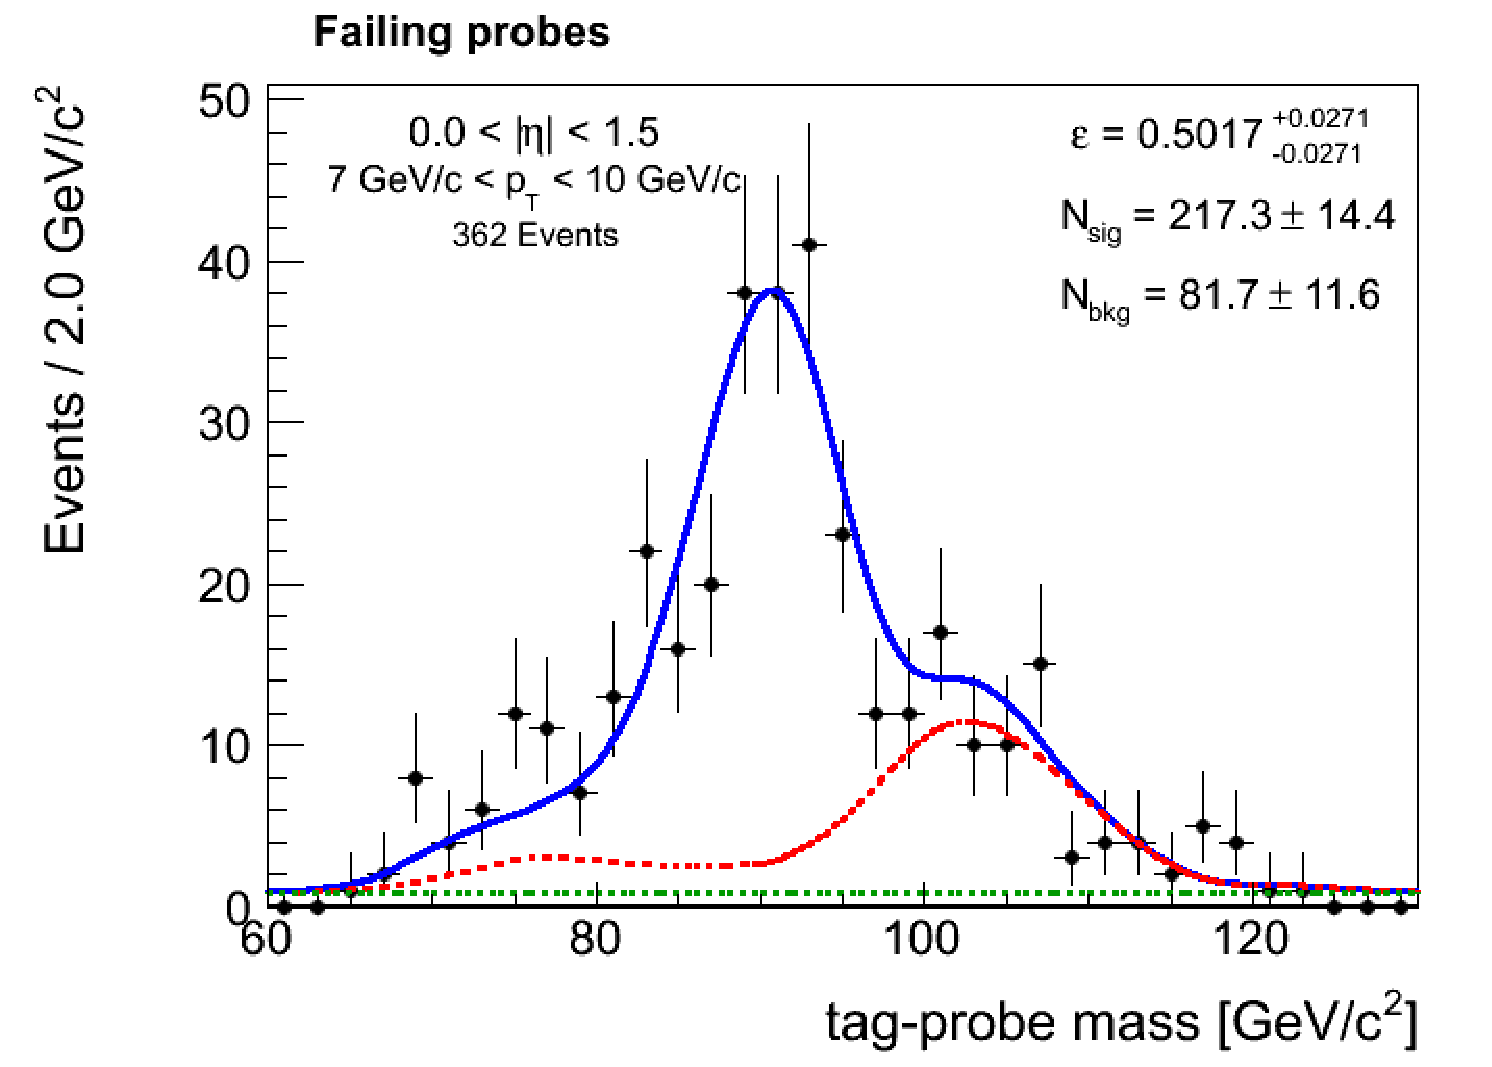
\includegraphics[width=0.48\textwidth]{figures/failetapt_EleHZZHCP2012WP_TemplateConvGausPlusExpFit_DataHCP2012_0.pdf}}
    \subfigure[Endcap Pass]{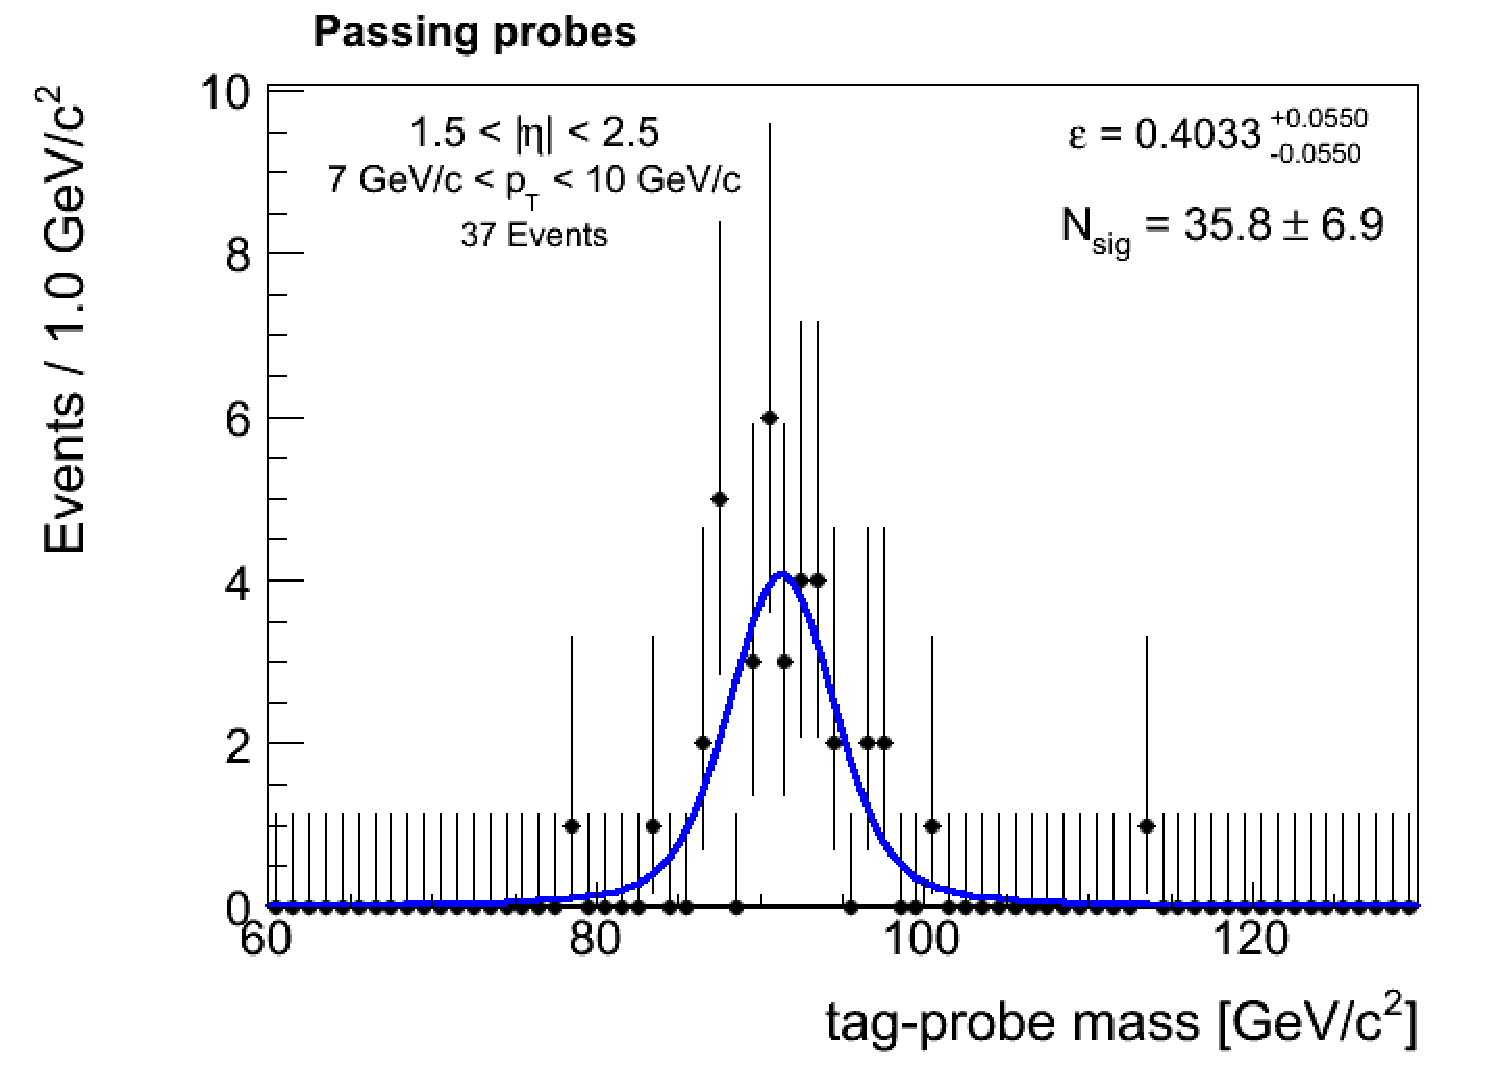
\includegraphics[width=0.48\textwidth]{figures/passetapt_EleHZZHCP2012WP_TemplateConvGausPlusExpFit_DataHCP2012_1.pdf}}
    \subfigure[Endcap Fail]{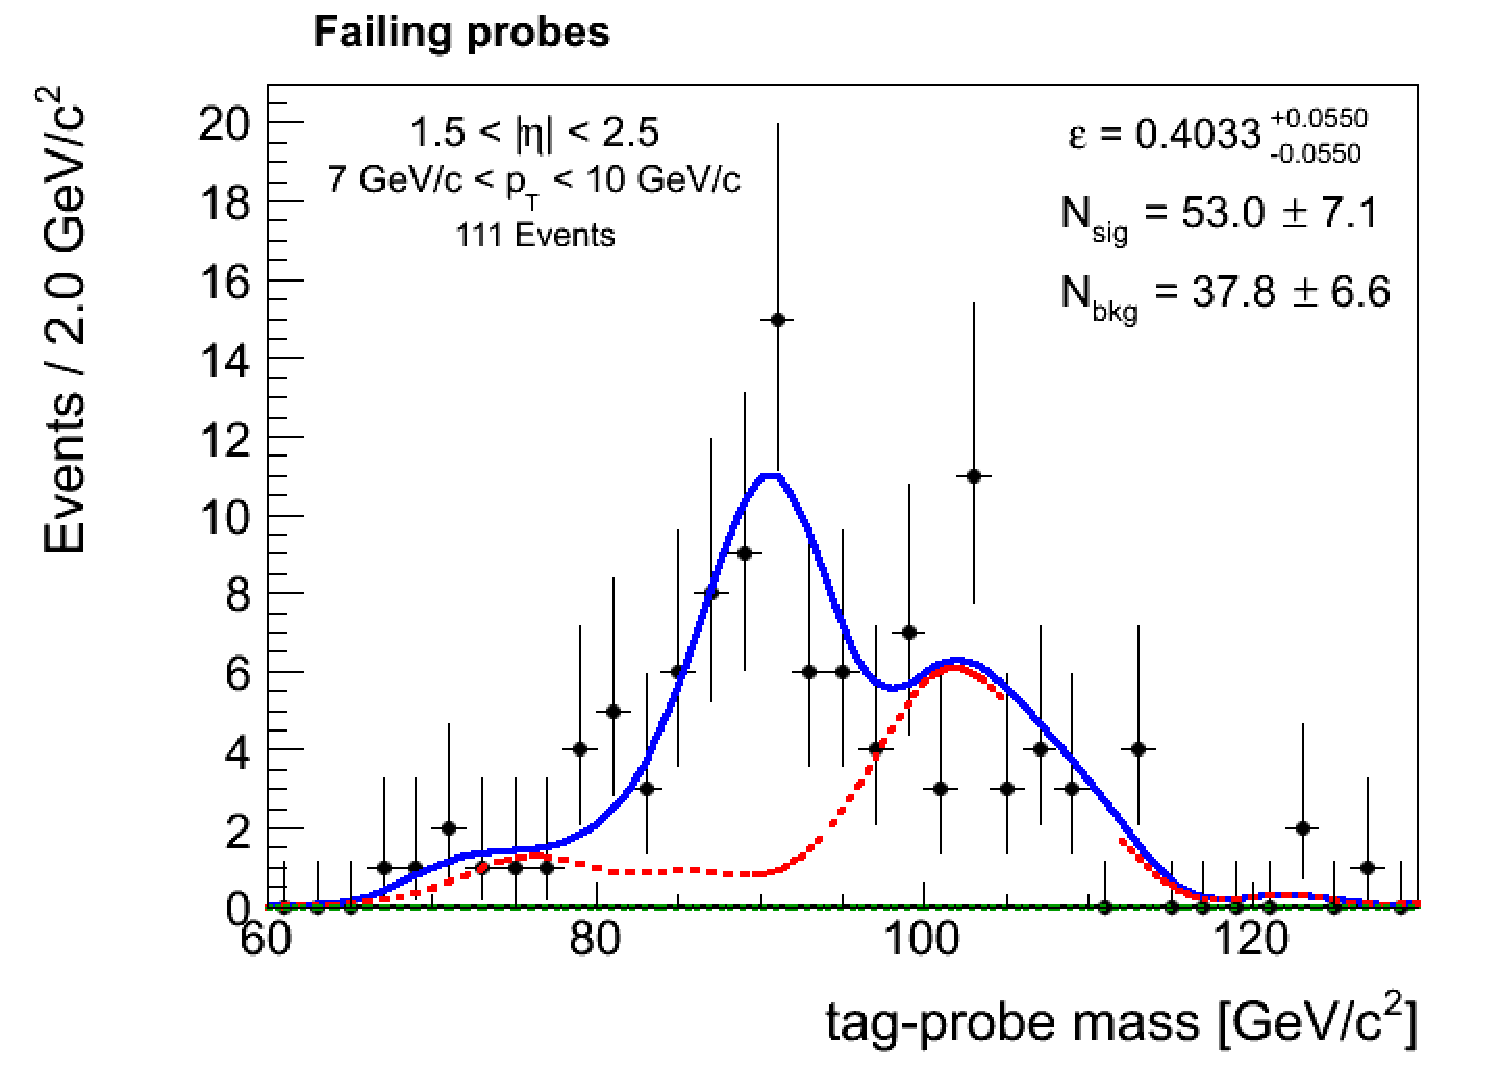
\includegraphics[width=0.48\textwidth]{figures/failetapt_EleHZZHCP2012WP_TemplateConvGausPlusExpFit_DataHCP2012_1.pdf}}
    \caption{Fits to the $m_{ee\gamma}$ distribution from the 2012 data with the HCP dataset are shown for the pass and fail samples 
      for electron probes with $p_{T}$ between $7$~\GeV\ and $10$~\GeV used to measure the efficiency of the HZZ electron selection.
    }
    \label{fig:EleEffMassFits_HZZHCP2012WP_Pt7To10_ZeeGamma_HCP2012}
  \end{center}
\end{figure}



 \begin{table}[!ht]
 \begin{center} 
 \begin{tabular}{|c|c|c|c|}
 \hline
 $p_{T}$ / $\eta$ bin    &  Monte Carlo Efficiency    &  Data Efficiency   &  MC to Data Scale Factor \\   \hline           
$  7.0 < p_{T} \le  10.0$ , $  0.0  \le |\eta| <   1.5$   &       0.8056 +/- 0.0262   &       0.7177 +/- 0.0270   &       0.8909 +/- 0.0443   \\   
\hline
$  7.0 < p_{T} \le  10.0$ , $  1.5  \le |\eta| <   2.5$   &       0.8452 +/- 0.0499   &       0.8476 +/- 0.0424   &       1.0028 +/- 0.0776   \\   
\hline
\end{tabular}
\caption{ Efficiency for the isolation cuts in the selection used for the HZZ analysis for the HCP 2012 conference, 
  measured on the HCP dataset of the 2012 data  }
\label{tab:Efficiency_HZZICHEP2012Iso_HCP2012}
\end{center}
\end{table}


\begin{figure}[htb]
  \begin{center}
    \subfigure[Barrel Pass]{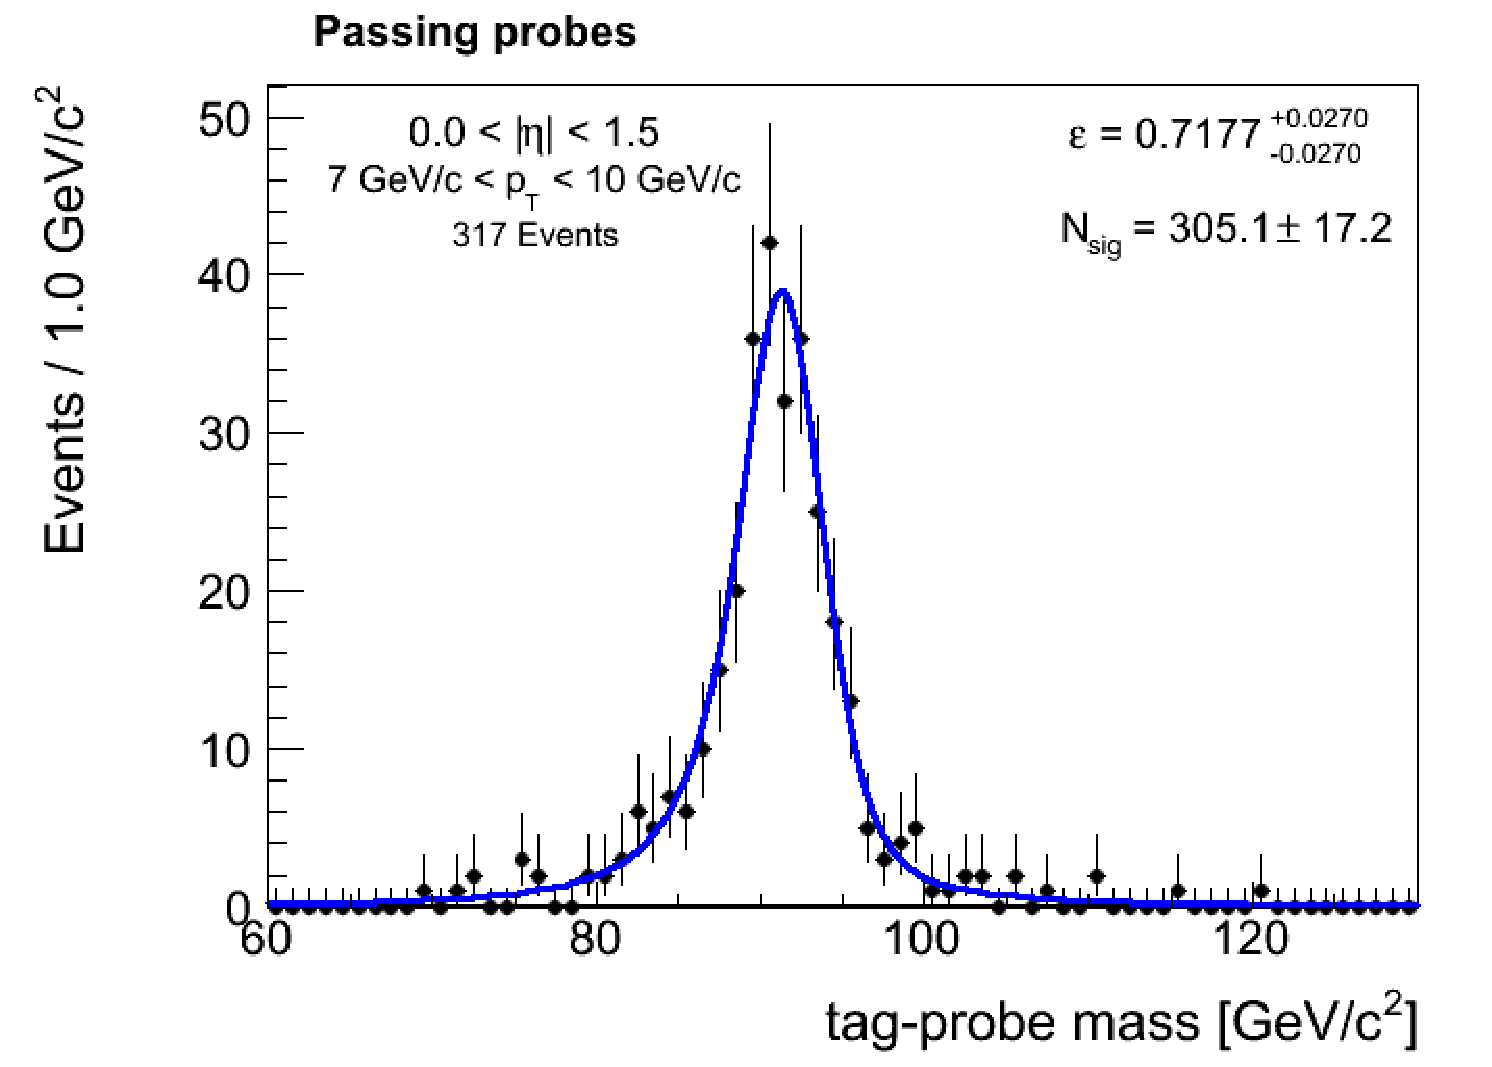
\includegraphics[width=0.48\textwidth]{figures/passetapt_EleHZZHCP2012IsoOnly_TemplateConvGausPlusExpFit_DataHCP2012_0.pdf}}
    \subfigure[Barrel Fail]{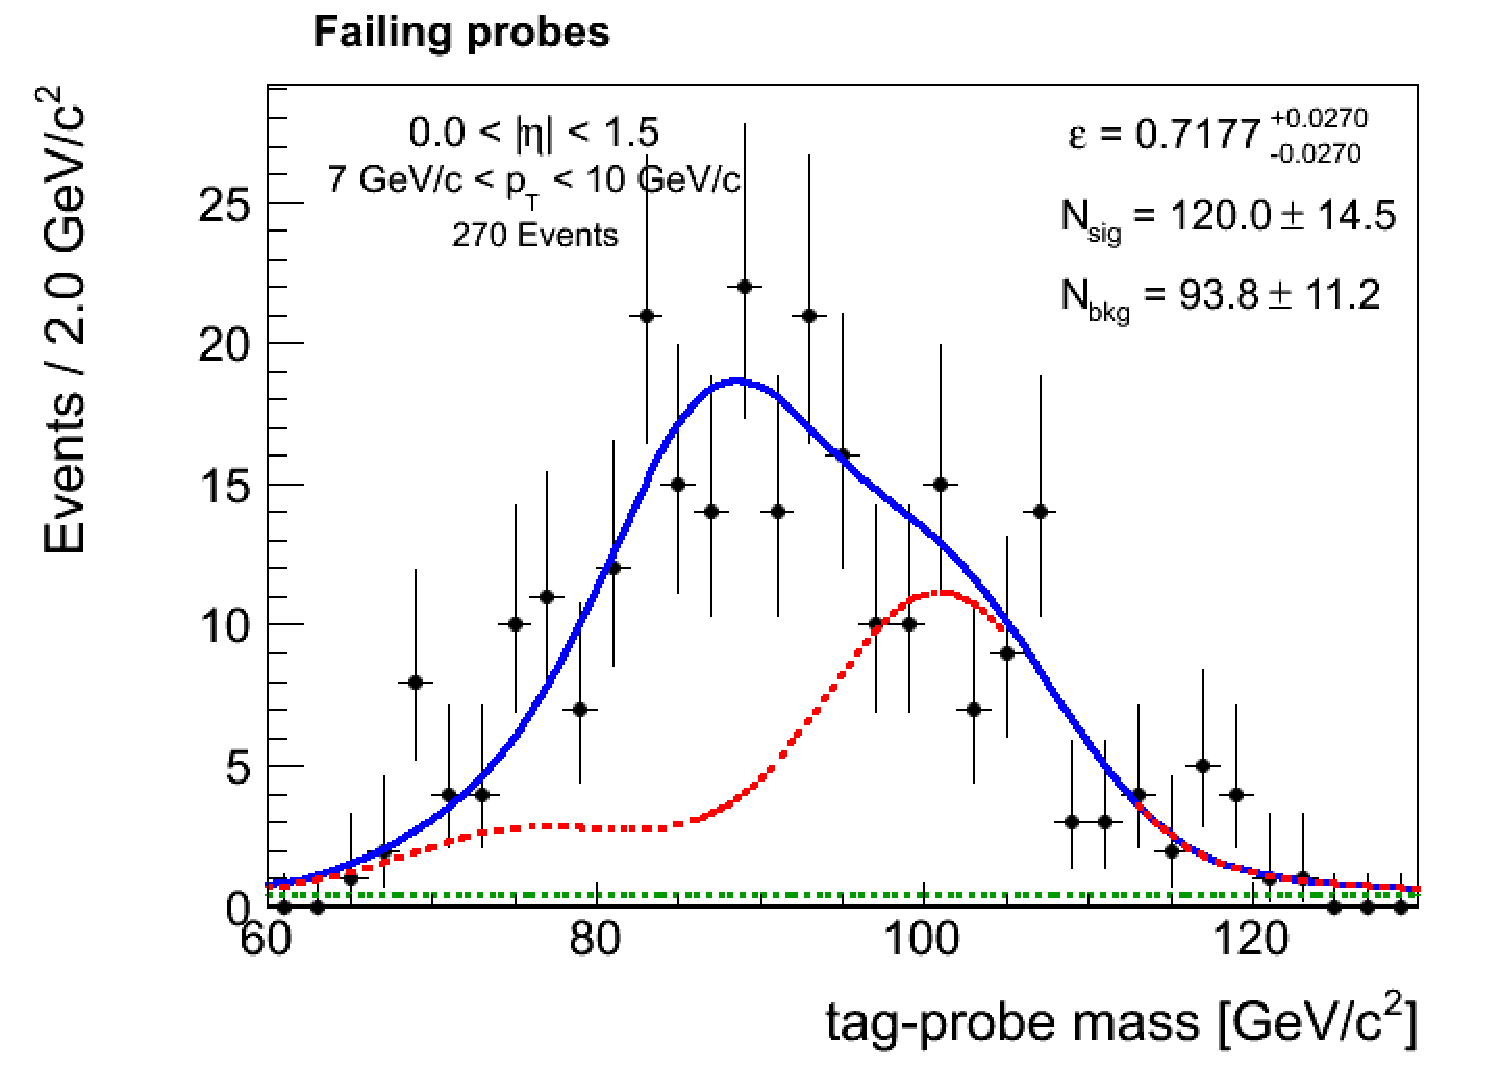
\includegraphics[width=0.48\textwidth]{figures/failetapt_EleHZZHCP2012IsoOnly_TemplateConvGausPlusExpFit_DataHCP2012_0.pdf}}
    \subfigure[Endcap Pass]{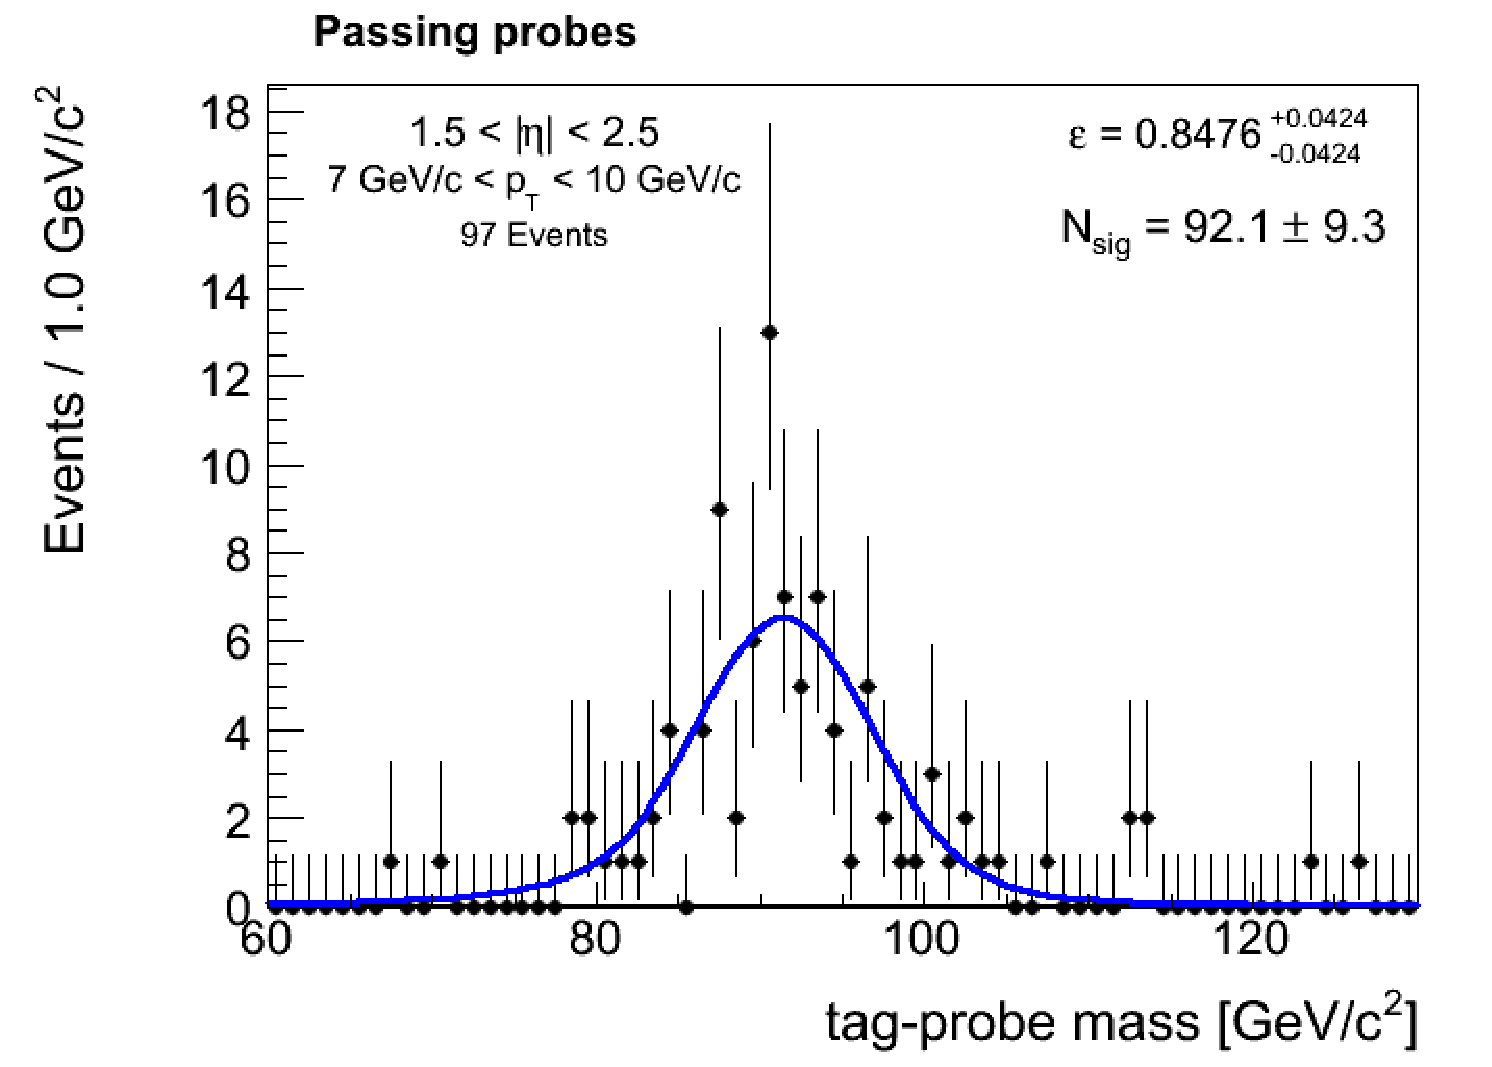
\includegraphics[width=0.48\textwidth]{figures/passetapt_EleHZZHCP2012IsoOnly_TemplateConvGausPlusExpFit_DataHCP2012_1.pdf}}
    \subfigure[Endcap Fail]{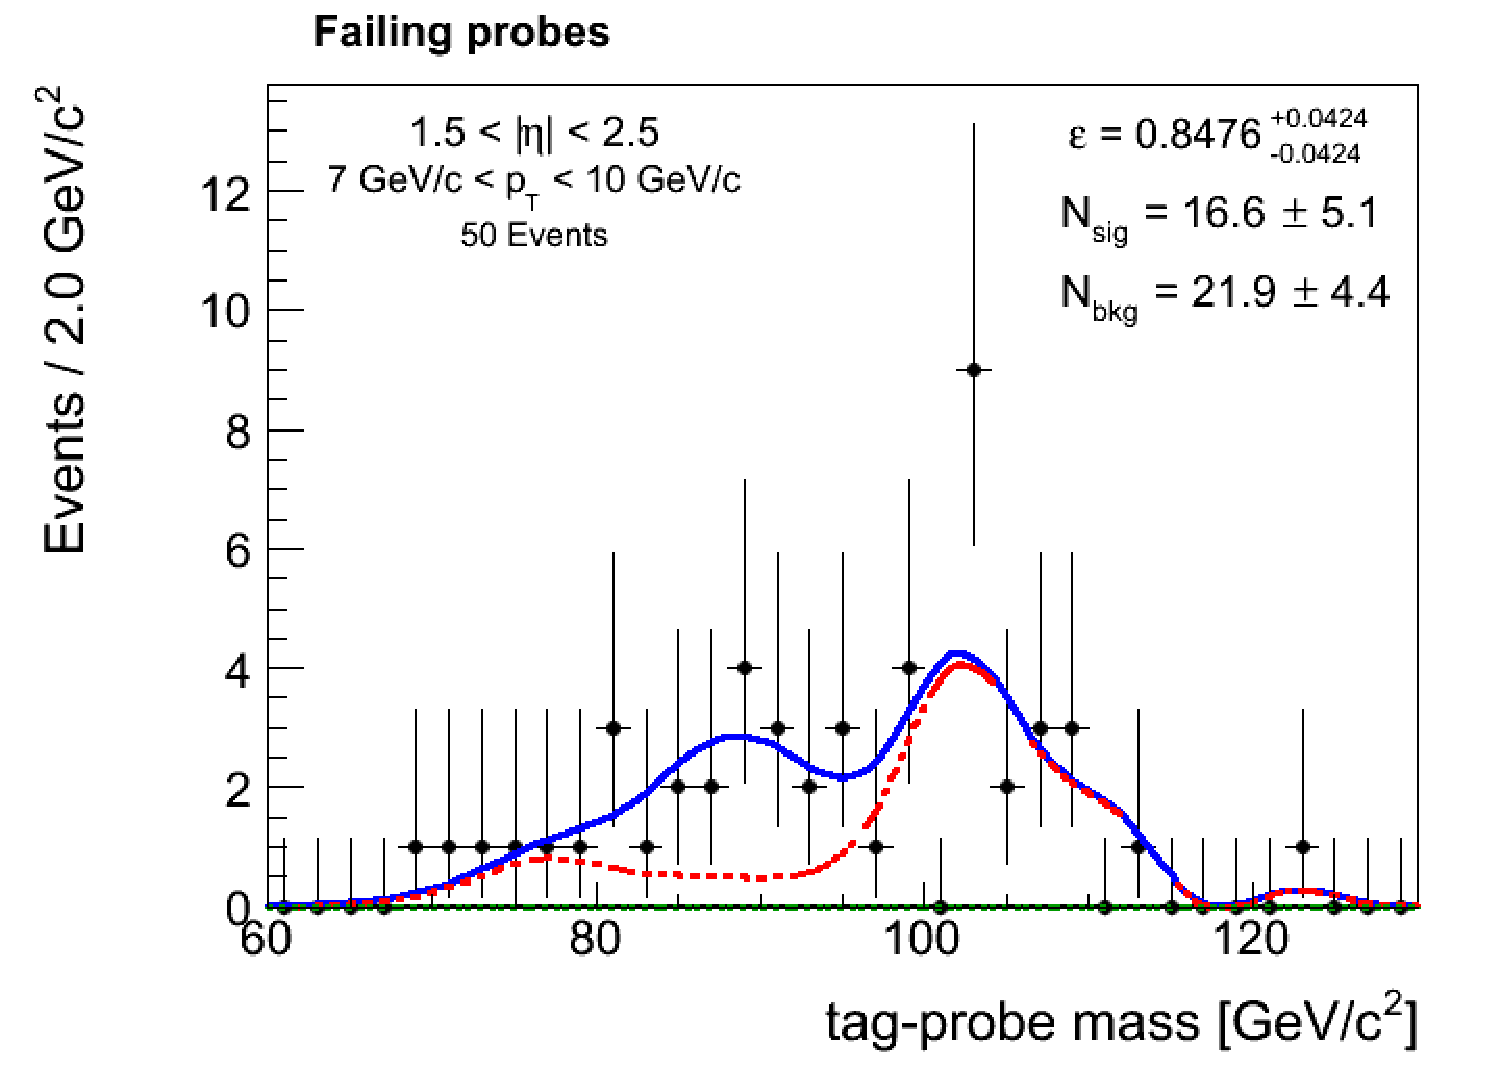
\includegraphics[width=0.48\textwidth]{figures/failetapt_EleHZZHCP2012IsoOnly_TemplateConvGausPlusExpFit_DataHCP2012_1.pdf}}
    \caption{Fits to the $m_{ee\gamma}$ distribution from the 2012 data with the HCP dataset are shown for the pass and fail samples for
      electron probes with $p_{T}$ between $7$~\GeV\ and $10$~\GeV used to measure the isolation efficiency of the HZZ electron selection.
    }
    \label{fig:MassFits_Pt7To10_Data2011}
  \end{center}
\end{figure}



 \begin{table}[!ht]
 \begin{center} 
 \begin{tabular}{|c|c|c|c|}
 \hline
 $p_{T}$ / $\eta$ bin    &  Monte Carlo Efficiency    &  Data Efficiency   &  MC to Data Scale Factor \\   \hline           
$  7.0 < p_{T} \le  10.0$ , $  0.0  \le |\eta| <   1.5$   &       0.8319 +/- 0.0282   &       0.7447 +/- 0.0281   &       0.8952 +/- 0.0454   \\   
\hline
$  7.0 < p_{T} \le  10.0$ , $  1.5  \le |\eta| <   2.5$   &       0.6901 +/- 0.0645   &       0.4810 +/- 0.0598   &       0.6969 +/- 0.1084   \\   
\hline
\end{tabular}
\caption{ Efficiency for the identification and impact parameter cuts in the selection used for the HZZ analysis
  for electrons already passing the isolation cuts for the HCP 2012 conference, 
  measured on the HCP dataset of the 2012 data  }
\label{tab:Efficiency_HZZICHEP2012IDGivenIso_HCP2012}
\end{center}
\end{table}



\begin{figure}[htb]
  \begin{center}
    \subfigure[Barrel Pass]{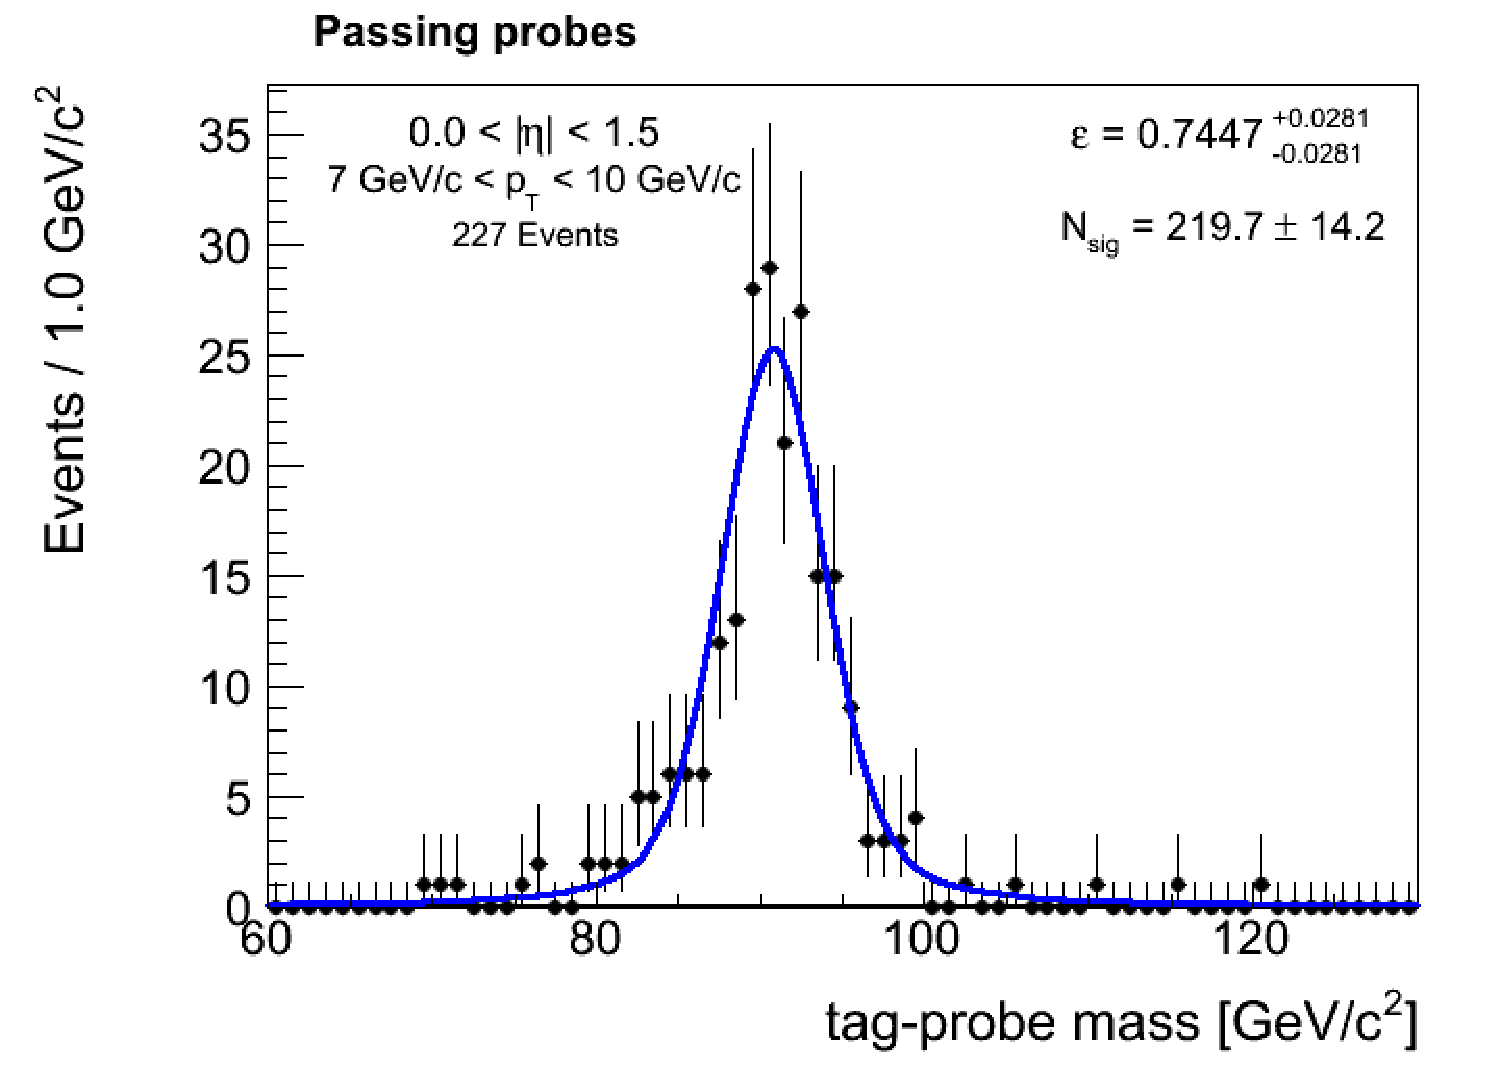
\includegraphics[width=0.48\textwidth]{figures/passetapt_EleHZZHCP2012IDGivenIso_TemplateConvGausPlusExpFit_DataHCP2012_0.pdf}}
    \subfigure[Barrel Fail]{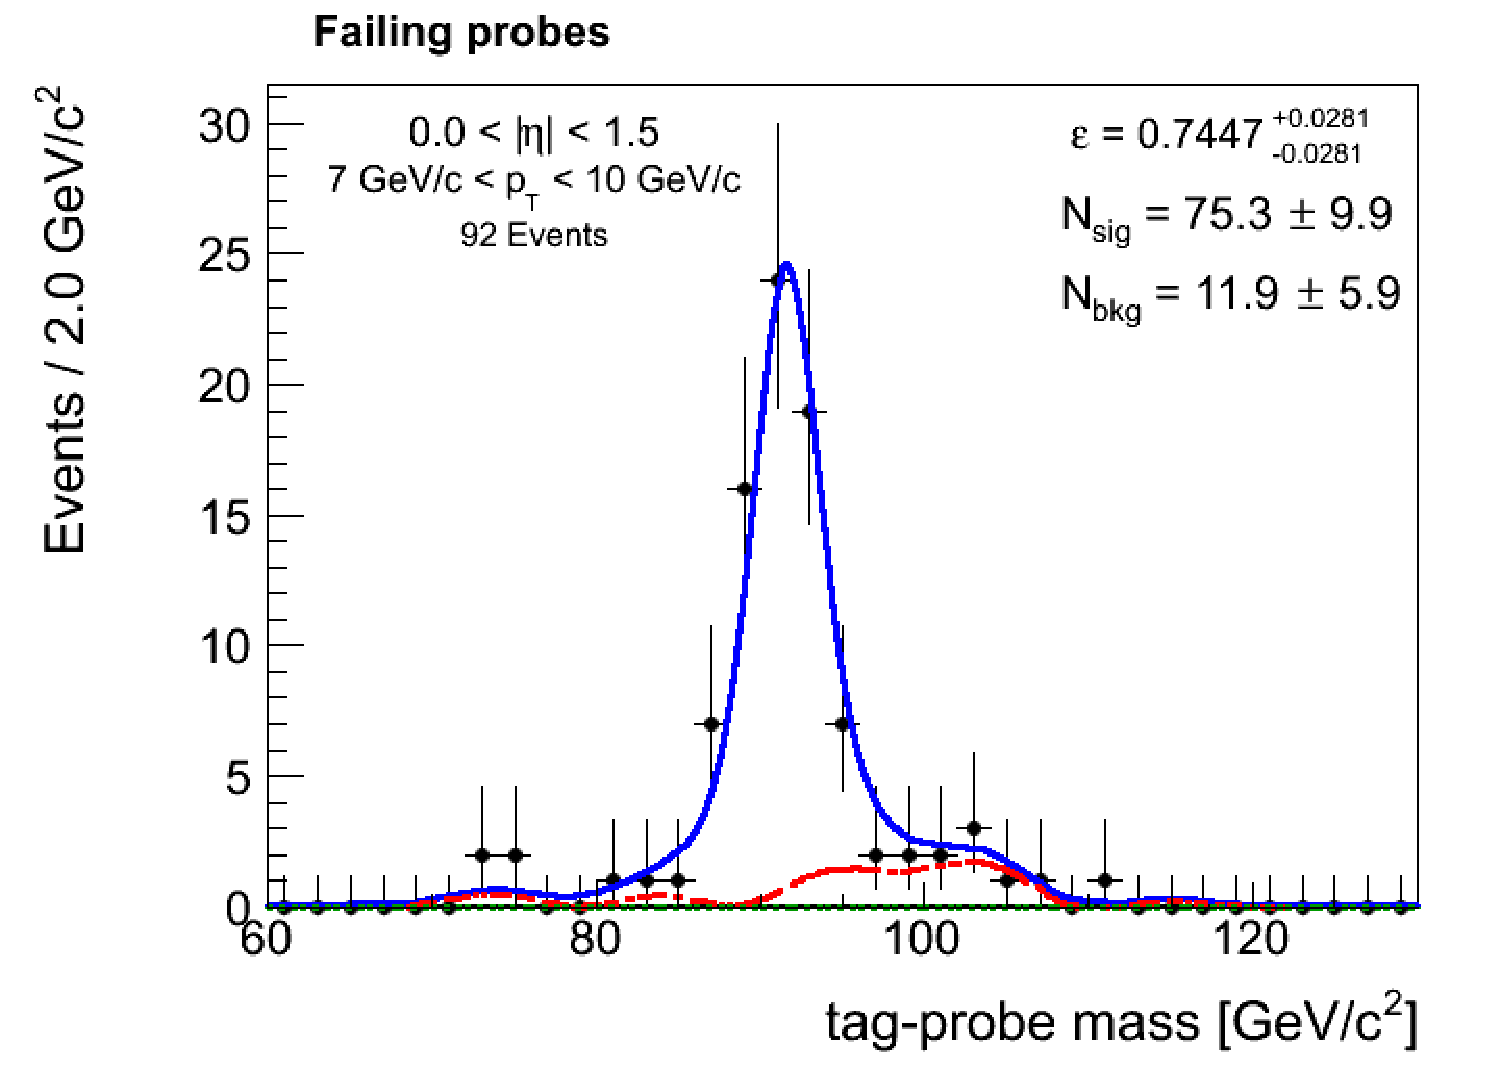
\includegraphics[width=0.48\textwidth]{figures/failetapt_EleHZZHCP2012IDGivenIso_TemplateConvGausPlusExpFit_DataHCP2012_0.pdf}}
    \subfigure[Endcap Pass]{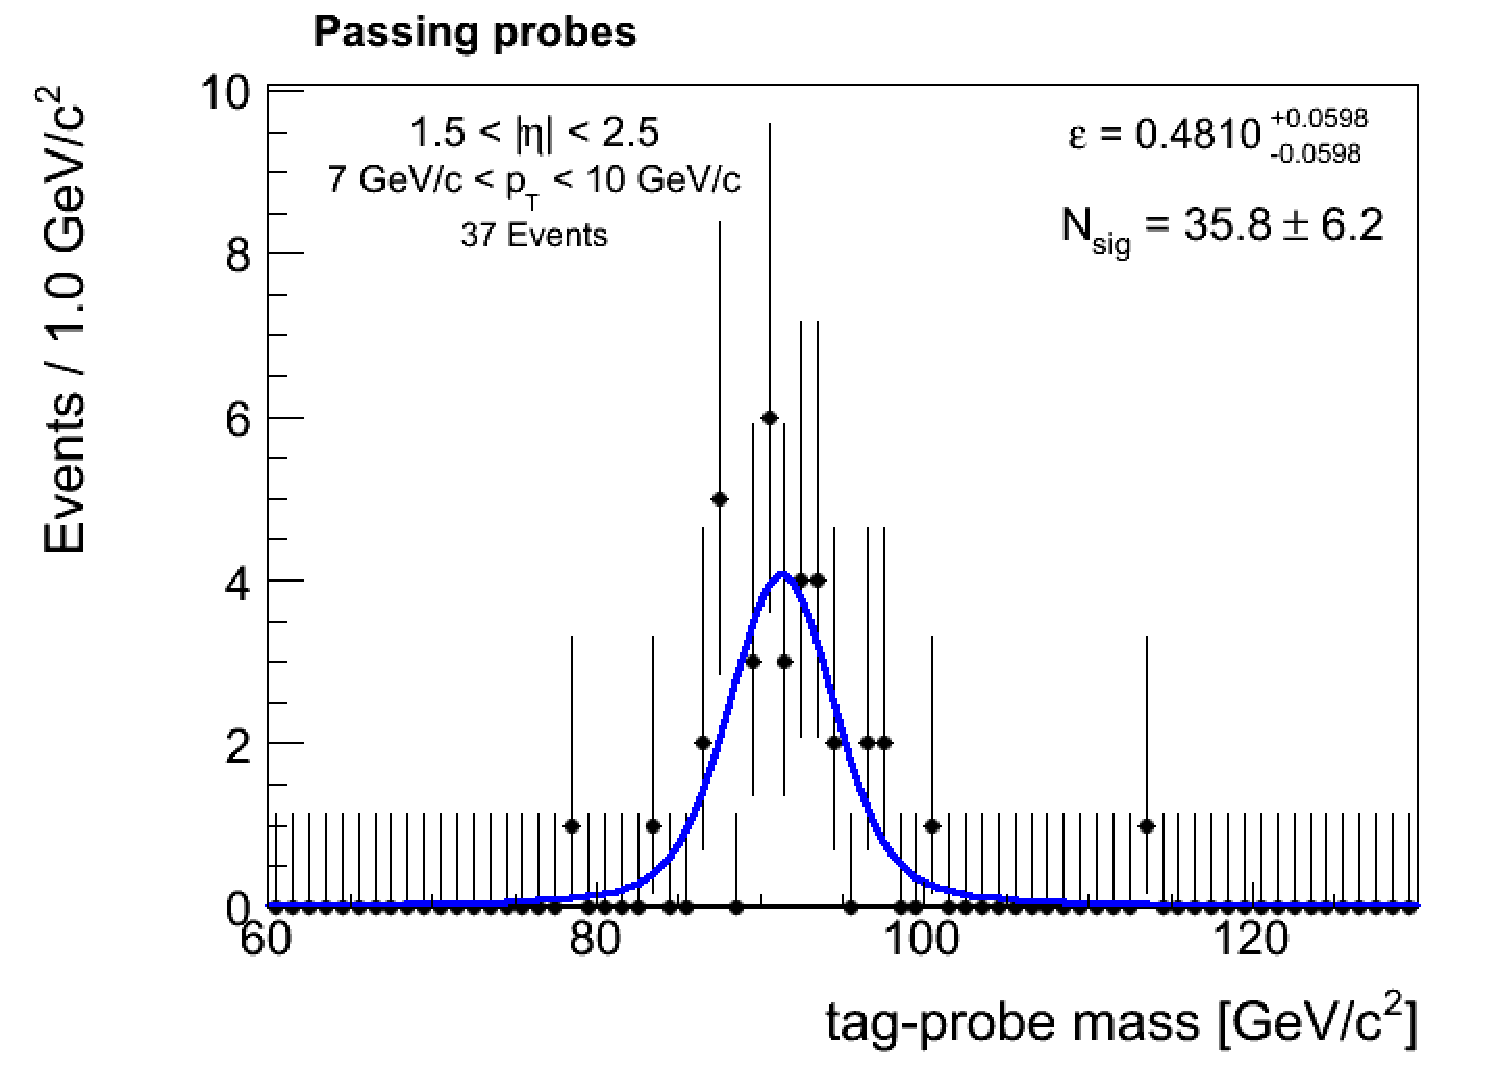
\includegraphics[width=0.48\textwidth]{figures/passetapt_EleHZZHCP2012IDGivenIso_TemplateConvGausPlusExpFit_DataHCP2012_1.pdf}}
    \subfigure[Endcap Fail]{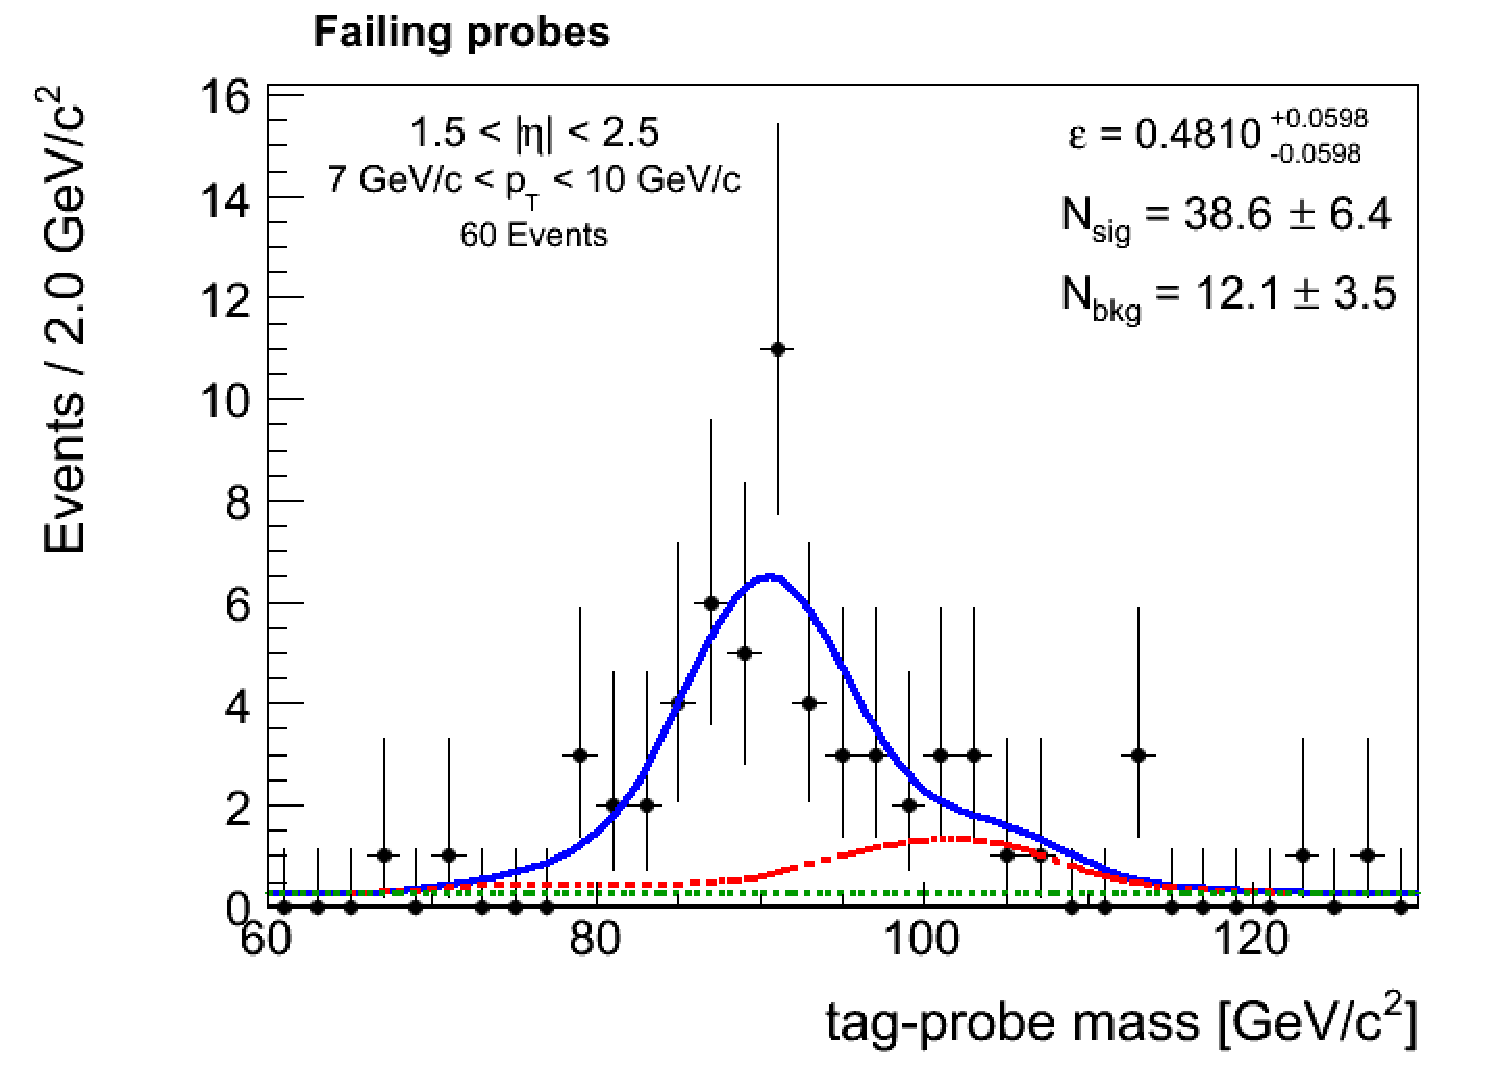
\includegraphics[width=0.48\textwidth]{figures/failetapt_EleHZZHCP2012IDGivenIso_TemplateConvGausPlusExpFit_DataHCP2012_1.pdf}}
    \caption{Fits to the $m_{ee\gamma}$ distribution from the 2012 data with the HCP dataset are shown for the pass and fail samples for
      electron probes with $p_{T}$ between $7$~\GeV\ and $10$~\GeV used to measure the identification and impact parameter 
      efficiency of the HZZ electron selection for electrons that already passed the isolation cuts.
    }
    \label{fig:MassFits_Pt7To10_Data2011}
  \end{center}
\end{figure}



%%%%%%%%%%%%%%%%%%%%%%%%%%%%%%%%%%%%%%%%%%%%%%%%%%%%%%%%%%%%
% Iso Given ID : just for cross check - not really used.
%%%%%%%%%%%%%%%%%%%%%%%%%%%%%%%%%%%%%%%%%%%%%%%%%%%%%%%%%%%%%

%%  \begin{table}[!ht]
%%  \begin{center} 
%%  \begin{tabular}{|c|c|c|c|}
%%  \hline
%%  $p_{T}$ / $\eta$ bin    &  Monte Carlo Efficiency    &  Data Efficiency   &  MC to Data Scale Factor \\   \hline           
%% $  7.0 < p_{T} \le  10.0$ , $  0.0  \le |\eta| <   1.5$   &       0.8248 +/- 0.0285   &       0.7985 +/- 0.0368   &       0.9682 +/- 0.0557   \\   
%% \hline
%% $  7.0 < p_{T} \le  10.0$ , $  1.5  \le |\eta| <   2.5$   &       0.8909 +/- 0.0595   &       0.9231 +/- 0.0990   &       1.0361 +/- 0.1309   \\   
%% \hline
%% \end{tabular}
%% \caption{ HCP HZZ selection Isolation Given ID, 2012 data, HCP Dataset }
%% \label{tab:Efficiency_HZZICHEP2012IsoGivenID_HCP2012}
%% \end{center}
%% \end{table}


%%%%%%%%%%%%%%%%%%%%%%%%%%%%%%%%%%%%%%%%%%%%%%%%%%%%%%%%%%%%
% For comparison: Zee Tag and Probe Results for ID Given Iso
%%%%%%%%%%%%%%%%%%%%%%%%%%%%%%%%%%%%%%%%%%%%%%%%%%%%%%%%%%%%%
%%  \begin{table}[!ht]
%%  \begin{center} 
%%  \begin{tabular}{|c|c|c|c|}
%%  \hline
%%  $p_{T}$ / $\eta$ bin    &  Monte Carlo Efficiency    &  Data Efficiency   &  MC to Data Scale Factor \\   \hline           
%% $  7.0 < p_{T} \le  10.0$ , $  0.0  \le |\eta| <   1.5$   &       0.8845 +/- 0.0061   &       0.9244 +/- 0.0267   &       1.0451 +/- 0.0311   \\   
%% \hline
%% $  7.0 < p_{T} \le  10.0$ , $  1.5  \le |\eta| <   2.5$   &       0.6733 +/- 0.0086   &       0.6771 +/- 0.0341   &       1.0056 +/- 0.0522   \\   
%% \hline
%% \end{tabular}
%% \caption{ HCP HZZ selection WP Efficiency Using Zee Tag and Probe, 2012 data, HCP Dataset. Fitted with BW conv CB (no large tail) }
%% \label{tab:Efficiency_HZZICHEP2012IDGivenIso_HCP2012_ZeeTagAndProbe}
%% \end{center}
%% \end{table}


%% \begin{table}[!ht]
%%   \begin{center} 
%%     \begin{tabular}{|c|c|c|c|}
%%       \hline
%%       $p_{T}$ / $\eta$ bin    &  Monte Carlo Efficiency    &  Data Efficiency   &  MC to Data Scale Factor \\   \hline           
%%       $  7.0 < p_{T} \le  10.0$ , $  0.0  \le |\eta| <   1.5$   &       0.8845 +/- 0.0061   &       0.8427 +/- 0.0469   &       0.9527 +/- 0.0534   \\   
%%       \hline
%%       $  7.0 < p_{T} \le  10.0$ , $  1.5  \le |\eta| <   2.5$   &       0.6733 +/- 0.0086   &       0.6644 +/- 0.0568   &       0.9868 +/- 0.0853   \\   
%%       \hline
%%     \end{tabular}
%%     \caption{ HCP HZZ selection ID Given Iso Using Zee Tag and Probe, 2012 data, HCP Dataset. Fitted with BW conv CB (allow large tail) }
%%     \label{tab:Efficiency_HZZICHEP2012IDGivenIso_HCP2012_ZeeTagAndProbe_BWCBAllowLargeTail}
%%   \end{center}
%% \end{table}

%% \begin{table}[!ht]
%%   \begin{center} 
%%     \begin{tabular}{|c|c|c|c|}
%%       \hline
%%       $  7.0 < p_{T} \le  10.0$ , $  0.0  \le |\eta| <   1.5$   &       0.8845 +/- 0.0061   &       0.8824 +/- 0.0078   &       0.9977 +/- 0.0112   \\   
%%       \hline
%%       $  7.0 < p_{T} \le  10.0$ , $  1.5  \le |\eta| <   2.5$   &       0.6733 +/- 0.0086   &       0.5930 +/- 0.0621   &       0.8808 +/- 0.0929   \\   
%%       \hline
%%     \end{tabular}
%%     \caption{ HCP HZZ selection ID Given Iso Using Zee Tag and Probe, 2012 data, HCP Dataset. Fitted with MC template conv Gauss }
%%     \label{tab:Efficiency_HZZICHEP2012IDGivenIso_HCP2012_ZeeTagAndProbe_MCTemplateConvGauss}
%%   \end{center}
%% \end{table}





\end{document}



%######################################################################################
%#To DO:
%
% Systematic uncertainty: effect of limited MC statistics on shape templates
%  (a) do fit with MC pseudo-data to check method consistency
%  (b) take fitted model, throw toys to obtain templates. \
%      use those templates to fit pseudoexperiments. look for biases
%
% 
% can try to use RooKeys for template shapes
%
%# 
%#######################################################################################




